\documentclass[twoside]{book}

% Packages required by doxygen
\usepackage{fixltx2e}
\usepackage{calc}
\usepackage{doxygen}
\usepackage[export]{adjustbox} % also loads graphicx
\usepackage{graphicx}
\usepackage[utf8]{inputenc}
\usepackage{makeidx}
\usepackage{multicol}
\usepackage{multirow}
\PassOptionsToPackage{warn}{textcomp}
\usepackage{textcomp}
\usepackage[nointegrals]{wasysym}
\usepackage[table]{xcolor}

% Font selection
\usepackage[T1]{fontenc}
\usepackage[scaled=.90]{helvet}
\usepackage{courier}
\usepackage{amssymb}
\usepackage{sectsty}
\renewcommand{\familydefault}{\sfdefault}
\allsectionsfont{%
  \fontseries{bc}\selectfont%
  \color{darkgray}%
}
\renewcommand{\DoxyLabelFont}{%
  \fontseries{bc}\selectfont%
  \color{darkgray}%
}
\newcommand{\+}{\discretionary{\mbox{\scriptsize$\hookleftarrow$}}{}{}}

% Page & text layout
\usepackage{geometry}
\geometry{%
  a4paper,%
  top=2.5cm,%
  bottom=2.5cm,%
  left=2.5cm,%
  right=2.5cm%
}
\tolerance=750
\hfuzz=15pt
\hbadness=750
\setlength{\emergencystretch}{15pt}
\setlength{\parindent}{0cm}
\setlength{\parskip}{3ex plus 2ex minus 2ex}
\makeatletter
\renewcommand{\paragraph}{%
  \@startsection{paragraph}{4}{0ex}{-1.0ex}{1.0ex}{%
    \normalfont\normalsize\bfseries\SS@parafont%
  }%
}
\renewcommand{\subparagraph}{%
  \@startsection{subparagraph}{5}{0ex}{-1.0ex}{1.0ex}{%
    \normalfont\normalsize\bfseries\SS@subparafont%
  }%
}
\makeatother

% Headers & footers
\usepackage{fancyhdr}
\pagestyle{fancyplain}
\fancyhead[LE]{\fancyplain{}{\bfseries\thepage}}
\fancyhead[CE]{\fancyplain{}{}}
\fancyhead[RE]{\fancyplain{}{\bfseries\leftmark}}
\fancyhead[LO]{\fancyplain{}{\bfseries\rightmark}}
\fancyhead[CO]{\fancyplain{}{}}
\fancyhead[RO]{\fancyplain{}{\bfseries\thepage}}
\fancyfoot[LE]{\fancyplain{}{}}
\fancyfoot[CE]{\fancyplain{}{}}
\fancyfoot[RE]{\fancyplain{}{\bfseries\scriptsize Generated by Doxygen }}
\fancyfoot[LO]{\fancyplain{}{\bfseries\scriptsize Generated by Doxygen }}
\fancyfoot[CO]{\fancyplain{}{}}
\fancyfoot[RO]{\fancyplain{}{}}
\renewcommand{\footrulewidth}{0.4pt}
\renewcommand{\chaptermark}[1]{%
  \markboth{#1}{}%
}
\renewcommand{\sectionmark}[1]{%
  \markright{\thesection\ #1}%
}

% Indices & bibliography
\usepackage{natbib}
\usepackage[titles]{tocloft}
\setcounter{tocdepth}{3}
\setcounter{secnumdepth}{5}
\makeindex

% Hyperlinks (required, but should be loaded last)
\usepackage{ifpdf}
\ifpdf
  \usepackage[pdftex,pagebackref=true]{hyperref}
\else
  \usepackage[ps2pdf,pagebackref=true]{hyperref}
\fi
\hypersetup{%
  colorlinks=true,%
  linkcolor=blue,%
  citecolor=blue,%
  unicode%
}

% Custom commands
\newcommand{\clearemptydoublepage}{%
  \newpage{\pagestyle{empty}\cleardoublepage}%
}

\usepackage{caption}
\captionsetup{labelsep=space,justification=centering,font={bf},singlelinecheck=off,skip=4pt,position=top}

%===== C O N T E N T S =====

\begin{document}

% Titlepage & ToC
\hypersetup{pageanchor=false,
             bookmarksnumbered=true,
             pdfencoding=unicode
            }
\pagenumbering{alph}
\begin{titlepage}
\vspace*{7cm}
\begin{center}%
{\Large My Project }\\
\vspace*{1cm}
{\large Generated by Doxygen 1.8.13}\\
\end{center}
\end{titlepage}
\clearemptydoublepage
\pagenumbering{roman}
\tableofcontents
\clearemptydoublepage
\pagenumbering{arabic}
\hypersetup{pageanchor=true}

%--- Begin generated contents ---
\chapter{Hierarchical Index}
\section{Class Hierarchy}
This inheritance list is sorted roughly, but not completely, alphabetically\+:\begin{DoxyCompactList}
\item \contentsline{section}{trees\+:\+:Allocator}{\pageref{classtrees_1_1_allocator}}{}
\begin{DoxyCompactList}
\item \contentsline{section}{trees\+:\+:Pooled\+Allocator}{\pageref{classtrees_1_1_pooled_allocator}}{}
\end{DoxyCompactList}
\item \contentsline{section}{trees\+:\+:Any}{\pageref{classtrees_1_1_any}}{}
\item \contentsline{section}{trees\+:\+:anyimpl\+:\+:Base\+Any\+Policy}{\pageref{structtrees_1_1anyimpl_1_1_base_any_policy}}{}
\begin{DoxyCompactList}
\item \contentsline{section}{trees\+:\+:anyimpl\+:\+:Typed\+Base\+Any\+Policy$<$ T $>$}{\pageref{structtrees_1_1anyimpl_1_1_typed_base_any_policy}}{}
\begin{DoxyCompactList}
\item \contentsline{section}{trees\+:\+:anyimpl\+:\+:Big\+Any\+Policy$<$ T $>$}{\pageref{structtrees_1_1anyimpl_1_1_big_any_policy}}{}
\item \contentsline{section}{trees\+:\+:anyimpl\+:\+:Small\+Any\+Policy$<$ T $>$}{\pageref{structtrees_1_1anyimpl_1_1_small_any_policy}}{}
\end{DoxyCompactList}
\end{DoxyCompactList}
\item \contentsline{section}{trees\+:\+:Branch\+Struct$<$ T, Distance\+Type $>$}{\pageref{structtrees_1_1_branch_struct}}{}
\item \contentsline{section}{trees\+:\+:anyimpl\+:\+:Choose\+Policy$<$ T $>$}{\pageref{structtrees_1_1anyimpl_1_1_choose_policy}}{}
\item \contentsline{section}{trees\+:\+:anyimpl\+:\+:Choose\+Policy$<$ any $>$}{\pageref{structtrees_1_1anyimpl_1_1_choose_policy_3_01any_01_4}}{}
\item \contentsline{section}{trees\+:\+:anyimpl\+:\+:Choose\+Policy$<$ T $\ast$ $>$}{\pageref{structtrees_1_1anyimpl_1_1_choose_policy_3_01_t_01_5_01_4}}{}
\item \contentsline{section}{data}{\pageref{structdata}}{}
\item \contentsline{section}{trees\+:\+:Distance\+Index$<$ Distance\+Type $>$}{\pageref{structtrees_1_1_distance_index}}{}
\item \contentsline{section}{trees\+:\+:Unique\+Result\+Set$<$ Distance\+Type $>$\+:\+:Dist\+Index}{\pageref{structtrees_1_1_unique_result_set_1_1_dist_index}}{}
\item \contentsline{section}{trees\+:\+:anyimpl\+:\+:Empty\+Any}{\pageref{structtrees_1_1anyimpl_1_1_empty_any}}{}
\item \contentsline{section}{trees\+:\+:Index$<$ Element\+Type $>$}{\pageref{classtrees_1_1_index}}{}
\item Index\+Params\begin{DoxyCompactList}
\item \contentsline{section}{trees\+:\+:K\+D\+Tree\+Index\+Params}{\pageref{structtrees_1_1_k_d_tree_index_params}}{}
\end{DoxyCompactList}
\item \contentsline{section}{trees\+:\+:L1$<$ Element\+Type $>$}{\pageref{structtrees_1_1_l1}}{}
\item \contentsline{section}{trees\+:\+:L2$<$ Element\+Type $>$}{\pageref{structtrees_1_1_l2}}{}
\item \contentsline{section}{trees\+:\+:L2\+Simple$<$ Element\+Type $>$}{\pageref{structtrees_1_1_l2_simple}}{}
\item \contentsline{section}{trees\+:\+:Matrix$<$ Element\+Type $>$}{\pageref{classtrees_1_1_matrix}}{}
\item \contentsline{section}{trees\+:\+:Max\+Distance$<$ Element\+Type $>$}{\pageref{structtrees_1_1_max_distance}}{}
\item \contentsline{section}{trees\+:\+:Newton\+Method$<$ Element\+Type $>$}{\pageref{structtrees_1_1_newton_method}}{}
\item \contentsline{section}{trees\+:\+:N\+N\+Index$<$ Element\+Type $>$}{\pageref{classtrees_1_1_n_n_index}}{}
\begin{DoxyCompactList}
\item \contentsline{section}{trees\+:\+:K\+D\+Tree\+Index$<$ Element\+Type $>$}{\pageref{classtrees_1_1_k_d_tree_index}}{}
\end{DoxyCompactList}
\item \contentsline{section}{trees\+:\+:Quadratic\+Inverse\+Interpolation$<$ Element\+Type $>$}{\pageref{structtrees_1_1_quadratic_inverse_interpolation}}{}
\item \contentsline{section}{trees\+:\+:Result\+Set$<$ Distance\+Type $>$}{\pageref{classtrees_1_1_result_set}}{}
\begin{DoxyCompactList}
\item \contentsline{section}{trees\+:\+:Count\+Radius\+Result\+Set$<$ Distance\+Type $>$}{\pageref{classtrees_1_1_count_radius_result_set}}{}
\item \contentsline{section}{trees\+:\+:K\+N\+N\+Radius\+Result\+Set$<$ Distance\+Type $>$}{\pageref{classtrees_1_1_k_n_n_radius_result_set}}{}
\item \contentsline{section}{trees\+:\+:K\+N\+N\+Result\+Set$<$ Distance\+Type $>$}{\pageref{classtrees_1_1_k_n_n_result_set}}{}
\item \contentsline{section}{trees\+:\+:K\+N\+N\+Result\+Set2$<$ Distance\+Type $>$}{\pageref{classtrees_1_1_k_n_n_result_set2}}{}
\item \contentsline{section}{trees\+:\+:K\+N\+N\+Simple\+Result\+Set$<$ Distance\+Type $>$}{\pageref{classtrees_1_1_k_n_n_simple_result_set}}{}
\item \contentsline{section}{trees\+:\+:Radius\+Result\+Set$<$ Distance\+Type $>$}{\pageref{classtrees_1_1_radius_result_set}}{}
\item \contentsline{section}{trees\+:\+:Unique\+Result\+Set$<$ Distance\+Type $>$}{\pageref{classtrees_1_1_unique_result_set}}{}
\begin{DoxyCompactList}
\item \contentsline{section}{trees\+:\+:K\+N\+N\+Unique\+Result\+Set$<$ Distance\+Type $>$}{\pageref{classtrees_1_1_k_n_n_unique_result_set}}{}
\begin{DoxyCompactList}
\item \contentsline{section}{trees\+:\+:K\+N\+N\+Radius\+Unique\+Result\+Set$<$ Distance\+Type $>$}{\pageref{classtrees_1_1_k_n_n_radius_unique_result_set}}{}
\end{DoxyCompactList}
\item \contentsline{section}{trees\+:\+:Radius\+Unique\+Result\+Set$<$ Distance\+Type $>$}{\pageref{classtrees_1_1_radius_unique_result_set}}{}
\end{DoxyCompactList}
\end{DoxyCompactList}
\item runtime\+\_\+error\begin{DoxyCompactList}
\item \contentsline{section}{trees\+:\+:anyimpl\+:\+:Bad\+Any\+Cast}{\pageref{structtrees_1_1anyimpl_1_1_bad_any_cast}}{}
\end{DoxyCompactList}
\item \contentsline{section}{trees\+:\+:Threadpool}{\pageref{classtrees_1_1_threadpool}}{}
\item \contentsline{section}{trees\+:\+:Tree\+Params}{\pageref{structtrees_1_1_tree_params}}{}
\end{DoxyCompactList}

\chapter{Class Index}
\section{Class List}
Here are the classes, structs, unions and interfaces with brief descriptions\+:\begin{DoxyCompactList}
\item\contentsline{section}{\hyperlink{classtrees_1_1_allocator}{trees\+::\+Allocator} }{\pageref{classtrees_1_1_allocator}}{}
\item\contentsline{section}{\hyperlink{classtrees_1_1_any}{trees\+::\+Any} }{\pageref{classtrees_1_1_any}}{}
\item\contentsline{section}{\hyperlink{structtrees_1_1anyimpl_1_1_bad_any_cast}{trees\+::anyimpl\+::\+Bad\+Any\+Cast} }{\pageref{structtrees_1_1anyimpl_1_1_bad_any_cast}}{}
\item\contentsline{section}{\hyperlink{structtrees_1_1anyimpl_1_1_base_any_policy}{trees\+::anyimpl\+::\+Base\+Any\+Policy} }{\pageref{structtrees_1_1anyimpl_1_1_base_any_policy}}{}
\item\contentsline{section}{\hyperlink{structtrees_1_1anyimpl_1_1_big_any_policy}{trees\+::anyimpl\+::\+Big\+Any\+Policy$<$ T $>$} }{\pageref{structtrees_1_1anyimpl_1_1_big_any_policy}}{}
\item\contentsline{section}{\hyperlink{structtrees_1_1_branch_struct}{trees\+::\+Branch\+Struct$<$ T, Distance\+Type $>$} }{\pageref{structtrees_1_1_branch_struct}}{}
\item\contentsline{section}{\hyperlink{structtrees_1_1anyimpl_1_1_choose_policy}{trees\+::anyimpl\+::\+Choose\+Policy$<$ T $>$} }{\pageref{structtrees_1_1anyimpl_1_1_choose_policy}}{}
\item\contentsline{section}{\hyperlink{structtrees_1_1anyimpl_1_1_choose_policy_3_01any_01_4}{trees\+::anyimpl\+::\+Choose\+Policy$<$ any $>$} }{\pageref{structtrees_1_1anyimpl_1_1_choose_policy_3_01any_01_4}}{}
\item\contentsline{section}{\hyperlink{structtrees_1_1anyimpl_1_1_choose_policy_3_01_t_01_5_01_4}{trees\+::anyimpl\+::\+Choose\+Policy$<$ T $\ast$ $>$} }{\pageref{structtrees_1_1anyimpl_1_1_choose_policy_3_01_t_01_5_01_4}}{}
\item\contentsline{section}{\hyperlink{classtrees_1_1_count_radius_result_set}{trees\+::\+Count\+Radius\+Result\+Set$<$ Distance\+Type $>$} }{\pageref{classtrees_1_1_count_radius_result_set}}{}
\item\contentsline{section}{\hyperlink{structdata}{data} }{\pageref{structdata}}{}
\item\contentsline{section}{\hyperlink{structtrees_1_1_distance_index}{trees\+::\+Distance\+Index$<$ Distance\+Type $>$} }{\pageref{structtrees_1_1_distance_index}}{}
\item\contentsline{section}{\hyperlink{structtrees_1_1_unique_result_set_1_1_dist_index}{trees\+::\+Unique\+Result\+Set$<$ Distance\+Type $>$\+::\+Dist\+Index} }{\pageref{structtrees_1_1_unique_result_set_1_1_dist_index}}{}
\item\contentsline{section}{\hyperlink{structtrees_1_1anyimpl_1_1_empty_any}{trees\+::anyimpl\+::\+Empty\+Any} }{\pageref{structtrees_1_1anyimpl_1_1_empty_any}}{}
\item\contentsline{section}{\hyperlink{classtrees_1_1_index}{trees\+::\+Index$<$ Element\+Type $>$} }{\pageref{classtrees_1_1_index}}{}
\item\contentsline{section}{\hyperlink{classtrees_1_1_k_d_tree_index}{trees\+::\+K\+D\+Tree\+Index$<$ Element\+Type $>$} }{\pageref{classtrees_1_1_k_d_tree_index}}{}
\item\contentsline{section}{\hyperlink{structtrees_1_1_k_d_tree_index_params}{trees\+::\+K\+D\+Tree\+Index\+Params} }{\pageref{structtrees_1_1_k_d_tree_index_params}}{}
\item\contentsline{section}{\hyperlink{classtrees_1_1_k_n_n_radius_result_set}{trees\+::\+K\+N\+N\+Radius\+Result\+Set$<$ Distance\+Type $>$} }{\pageref{classtrees_1_1_k_n_n_radius_result_set}}{}
\item\contentsline{section}{\hyperlink{classtrees_1_1_k_n_n_radius_unique_result_set}{trees\+::\+K\+N\+N\+Radius\+Unique\+Result\+Set$<$ Distance\+Type $>$} }{\pageref{classtrees_1_1_k_n_n_radius_unique_result_set}}{}
\item\contentsline{section}{\hyperlink{classtrees_1_1_k_n_n_result_set}{trees\+::\+K\+N\+N\+Result\+Set$<$ Distance\+Type $>$} }{\pageref{classtrees_1_1_k_n_n_result_set}}{}
\item\contentsline{section}{\hyperlink{classtrees_1_1_k_n_n_result_set2}{trees\+::\+K\+N\+N\+Result\+Set2$<$ Distance\+Type $>$} }{\pageref{classtrees_1_1_k_n_n_result_set2}}{}
\item\contentsline{section}{\hyperlink{classtrees_1_1_k_n_n_simple_result_set}{trees\+::\+K\+N\+N\+Simple\+Result\+Set$<$ Distance\+Type $>$} }{\pageref{classtrees_1_1_k_n_n_simple_result_set}}{}
\item\contentsline{section}{\hyperlink{classtrees_1_1_k_n_n_unique_result_set}{trees\+::\+K\+N\+N\+Unique\+Result\+Set$<$ Distance\+Type $>$} }{\pageref{classtrees_1_1_k_n_n_unique_result_set}}{}
\item\contentsline{section}{\hyperlink{structtrees_1_1_l1}{trees\+::\+L1$<$ Element\+Type $>$} }{\pageref{structtrees_1_1_l1}}{}
\item\contentsline{section}{\hyperlink{structtrees_1_1_l2}{trees\+::\+L2$<$ Element\+Type $>$} }{\pageref{structtrees_1_1_l2}}{}
\item\contentsline{section}{\hyperlink{structtrees_1_1_l2_simple}{trees\+::\+L2\+Simple$<$ Element\+Type $>$} }{\pageref{structtrees_1_1_l2_simple}}{}
\item\contentsline{section}{\hyperlink{classtrees_1_1_matrix}{trees\+::\+Matrix$<$ Element\+Type $>$} }{\pageref{classtrees_1_1_matrix}}{}
\item\contentsline{section}{\hyperlink{structtrees_1_1_max_distance}{trees\+::\+Max\+Distance$<$ Element\+Type $>$} }{\pageref{structtrees_1_1_max_distance}}{}
\item\contentsline{section}{\hyperlink{structtrees_1_1_newton_method}{trees\+::\+Newton\+Method$<$ Element\+Type $>$} }{\pageref{structtrees_1_1_newton_method}}{}
\item\contentsline{section}{\hyperlink{classtrees_1_1_n_n_index}{trees\+::\+N\+N\+Index$<$ Element\+Type $>$} }{\pageref{classtrees_1_1_n_n_index}}{}
\item\contentsline{section}{\hyperlink{classtrees_1_1_pooled_allocator}{trees\+::\+Pooled\+Allocator} }{\pageref{classtrees_1_1_pooled_allocator}}{}
\item\contentsline{section}{\hyperlink{structtrees_1_1_quadratic_inverse_interpolation}{trees\+::\+Quadratic\+Inverse\+Interpolation$<$ Element\+Type $>$} }{\pageref{structtrees_1_1_quadratic_inverse_interpolation}}{}
\item\contentsline{section}{\hyperlink{classtrees_1_1_radius_result_set}{trees\+::\+Radius\+Result\+Set$<$ Distance\+Type $>$} }{\pageref{classtrees_1_1_radius_result_set}}{}
\item\contentsline{section}{\hyperlink{classtrees_1_1_radius_unique_result_set}{trees\+::\+Radius\+Unique\+Result\+Set$<$ Distance\+Type $>$} }{\pageref{classtrees_1_1_radius_unique_result_set}}{}
\item\contentsline{section}{\hyperlink{classtrees_1_1_result_set}{trees\+::\+Result\+Set$<$ Distance\+Type $>$} }{\pageref{classtrees_1_1_result_set}}{}
\item\contentsline{section}{\hyperlink{structtrees_1_1anyimpl_1_1_small_any_policy}{trees\+::anyimpl\+::\+Small\+Any\+Policy$<$ T $>$} }{\pageref{structtrees_1_1anyimpl_1_1_small_any_policy}}{}
\item\contentsline{section}{\hyperlink{classtrees_1_1_threadpool}{trees\+::\+Threadpool} }{\pageref{classtrees_1_1_threadpool}}{}
\item\contentsline{section}{\hyperlink{structtrees_1_1_tree_params}{trees\+::\+Tree\+Params} }{\pageref{structtrees_1_1_tree_params}}{}
\item\contentsline{section}{\hyperlink{structtrees_1_1anyimpl_1_1_typed_base_any_policy}{trees\+::anyimpl\+::\+Typed\+Base\+Any\+Policy$<$ T $>$} }{\pageref{structtrees_1_1anyimpl_1_1_typed_base_any_policy}}{}
\item\contentsline{section}{\hyperlink{classtrees_1_1_unique_result_set}{trees\+::\+Unique\+Result\+Set$<$ Distance\+Type $>$} }{\pageref{classtrees_1_1_unique_result_set}}{}
\end{DoxyCompactList}

\chapter{Class Documentation}
\hypertarget{classtrees_1_1_allocator}{}\section{trees\+:\+:Allocator Class Reference}
\label{classtrees_1_1_allocator}\index{trees\+::\+Allocator@{trees\+::\+Allocator}}
\subsection*{Public Member Functions}
\begin{DoxyCompactItemize}
\item 
\hyperlink{classtrees_1_1_allocator_a61b4f2e39ef2984f0cb57a0005e5a1b8}{Allocator} ()
\item 
\hyperlink{classtrees_1_1_allocator_a539219cedd5fc9fae0d24be3212fbcea}{Allocator} (size\+\_\+t size\+\_\+, size\+\_\+t chunk\+\_\+)
\item 
\hyperlink{classtrees_1_1_allocator_a2a04e2aae952342f63846f91be214cb3}{$\sim$\+Allocator} ()
\item 
void $\ast$ \hyperlink{classtrees_1_1_allocator_aa35a3d63a9a05ce16f01fcd290973990}{allocate} ()
\item 
void $\ast$ \hyperlink{classtrees_1_1_allocator_a03c0be0196af451bfd8c48dbe6fdb1f1}{allocate} (int \&number\+\_\+)
\item 
void \hyperlink{classtrees_1_1_allocator_ab604fe92fe429a8149dfbc3ab3d6fe5b}{clear} ()
\item 
size\+\_\+t \hyperlink{classtrees_1_1_allocator_af3266a905a5482ac22c24f5c2b2349fd}{used\+Memory} ()
\item 
size\+\_\+t \hyperlink{classtrees_1_1_allocator_ad9a9e6fb8eeca7d3f8cb89e24a2da54f}{remained\+Memory} ()
\item 
void $\ast$ \hyperlink{classtrees_1_1_allocator_adf38461ff66c1ea2a7aff5e178f30389}{operator\mbox{[}$\,$\mbox{]}} (int number\+\_\+)
\item 
void $\ast$ \hyperlink{classtrees_1_1_allocator_a04d8eebe7efde053e4c856767cf25656}{ptr} ()
\end{DoxyCompactItemize}
\subsection*{Public Attributes}
\begin{DoxyCompactItemize}
\item 
size\+\_\+t \hyperlink{classtrees_1_1_allocator_a4e5438309246d70ff0c6d9a9f02883cc}{size}
\item 
size\+\_\+t \hyperlink{classtrees_1_1_allocator_a2b01b14ef276d4f876bbbb842e112b36}{chunk}
\item 
int \hyperlink{classtrees_1_1_allocator_a05591d52d447953dc864ca6052fb8954}{number}
\item 
void $\ast$ \hyperlink{classtrees_1_1_allocator_a9cd94b47f93ea913811291ce8a3071a1}{base}
\item 
void $\ast$ \hyperlink{classtrees_1_1_allocator_a2dd281e0ddcba5999da2e4233c405684}{current}
\end{DoxyCompactItemize}


\subsection{Constructor \& Destructor Documentation}
\mbox{\Hypertarget{classtrees_1_1_allocator_a61b4f2e39ef2984f0cb57a0005e5a1b8}\label{classtrees_1_1_allocator_a61b4f2e39ef2984f0cb57a0005e5a1b8}} 
\index{trees\+::\+Allocator@{trees\+::\+Allocator}!Allocator@{Allocator}}
\index{Allocator@{Allocator}!trees\+::\+Allocator@{trees\+::\+Allocator}}
\subsubsection{\texorpdfstring{Allocator()}{Allocator()}\hspace{0.1cm}{\footnotesize\ttfamily [1/2]}}
{\footnotesize\ttfamily trees\+::\+Allocator\+::\+Allocator (\begin{DoxyParamCaption}{ }\end{DoxyParamCaption})\hspace{0.3cm}{\ttfamily [inline]}}

Constructor \mbox{\Hypertarget{classtrees_1_1_allocator_a539219cedd5fc9fae0d24be3212fbcea}\label{classtrees_1_1_allocator_a539219cedd5fc9fae0d24be3212fbcea}} 
\index{trees\+::\+Allocator@{trees\+::\+Allocator}!Allocator@{Allocator}}
\index{Allocator@{Allocator}!trees\+::\+Allocator@{trees\+::\+Allocator}}
\subsubsection{\texorpdfstring{Allocator()}{Allocator()}\hspace{0.1cm}{\footnotesize\ttfamily [2/2]}}
{\footnotesize\ttfamily trees\+::\+Allocator\+::\+Allocator (\begin{DoxyParamCaption}\item[{size\+\_\+t}]{size\+\_\+,  }\item[{size\+\_\+t}]{chunk\+\_\+ }\end{DoxyParamCaption})\hspace{0.3cm}{\ttfamily [inline]}}

Constructor


\begin{DoxyParams}[1]{Parameters}
\mbox{\tt in}  & {\em size\+\_\+} & Number of elements \\
\hline
\mbox{\tt in}  & {\em chunk\+\_\+} & Size of the elements in bytes \\
\hline
\end{DoxyParams}
\mbox{\Hypertarget{classtrees_1_1_allocator_a2a04e2aae952342f63846f91be214cb3}\label{classtrees_1_1_allocator_a2a04e2aae952342f63846f91be214cb3}} 
\index{trees\+::\+Allocator@{trees\+::\+Allocator}!````~Allocator@{$\sim$\+Allocator}}
\index{````~Allocator@{$\sim$\+Allocator}!trees\+::\+Allocator@{trees\+::\+Allocator}}
\subsubsection{\texorpdfstring{$\sim$\+Allocator()}{~Allocator()}}
{\footnotesize\ttfamily trees\+::\+Allocator\+::$\sim$\+Allocator (\begin{DoxyParamCaption}{ }\end{DoxyParamCaption})\hspace{0.3cm}{\ttfamily [inline]}}

Deconstructor 

\subsection{Member Function Documentation}
\mbox{\Hypertarget{classtrees_1_1_allocator_aa35a3d63a9a05ce16f01fcd290973990}\label{classtrees_1_1_allocator_aa35a3d63a9a05ce16f01fcd290973990}} 
\index{trees\+::\+Allocator@{trees\+::\+Allocator}!allocate@{allocate}}
\index{allocate@{allocate}!trees\+::\+Allocator@{trees\+::\+Allocator}}
\subsubsection{\texorpdfstring{allocate()}{allocate()}\hspace{0.1cm}{\footnotesize\ttfamily [1/2]}}
{\footnotesize\ttfamily void$\ast$ trees\+::\+Allocator\+::allocate (\begin{DoxyParamCaption}{ }\end{DoxyParamCaption})\hspace{0.3cm}{\ttfamily [inline]}}

Return a pointer to a memory area that can be used


\begin{DoxyParams}[1]{Parameters}
\mbox{\tt in}  & {\em chunk\+\_\+} & size of the element which is required in Bytes \\
\hline
\end{DoxyParams}
\begin{DoxyReturn}{Returns}
Pointer to the memory within buffer 
\end{DoxyReturn}
\mbox{\Hypertarget{classtrees_1_1_allocator_a03c0be0196af451bfd8c48dbe6fdb1f1}\label{classtrees_1_1_allocator_a03c0be0196af451bfd8c48dbe6fdb1f1}} 
\index{trees\+::\+Allocator@{trees\+::\+Allocator}!allocate@{allocate}}
\index{allocate@{allocate}!trees\+::\+Allocator@{trees\+::\+Allocator}}
\subsubsection{\texorpdfstring{allocate()}{allocate()}\hspace{0.1cm}{\footnotesize\ttfamily [2/2]}}
{\footnotesize\ttfamily void$\ast$ trees\+::\+Allocator\+::allocate (\begin{DoxyParamCaption}\item[{int \&}]{number\+\_\+ }\end{DoxyParamCaption})\hspace{0.3cm}{\ttfamily [inline]}}

Return a pointer to a memory buffer that can be used


\begin{DoxyParams}[1]{Parameters}
\mbox{\tt in}  & {\em chunk\+\_\+} & Size of the element which is required in bytes \\
\hline
\mbox{\tt in,out}  & {\em number\+\_\+} & Integer which specifies the location of the pointer \\
\hline
\end{DoxyParams}
\begin{DoxyReturn}{Returns}
Pointer to the memory buffer 
\end{DoxyReturn}
\mbox{\Hypertarget{classtrees_1_1_allocator_ab604fe92fe429a8149dfbc3ab3d6fe5b}\label{classtrees_1_1_allocator_ab604fe92fe429a8149dfbc3ab3d6fe5b}} 
\index{trees\+::\+Allocator@{trees\+::\+Allocator}!clear@{clear}}
\index{clear@{clear}!trees\+::\+Allocator@{trees\+::\+Allocator}}
\subsubsection{\texorpdfstring{clear()}{clear()}}
{\footnotesize\ttfamily void trees\+::\+Allocator\+::clear (\begin{DoxyParamCaption}{ }\end{DoxyParamCaption})\hspace{0.3cm}{\ttfamily [inline]}}

Free memory \mbox{\Hypertarget{classtrees_1_1_allocator_adf38461ff66c1ea2a7aff5e178f30389}\label{classtrees_1_1_allocator_adf38461ff66c1ea2a7aff5e178f30389}} 
\index{trees\+::\+Allocator@{trees\+::\+Allocator}!operator\mbox{[}\mbox{]}@{operator[]}}
\index{operator\mbox{[}\mbox{]}@{operator[]}!trees\+::\+Allocator@{trees\+::\+Allocator}}
\subsubsection{\texorpdfstring{operator[]()}{operator[]()}}
{\footnotesize\ttfamily void$\ast$ trees\+::\+Allocator\+::operator\mbox{[}$\,$\mbox{]} (\begin{DoxyParamCaption}\item[{int}]{number\+\_\+ }\end{DoxyParamCaption})\hspace{0.3cm}{\ttfamily [inline]}}

Return a pointer from a specific position within the buffer


\begin{DoxyParams}{Parameters}
{\em number\+\_\+} & Position within the buffer which is requested \\
\hline
\end{DoxyParams}
\begin{DoxyReturn}{Returns}
Pointer to a specific position within the buffer 
\end{DoxyReturn}
\mbox{\Hypertarget{classtrees_1_1_allocator_a04d8eebe7efde053e4c856767cf25656}\label{classtrees_1_1_allocator_a04d8eebe7efde053e4c856767cf25656}} 
\index{trees\+::\+Allocator@{trees\+::\+Allocator}!ptr@{ptr}}
\index{ptr@{ptr}!trees\+::\+Allocator@{trees\+::\+Allocator}}
\subsubsection{\texorpdfstring{ptr()}{ptr()}}
{\footnotesize\ttfamily void$\ast$ trees\+::\+Allocator\+::ptr (\begin{DoxyParamCaption}{ }\end{DoxyParamCaption})\hspace{0.3cm}{\ttfamily [inline]}}

Return the pointer to the beginning of the memory buffer

\begin{DoxyReturn}{Returns}
Pointer to the beginning of the meory buffer 
\end{DoxyReturn}
\mbox{\Hypertarget{classtrees_1_1_allocator_ad9a9e6fb8eeca7d3f8cb89e24a2da54f}\label{classtrees_1_1_allocator_ad9a9e6fb8eeca7d3f8cb89e24a2da54f}} 
\index{trees\+::\+Allocator@{trees\+::\+Allocator}!remained\+Memory@{remained\+Memory}}
\index{remained\+Memory@{remained\+Memory}!trees\+::\+Allocator@{trees\+::\+Allocator}}
\subsubsection{\texorpdfstring{remained\+Memory()}{remainedMemory()}}
{\footnotesize\ttfamily size\+\_\+t trees\+::\+Allocator\+::remained\+Memory (\begin{DoxyParamCaption}{ }\end{DoxyParamCaption})\hspace{0.3cm}{\ttfamily [inline]}}

Shows how much memory is remaining

\begin{DoxyReturn}{Returns}
Number of Bytes that could be used 
\end{DoxyReturn}
\mbox{\Hypertarget{classtrees_1_1_allocator_af3266a905a5482ac22c24f5c2b2349fd}\label{classtrees_1_1_allocator_af3266a905a5482ac22c24f5c2b2349fd}} 
\index{trees\+::\+Allocator@{trees\+::\+Allocator}!used\+Memory@{used\+Memory}}
\index{used\+Memory@{used\+Memory}!trees\+::\+Allocator@{trees\+::\+Allocator}}
\subsubsection{\texorpdfstring{used\+Memory()}{usedMemory()}}
{\footnotesize\ttfamily size\+\_\+t trees\+::\+Allocator\+::used\+Memory (\begin{DoxyParamCaption}{ }\end{DoxyParamCaption})\hspace{0.3cm}{\ttfamily [inline]}}

Shows how much memory is used

\begin{DoxyReturn}{Returns}
Number of Bytes that are used by this object 
\end{DoxyReturn}


\subsection{Member Data Documentation}
\mbox{\Hypertarget{classtrees_1_1_allocator_a9cd94b47f93ea913811291ce8a3071a1}\label{classtrees_1_1_allocator_a9cd94b47f93ea913811291ce8a3071a1}} 
\index{trees\+::\+Allocator@{trees\+::\+Allocator}!base@{base}}
\index{base@{base}!trees\+::\+Allocator@{trees\+::\+Allocator}}
\subsubsection{\texorpdfstring{base}{base}}
{\footnotesize\ttfamily void$\ast$ trees\+::\+Allocator\+::base}

Pointer to the allocated memory buffer \mbox{\Hypertarget{classtrees_1_1_allocator_a2b01b14ef276d4f876bbbb842e112b36}\label{classtrees_1_1_allocator_a2b01b14ef276d4f876bbbb842e112b36}} 
\index{trees\+::\+Allocator@{trees\+::\+Allocator}!chunk@{chunk}}
\index{chunk@{chunk}!trees\+::\+Allocator@{trees\+::\+Allocator}}
\subsubsection{\texorpdfstring{chunk}{chunk}}
{\footnotesize\ttfamily size\+\_\+t trees\+::\+Allocator\+::chunk}

Number of bytes of allocated chunks \mbox{\Hypertarget{classtrees_1_1_allocator_a2dd281e0ddcba5999da2e4233c405684}\label{classtrees_1_1_allocator_a2dd281e0ddcba5999da2e4233c405684}} 
\index{trees\+::\+Allocator@{trees\+::\+Allocator}!current@{current}}
\index{current@{current}!trees\+::\+Allocator@{trees\+::\+Allocator}}
\subsubsection{\texorpdfstring{current}{current}}
{\footnotesize\ttfamily void$\ast$ trees\+::\+Allocator\+::current}

Pointer to the current position within the memory buffer \mbox{\Hypertarget{classtrees_1_1_allocator_a05591d52d447953dc864ca6052fb8954}\label{classtrees_1_1_allocator_a05591d52d447953dc864ca6052fb8954}} 
\index{trees\+::\+Allocator@{trees\+::\+Allocator}!number@{number}}
\index{number@{number}!trees\+::\+Allocator@{trees\+::\+Allocator}}
\subsubsection{\texorpdfstring{number}{number}}
{\footnotesize\ttfamily int trees\+::\+Allocator\+::number}

Number of bytes which has been already used \mbox{\Hypertarget{classtrees_1_1_allocator_a4e5438309246d70ff0c6d9a9f02883cc}\label{classtrees_1_1_allocator_a4e5438309246d70ff0c6d9a9f02883cc}} 
\index{trees\+::\+Allocator@{trees\+::\+Allocator}!size@{size}}
\index{size@{size}!trees\+::\+Allocator@{trees\+::\+Allocator}}
\subsubsection{\texorpdfstring{size}{size}}
{\footnotesize\ttfamily size\+\_\+t trees\+::\+Allocator\+::size}

Number of bytes of the allocated memory buffer 

The documentation for this class was generated from the following file\+:\begin{DoxyCompactItemize}
\item 
util/allocator.\+h\end{DoxyCompactItemize}

\hypertarget{classtrees_1_1any}{}\section{trees\+:\+:any Class Reference}
\label{classtrees_1_1any}\index{trees\+::any@{trees\+::any}}
\subsection*{Public Member Functions}
\begin{DoxyCompactItemize}
\item 
{\footnotesize template$<$typename T $>$ }\\\hyperlink{classtrees_1_1any_aff96b0dcecc2856f268f4da58b0e6e8c}{any} (const T \&x\+\_\+)
\item 
\hyperlink{classtrees_1_1any_a1427bfdf982490592ad0589bd16e9873}{any} ()
\item 
\hyperlink{classtrees_1_1any_ad788f1e315b3c165066da62204e897d5}{any} (const char $\ast$x\+\_\+)
\item 
\hyperlink{classtrees_1_1any_a4bf7cafb65d0ac435cd955eed3c63d40}{any} (const \hyperlink{classtrees_1_1any}{any} \&x\+\_\+)
\item 
\hyperlink{classtrees_1_1any_a868cb1536d483870e821cfb0951081ba}{$\sim$any} ()
\item 
\hyperlink{classtrees_1_1any}{any} \& \hyperlink{classtrees_1_1any_a25ef43f8c96240c237e972acaae51cba}{assign} (const \hyperlink{classtrees_1_1any}{any} \&x\+\_\+)
\item 
{\footnotesize template$<$typename T $>$ }\\\hyperlink{classtrees_1_1any}{any} \& \hyperlink{classtrees_1_1any_ae4cad6b85b6f7810d750fccc500a11c9}{assign} (const T \&x\+\_\+)
\item 
{\footnotesize template$<$typename T $>$ }\\\hyperlink{classtrees_1_1any}{any} \& \hyperlink{classtrees_1_1any_a140baa23d88a29f302311907770efdb4}{operator=} (const T \&x\+\_\+)
\item 
\hyperlink{classtrees_1_1any}{any} \& \hyperlink{classtrees_1_1any_ad9257bc866836a44234475cba8db09c2}{operator=} (const char $\ast$x\+\_\+)
\item 
\hyperlink{classtrees_1_1any}{any} \& \hyperlink{classtrees_1_1any_ae40e8edda441ea943aac7f6a0f46edf0}{swap} (\hyperlink{classtrees_1_1any}{any} \&x\+\_\+)
\item 
{\footnotesize template$<$typename T $>$ }\\T \& \hyperlink{classtrees_1_1any_afc8d23b68e666ef86664459a69255cfc}{cast} ()
\item 
{\footnotesize template$<$typename T $>$ }\\const T \& \hyperlink{classtrees_1_1any_a63088b3ff9a449b7c5ec82e635aa5b8d}{cast} () const
\item 
bool \hyperlink{classtrees_1_1any_a2bc0c0f86ee6baefd7d9efebad0fdada}{empty} () const
\item 
void \hyperlink{classtrees_1_1any_ad34b59c202e4c39dc229fe171589ad8a}{reset} ()
\item 
bool \hyperlink{classtrees_1_1any_a1ea0044905276054696cd2c68988c221}{compatible} (const \hyperlink{classtrees_1_1any}{any} \&x\+\_\+) const
\item 
{\footnotesize template$<$typename T $>$ }\\bool \hyperlink{classtrees_1_1any_af176250c5b4a965705c28b3fe4d150ad}{has\+\_\+type} ()
\item 
const std\+::type\+\_\+info \& \hyperlink{classtrees_1_1any_a12c9cf25286af6afcb4891d8bbd5b2fa}{type} () const
\end{DoxyCompactItemize}
\subsection*{Friends}
\begin{DoxyCompactItemize}
\item 
std\+::ostream \& \hyperlink{classtrees_1_1any_a2987b17b8a128cbefb105ed12f5b8f92}{operator$<$$<$} (std\+::ostream \&out, const \hyperlink{classtrees_1_1any}{any} \&any\+\_\+val)
\end{DoxyCompactItemize}


\subsection{Constructor \& Destructor Documentation}
\mbox{\Hypertarget{classtrees_1_1any_aff96b0dcecc2856f268f4da58b0e6e8c}\label{classtrees_1_1any_aff96b0dcecc2856f268f4da58b0e6e8c}} 
\index{trees\+::any@{trees\+::any}!any@{any}}
\index{any@{any}!trees\+::any@{trees\+::any}}
\subsubsection{\texorpdfstring{any()}{any()}\hspace{0.1cm}{\footnotesize\ttfamily [1/4]}}
{\footnotesize\ttfamily template$<$typename T $>$ \\
trees\+::any\+::any (\begin{DoxyParamCaption}\item[{const T \&}]{x\+\_\+ }\end{DoxyParamCaption})\hspace{0.3cm}{\ttfamily [inline]}}

Constructor


\begin{DoxyParams}[1]{Parameters}
\mbox{\tt in}  & {\em x\+\_\+} & Pointer or instance of any abitrary type \\
\hline
\end{DoxyParams}
\mbox{\Hypertarget{classtrees_1_1any_a1427bfdf982490592ad0589bd16e9873}\label{classtrees_1_1any_a1427bfdf982490592ad0589bd16e9873}} 
\index{trees\+::any@{trees\+::any}!any@{any}}
\index{any@{any}!trees\+::any@{trees\+::any}}
\subsubsection{\texorpdfstring{any()}{any()}\hspace{0.1cm}{\footnotesize\ttfamily [2/4]}}
{\footnotesize\ttfamily trees\+::any\+::any (\begin{DoxyParamCaption}{ }\end{DoxyParamCaption})\hspace{0.3cm}{\ttfamily [inline]}}

Constructor \mbox{\Hypertarget{classtrees_1_1any_ad788f1e315b3c165066da62204e897d5}\label{classtrees_1_1any_ad788f1e315b3c165066da62204e897d5}} 
\index{trees\+::any@{trees\+::any}!any@{any}}
\index{any@{any}!trees\+::any@{trees\+::any}}
\subsubsection{\texorpdfstring{any()}{any()}\hspace{0.1cm}{\footnotesize\ttfamily [3/4]}}
{\footnotesize\ttfamily trees\+::any\+::any (\begin{DoxyParamCaption}\item[{const char $\ast$}]{x\+\_\+ }\end{DoxyParamCaption})\hspace{0.3cm}{\ttfamily [inline]}}

Special initializing constructor for string literals


\begin{DoxyParams}[1]{Parameters}
\mbox{\tt in}  & {\em x\+\_\+} & Pointer to a string literal \\
\hline
\end{DoxyParams}
\mbox{\Hypertarget{classtrees_1_1any_a4bf7cafb65d0ac435cd955eed3c63d40}\label{classtrees_1_1any_a4bf7cafb65d0ac435cd955eed3c63d40}} 
\index{trees\+::any@{trees\+::any}!any@{any}}
\index{any@{any}!trees\+::any@{trees\+::any}}
\subsubsection{\texorpdfstring{any()}{any()}\hspace{0.1cm}{\footnotesize\ttfamily [4/4]}}
{\footnotesize\ttfamily trees\+::any\+::any (\begin{DoxyParamCaption}\item[{const \hyperlink{classtrees_1_1any}{any} \&}]{x\+\_\+ }\end{DoxyParamCaption})\hspace{0.3cm}{\ttfamily [inline]}}

Copy Constructor


\begin{DoxyParams}[1]{Parameters}
\mbox{\tt in}  & {\em x\+\_\+} & Instance of class any \\
\hline
\end{DoxyParams}
\mbox{\Hypertarget{classtrees_1_1any_a868cb1536d483870e821cfb0951081ba}\label{classtrees_1_1any_a868cb1536d483870e821cfb0951081ba}} 
\index{trees\+::any@{trees\+::any}!````~any@{$\sim$any}}
\index{````~any@{$\sim$any}!trees\+::any@{trees\+::any}}
\subsubsection{\texorpdfstring{$\sim$any()}{~any()}}
{\footnotesize\ttfamily trees\+::any\+::$\sim$any (\begin{DoxyParamCaption}{ }\end{DoxyParamCaption})\hspace{0.3cm}{\ttfamily [inline]}}

Destructor 

\subsection{Member Function Documentation}
\mbox{\Hypertarget{classtrees_1_1any_a25ef43f8c96240c237e972acaae51cba}\label{classtrees_1_1any_a25ef43f8c96240c237e972acaae51cba}} 
\index{trees\+::any@{trees\+::any}!assign@{assign}}
\index{assign@{assign}!trees\+::any@{trees\+::any}}
\subsubsection{\texorpdfstring{assign()}{assign()}\hspace{0.1cm}{\footnotesize\ttfamily [1/2]}}
{\footnotesize\ttfamily \hyperlink{classtrees_1_1any}{any}\& trees\+::any\+::assign (\begin{DoxyParamCaption}\item[{const \hyperlink{classtrees_1_1any}{any} \&}]{x\+\_\+ }\end{DoxyParamCaption})\hspace{0.3cm}{\ttfamily [inline]}}

Assignment function from another instance of class any


\begin{DoxyParams}[1]{Parameters}
\mbox{\tt in}  & {\em x\+\_\+} & Instance of class any \\
\hline
\end{DoxyParams}
\begin{DoxyReturn}{Returns}
Dereference of this 
\end{DoxyReturn}
\mbox{\Hypertarget{classtrees_1_1any_ae4cad6b85b6f7810d750fccc500a11c9}\label{classtrees_1_1any_ae4cad6b85b6f7810d750fccc500a11c9}} 
\index{trees\+::any@{trees\+::any}!assign@{assign}}
\index{assign@{assign}!trees\+::any@{trees\+::any}}
\subsubsection{\texorpdfstring{assign()}{assign()}\hspace{0.1cm}{\footnotesize\ttfamily [2/2]}}
{\footnotesize\ttfamily template$<$typename T $>$ \\
\hyperlink{classtrees_1_1any}{any}\& trees\+::any\+::assign (\begin{DoxyParamCaption}\item[{const T \&}]{x\+\_\+ }\end{DoxyParamCaption})\hspace{0.3cm}{\ttfamily [inline]}}

Assignment function


\begin{DoxyParams}[1]{Parameters}
\mbox{\tt in}  & {\em x\+\_\+} & Pointer or instance of any abitrary type \\
\hline
\end{DoxyParams}
\begin{DoxyReturn}{Returns}
Dereference of this 
\end{DoxyReturn}
\mbox{\Hypertarget{classtrees_1_1any_afc8d23b68e666ef86664459a69255cfc}\label{classtrees_1_1any_afc8d23b68e666ef86664459a69255cfc}} 
\index{trees\+::any@{trees\+::any}!cast@{cast}}
\index{cast@{cast}!trees\+::any@{trees\+::any}}
\subsubsection{\texorpdfstring{cast()}{cast()}\hspace{0.1cm}{\footnotesize\ttfamily [1/2]}}
{\footnotesize\ttfamily template$<$typename T $>$ \\
T\& trees\+::any\+::cast (\begin{DoxyParamCaption}{ }\end{DoxyParamCaption})\hspace{0.3cm}{\ttfamily [inline]}}

Cast operator

\begin{DoxyReturn}{Returns}
Pointer or instance which is stored in any 
\end{DoxyReturn}
\mbox{\Hypertarget{classtrees_1_1any_a63088b3ff9a449b7c5ec82e635aa5b8d}\label{classtrees_1_1any_a63088b3ff9a449b7c5ec82e635aa5b8d}} 
\index{trees\+::any@{trees\+::any}!cast@{cast}}
\index{cast@{cast}!trees\+::any@{trees\+::any}}
\subsubsection{\texorpdfstring{cast()}{cast()}\hspace{0.1cm}{\footnotesize\ttfamily [2/2]}}
{\footnotesize\ttfamily template$<$typename T $>$ \\
const T\& trees\+::any\+::cast (\begin{DoxyParamCaption}{ }\end{DoxyParamCaption}) const\hspace{0.3cm}{\ttfamily [inline]}}

Cast operator

\begin{DoxyReturn}{Returns}
Pointer or instance which is stored in any 
\end{DoxyReturn}
\mbox{\Hypertarget{classtrees_1_1any_a1ea0044905276054696cd2c68988c221}\label{classtrees_1_1any_a1ea0044905276054696cd2c68988c221}} 
\index{trees\+::any@{trees\+::any}!compatible@{compatible}}
\index{compatible@{compatible}!trees\+::any@{trees\+::any}}
\subsubsection{\texorpdfstring{compatible()}{compatible()}}
{\footnotesize\ttfamily bool trees\+::any\+::compatible (\begin{DoxyParamCaption}\item[{const \hyperlink{classtrees_1_1any}{any} \&}]{x\+\_\+ }\end{DoxyParamCaption}) const\hspace{0.3cm}{\ttfamily [inline]}}

Returns true if the two types are the same


\begin{DoxyParams}[1]{Parameters}
\mbox{\tt in}  & {\em x\+\_\+} & Instance of class any \\
\hline
\end{DoxyParams}
\begin{DoxyReturn}{Returns}
True if the two types are the same 
\end{DoxyReturn}
\mbox{\Hypertarget{classtrees_1_1any_a2bc0c0f86ee6baefd7d9efebad0fdada}\label{classtrees_1_1any_a2bc0c0f86ee6baefd7d9efebad0fdada}} 
\index{trees\+::any@{trees\+::any}!empty@{empty}}
\index{empty@{empty}!trees\+::any@{trees\+::any}}
\subsubsection{\texorpdfstring{empty()}{empty()}}
{\footnotesize\ttfamily bool trees\+::any\+::empty (\begin{DoxyParamCaption}{ }\end{DoxyParamCaption}) const\hspace{0.3cm}{\ttfamily [inline]}}

Returns true if the any contains no value

\begin{DoxyReturn}{Returns}
True if the any contains no value 
\end{DoxyReturn}
\mbox{\Hypertarget{classtrees_1_1any_af176250c5b4a965705c28b3fe4d150ad}\label{classtrees_1_1any_af176250c5b4a965705c28b3fe4d150ad}} 
\index{trees\+::any@{trees\+::any}!has\+\_\+type@{has\+\_\+type}}
\index{has\+\_\+type@{has\+\_\+type}!trees\+::any@{trees\+::any}}
\subsubsection{\texorpdfstring{has\+\_\+type()}{has\_type()}}
{\footnotesize\ttfamily template$<$typename T $>$ \\
bool trees\+::any\+::has\+\_\+type (\begin{DoxyParamCaption}{ }\end{DoxyParamCaption})\hspace{0.3cm}{\ttfamily [inline]}}

Returns if the type is compatible with the policy

\begin{DoxyReturn}{Returns}
True if the type is compatible with the policy 
\end{DoxyReturn}
\mbox{\Hypertarget{classtrees_1_1any_a140baa23d88a29f302311907770efdb4}\label{classtrees_1_1any_a140baa23d88a29f302311907770efdb4}} 
\index{trees\+::any@{trees\+::any}!operator=@{operator=}}
\index{operator=@{operator=}!trees\+::any@{trees\+::any}}
\subsubsection{\texorpdfstring{operator=()}{operator=()}\hspace{0.1cm}{\footnotesize\ttfamily [1/2]}}
{\footnotesize\ttfamily template$<$typename T $>$ \\
\hyperlink{classtrees_1_1any}{any}\& trees\+::any\+::operator= (\begin{DoxyParamCaption}\item[{const T \&}]{x\+\_\+ }\end{DoxyParamCaption})\hspace{0.3cm}{\ttfamily [inline]}}

Operator = assignment from a pointer or instance of any abitrary type


\begin{DoxyParams}[1]{Parameters}
\mbox{\tt in}  & {\em x\+\_\+} & Pointer or instance of any abitrary type \\
\hline
\end{DoxyParams}
\begin{DoxyReturn}{Returns}
Dereference of this 
\end{DoxyReturn}
\mbox{\Hypertarget{classtrees_1_1any_ad9257bc866836a44234475cba8db09c2}\label{classtrees_1_1any_ad9257bc866836a44234475cba8db09c2}} 
\index{trees\+::any@{trees\+::any}!operator=@{operator=}}
\index{operator=@{operator=}!trees\+::any@{trees\+::any}}
\subsubsection{\texorpdfstring{operator=()}{operator=()}\hspace{0.1cm}{\footnotesize\ttfamily [2/2]}}
{\footnotesize\ttfamily \hyperlink{classtrees_1_1any}{any}\& trees\+::any\+::operator= (\begin{DoxyParamCaption}\item[{const char $\ast$}]{x\+\_\+ }\end{DoxyParamCaption})\hspace{0.3cm}{\ttfamily [inline]}}

Operator = specialized for literal strings


\begin{DoxyParams}[1]{Parameters}
\mbox{\tt in}  & {\em x\+\_\+} & Pointer to a string literal \\
\hline
\end{DoxyParams}
\begin{DoxyReturn}{Returns}
Dereference of this 
\end{DoxyReturn}
\mbox{\Hypertarget{classtrees_1_1any_ad34b59c202e4c39dc229fe171589ad8a}\label{classtrees_1_1any_ad34b59c202e4c39dc229fe171589ad8a}} 
\index{trees\+::any@{trees\+::any}!reset@{reset}}
\index{reset@{reset}!trees\+::any@{trees\+::any}}
\subsubsection{\texorpdfstring{reset()}{reset()}}
{\footnotesize\ttfamily void trees\+::any\+::reset (\begin{DoxyParamCaption}{ }\end{DoxyParamCaption})\hspace{0.3cm}{\ttfamily [inline]}}

Frees any allocated memory, and sets the value to N\+U\+LL. \mbox{\Hypertarget{classtrees_1_1any_ae40e8edda441ea943aac7f6a0f46edf0}\label{classtrees_1_1any_ae40e8edda441ea943aac7f6a0f46edf0}} 
\index{trees\+::any@{trees\+::any}!swap@{swap}}
\index{swap@{swap}!trees\+::any@{trees\+::any}}
\subsubsection{\texorpdfstring{swap()}{swap()}}
{\footnotesize\ttfamily \hyperlink{classtrees_1_1any}{any}\& trees\+::any\+::swap (\begin{DoxyParamCaption}\item[{\hyperlink{classtrees_1_1any}{any} \&}]{x\+\_\+ }\end{DoxyParamCaption})\hspace{0.3cm}{\ttfamily [inline]}}

Swap function


\begin{DoxyParams}[1]{Parameters}
\mbox{\tt in}  & {\em x\+\_\+} & Instance of class any \\
\hline
\end{DoxyParams}
\begin{DoxyReturn}{Returns}
Dereference of this 
\end{DoxyReturn}
\mbox{\Hypertarget{classtrees_1_1any_a12c9cf25286af6afcb4891d8bbd5b2fa}\label{classtrees_1_1any_a12c9cf25286af6afcb4891d8bbd5b2fa}} 
\index{trees\+::any@{trees\+::any}!type@{type}}
\index{type@{type}!trees\+::any@{trees\+::any}}
\subsubsection{\texorpdfstring{type()}{type()}}
{\footnotesize\ttfamily const std\+::type\+\_\+info\& trees\+::any\+::type (\begin{DoxyParamCaption}{ }\end{DoxyParamCaption}) const\hspace{0.3cm}{\ttfamily [inline]}}

Returns the type of the pointer or instance stored in object

\begin{DoxyReturn}{Returns}
Type of the pointer or instance stored in object 
\end{DoxyReturn}


\subsection{Friends And Related Function Documentation}
\mbox{\Hypertarget{classtrees_1_1any_a2987b17b8a128cbefb105ed12f5b8f92}\label{classtrees_1_1any_a2987b17b8a128cbefb105ed12f5b8f92}} 
\index{trees\+::any@{trees\+::any}!operator$<$$<$@{operator$<$$<$}}
\index{operator$<$$<$@{operator$<$$<$}!trees\+::any@{trees\+::any}}
\subsubsection{\texorpdfstring{operator$<$$<$}{operator<<}}
{\footnotesize\ttfamily std\+::ostream\& operator$<$$<$ (\begin{DoxyParamCaption}\item[{std\+::ostream \&}]{out,  }\item[{const \hyperlink{classtrees_1_1any}{any} \&}]{any\+\_\+val }\end{DoxyParamCaption})\hspace{0.3cm}{\ttfamily [friend]}}

Operator $<$$<$ Prints the instance which is stored in any\+\_\+val


\begin{DoxyParams}[1]{Parameters}
\mbox{\tt in,out}  & {\em out\+\_\+} & Outstream in which the instance will be printed \\
\hline
\mbox{\tt in}  & {\em any\+\_\+val\+\_\+} & Instance of any which object shall be printed \\
\hline
\end{DoxyParams}


The documentation for this class was generated from the following file\+:\begin{DoxyCompactItemize}
\item 
util/any.\+h\end{DoxyCompactItemize}

\hypertarget{structtrees_1_1anyimpl_1_1bad__any__cast}{}\section{trees\+:\+:anyimpl\+:\+:bad\+\_\+any\+\_\+cast Struct Reference}
\label{structtrees_1_1anyimpl_1_1bad__any__cast}\index{trees\+::anyimpl\+::bad\+\_\+any\+\_\+cast@{trees\+::anyimpl\+::bad\+\_\+any\+\_\+cast}}
Inheritance diagram for trees\+:\+:anyimpl\+:\+:bad\+\_\+any\+\_\+cast\+:\begin{figure}[H]
\begin{center}
\leavevmode
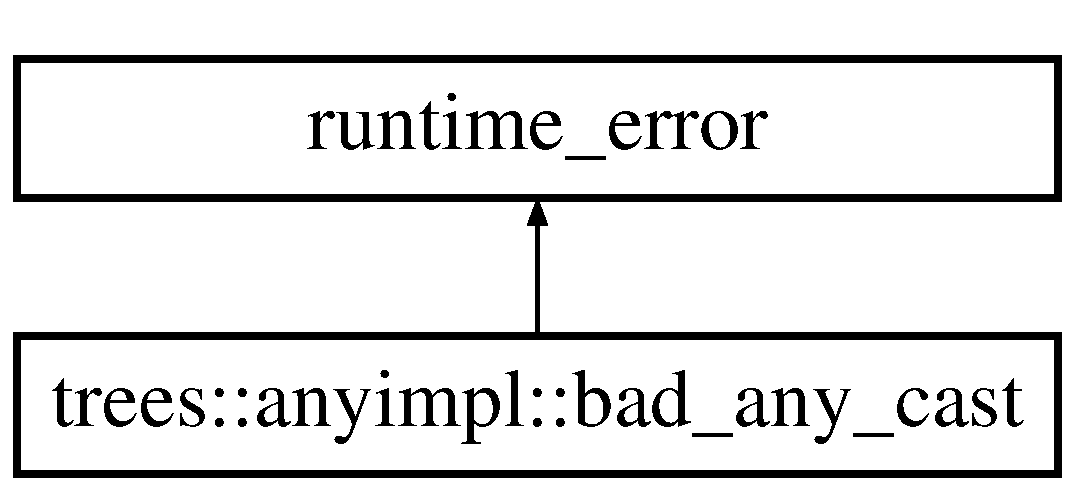
\includegraphics[height=2.000000cm]{structtrees_1_1anyimpl_1_1bad__any__cast}
\end{center}
\end{figure}


The documentation for this struct was generated from the following file\+:\begin{DoxyCompactItemize}
\item 
util/any.\+h\end{DoxyCompactItemize}

\hypertarget{structtrees_1_1anyimpl_1_1base__any__policy}{}\section{trees\+:\+:anyimpl\+:\+:base\+\_\+any\+\_\+policy Struct Reference}
\label{structtrees_1_1anyimpl_1_1base__any__policy}\index{trees\+::anyimpl\+::base\+\_\+any\+\_\+policy@{trees\+::anyimpl\+::base\+\_\+any\+\_\+policy}}
Inheritance diagram for trees\+:\+:anyimpl\+:\+:base\+\_\+any\+\_\+policy\+:\begin{figure}[H]
\begin{center}
\leavevmode
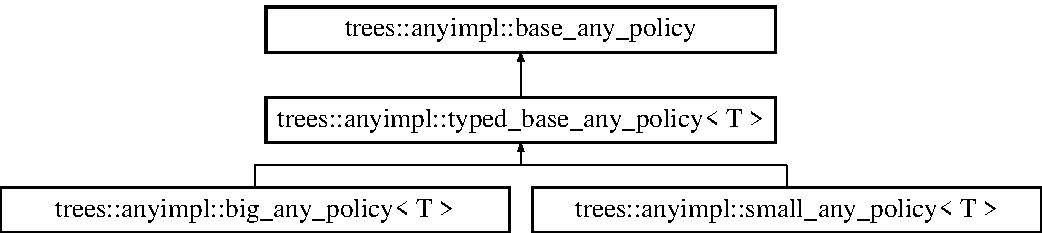
\includegraphics[height=3.000000cm]{structtrees_1_1anyimpl_1_1base__any__policy}
\end{center}
\end{figure}
\subsection*{Public Member Functions}
\begin{DoxyCompactItemize}
\item 
\mbox{\Hypertarget{structtrees_1_1anyimpl_1_1base__any__policy_a1903b2367ed09fa09e1e713098bf2e4f}\label{structtrees_1_1anyimpl_1_1base__any__policy_a1903b2367ed09fa09e1e713098bf2e4f}} 
virtual void {\bfseries static\+\_\+delete} (void $\ast$$\ast$x)=0
\item 
\mbox{\Hypertarget{structtrees_1_1anyimpl_1_1base__any__policy_ac8daab6d784a637d67bb7f11f71f95ae}\label{structtrees_1_1anyimpl_1_1base__any__policy_ac8daab6d784a637d67bb7f11f71f95ae}} 
virtual void {\bfseries copy\+\_\+from\+\_\+value} (void const $\ast$src, void $\ast$$\ast$dest)=0
\item 
\mbox{\Hypertarget{structtrees_1_1anyimpl_1_1base__any__policy_a82c84416680aa71ec9cf68d4c987f299}\label{structtrees_1_1anyimpl_1_1base__any__policy_a82c84416680aa71ec9cf68d4c987f299}} 
virtual void {\bfseries clone} (void $\ast$const $\ast$src, void $\ast$$\ast$dest)=0
\item 
\mbox{\Hypertarget{structtrees_1_1anyimpl_1_1base__any__policy_a4bca59609ae5fc7ebc9bbe20fc8d0686}\label{structtrees_1_1anyimpl_1_1base__any__policy_a4bca59609ae5fc7ebc9bbe20fc8d0686}} 
virtual void {\bfseries move} (void $\ast$const $\ast$src, void $\ast$$\ast$dest)=0
\item 
\mbox{\Hypertarget{structtrees_1_1anyimpl_1_1base__any__policy_adcd3a116177e228820e6b312b061c4f8}\label{structtrees_1_1anyimpl_1_1base__any__policy_adcd3a116177e228820e6b312b061c4f8}} 
virtual void $\ast$ {\bfseries get\+\_\+value} (void $\ast$$\ast$src)=0
\item 
\mbox{\Hypertarget{structtrees_1_1anyimpl_1_1base__any__policy_ae027b10d4a06a85a95c5ed974e0a210d}\label{structtrees_1_1anyimpl_1_1base__any__policy_ae027b10d4a06a85a95c5ed974e0a210d}} 
virtual const void $\ast$ {\bfseries get\+\_\+value} (void $\ast$const $\ast$src)=0
\item 
\mbox{\Hypertarget{structtrees_1_1anyimpl_1_1base__any__policy_a02f38616030b7fd8c16ee64496c9d851}\label{structtrees_1_1anyimpl_1_1base__any__policy_a02f38616030b7fd8c16ee64496c9d851}} 
virtual \+::size\+\_\+t {\bfseries get\+\_\+size} ()=0
\item 
\mbox{\Hypertarget{structtrees_1_1anyimpl_1_1base__any__policy_abc06c39bfd9c3c09d04a4f2abd30efa1}\label{structtrees_1_1anyimpl_1_1base__any__policy_abc06c39bfd9c3c09d04a4f2abd30efa1}} 
virtual const std\+::type\+\_\+info \& {\bfseries type} ()=0
\item 
\mbox{\Hypertarget{structtrees_1_1anyimpl_1_1base__any__policy_a993b0181f080c500084eb969e33ba7cc}\label{structtrees_1_1anyimpl_1_1base__any__policy_a993b0181f080c500084eb969e33ba7cc}} 
virtual void {\bfseries print} (std\+::ostream \&out, void $\ast$const $\ast$src)=0
\end{DoxyCompactItemize}


The documentation for this struct was generated from the following file\+:\begin{DoxyCompactItemize}
\item 
util/any.\+h\end{DoxyCompactItemize}

\hypertarget{structtrees_1_1anyimpl_1_1big__any__policy}{}\section{trees\+:\+:anyimpl\+:\+:big\+\_\+any\+\_\+policy$<$ T $>$ Struct Template Reference}
\label{structtrees_1_1anyimpl_1_1big__any__policy}\index{trees\+::anyimpl\+::big\+\_\+any\+\_\+policy$<$ T $>$@{trees\+::anyimpl\+::big\+\_\+any\+\_\+policy$<$ T $>$}}
Inheritance diagram for trees\+:\+:anyimpl\+:\+:big\+\_\+any\+\_\+policy$<$ T $>$\+:\begin{figure}[H]
\begin{center}
\leavevmode
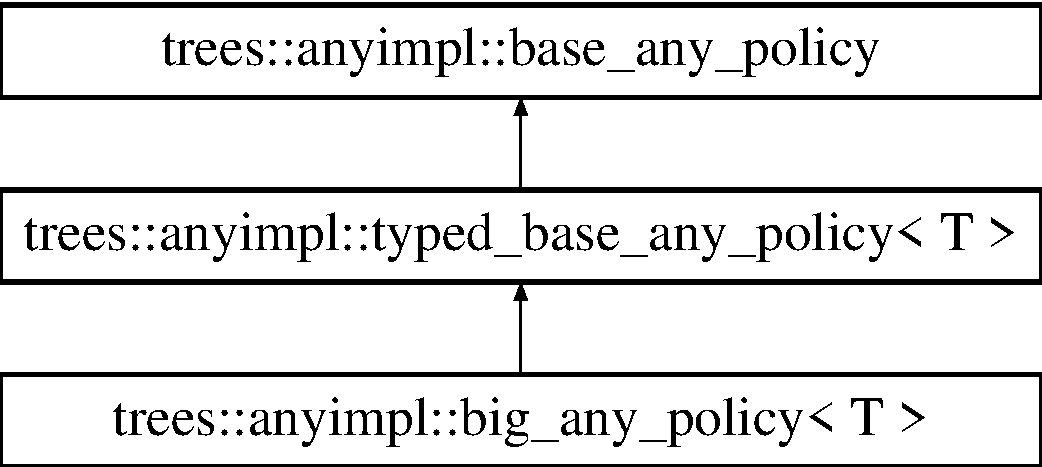
\includegraphics[height=3.000000cm]{structtrees_1_1anyimpl_1_1big__any__policy}
\end{center}
\end{figure}
\subsection*{Public Member Functions}
\begin{DoxyCompactItemize}
\item 
\mbox{\Hypertarget{structtrees_1_1anyimpl_1_1big__any__policy_a9a8ea0c5cd0437b145894c70f2b15579}\label{structtrees_1_1anyimpl_1_1big__any__policy_a9a8ea0c5cd0437b145894c70f2b15579}} 
virtual void {\bfseries static\+\_\+delete} (void $\ast$$\ast$x)
\item 
\mbox{\Hypertarget{structtrees_1_1anyimpl_1_1big__any__policy_aeb0656a2273d0705996467b8cf731ed9}\label{structtrees_1_1anyimpl_1_1big__any__policy_aeb0656a2273d0705996467b8cf731ed9}} 
virtual void {\bfseries copy\+\_\+from\+\_\+value} (void const $\ast$src, void $\ast$$\ast$dest)
\item 
\mbox{\Hypertarget{structtrees_1_1anyimpl_1_1big__any__policy_a2a79012e6153f04843bba9677f7593c1}\label{structtrees_1_1anyimpl_1_1big__any__policy_a2a79012e6153f04843bba9677f7593c1}} 
virtual void {\bfseries clone} (void $\ast$const $\ast$src, void $\ast$$\ast$dest)
\item 
\mbox{\Hypertarget{structtrees_1_1anyimpl_1_1big__any__policy_ad1e9d6e184cb858290a2ffd0bf6cf345}\label{structtrees_1_1anyimpl_1_1big__any__policy_ad1e9d6e184cb858290a2ffd0bf6cf345}} 
virtual void {\bfseries move} (void $\ast$const $\ast$src, void $\ast$$\ast$dest)
\item 
\mbox{\Hypertarget{structtrees_1_1anyimpl_1_1big__any__policy_a91205cd7307664b48ae668d90ff3cb27}\label{structtrees_1_1anyimpl_1_1big__any__policy_a91205cd7307664b48ae668d90ff3cb27}} 
virtual void $\ast$ {\bfseries get\+\_\+value} (void $\ast$$\ast$src)
\item 
\mbox{\Hypertarget{structtrees_1_1anyimpl_1_1big__any__policy_aede1f51b8cba7656baf5367d5f4b8fbb}\label{structtrees_1_1anyimpl_1_1big__any__policy_aede1f51b8cba7656baf5367d5f4b8fbb}} 
virtual const void $\ast$ {\bfseries get\+\_\+value} (void $\ast$const $\ast$src)
\item 
\mbox{\Hypertarget{structtrees_1_1anyimpl_1_1big__any__policy_a574865dc6e71801333cb58e21882cd3d}\label{structtrees_1_1anyimpl_1_1big__any__policy_a574865dc6e71801333cb58e21882cd3d}} 
virtual void {\bfseries print} (std\+::ostream \&out, void $\ast$const $\ast$src)
\end{DoxyCompactItemize}


The documentation for this struct was generated from the following file\+:\begin{DoxyCompactItemize}
\item 
util/any.\+h\end{DoxyCompactItemize}

\hypertarget{structtrees_1_1_branch_struct}{}\section{trees\+:\+:Branch\+Struct$<$ T, Distance\+Type $>$ Struct Template Reference}
\label{structtrees_1_1_branch_struct}\index{trees\+::\+Branch\+Struct$<$ T, Distance\+Type $>$@{trees\+::\+Branch\+Struct$<$ T, Distance\+Type $>$}}
\subsection*{Public Member Functions}
\begin{DoxyCompactItemize}
\item 
\mbox{\Hypertarget{structtrees_1_1_branch_struct_a7f2c8a75382a0b48aa8342ed65fb0b19}\label{structtrees_1_1_branch_struct_a7f2c8a75382a0b48aa8342ed65fb0b19}} 
{\bfseries Branch\+Struct} (const T \&a\+Node, Distance\+Type dist)
\item 
\mbox{\Hypertarget{structtrees_1_1_branch_struct_aaf0c81accb385dee2560d1157eac9a5e}\label{structtrees_1_1_branch_struct_aaf0c81accb385dee2560d1157eac9a5e}} 
{\bfseries Branch\+Struct} (const T \&a\+Node, Distance\+Type dist, Distance\+Type $\ast$dists\+\_\+)
\item 
\mbox{\Hypertarget{structtrees_1_1_branch_struct_a09ce496507ee30a910bcda1d4c65ab89}\label{structtrees_1_1_branch_struct_a09ce496507ee30a910bcda1d4c65ab89}} 
void {\bfseries clear} ()
\item 
\mbox{\Hypertarget{structtrees_1_1_branch_struct_a760336c1aab5e59227bfdbe0e6a56462}\label{structtrees_1_1_branch_struct_a760336c1aab5e59227bfdbe0e6a56462}} 
bool {\bfseries operator$<$} (const \hyperlink{structtrees_1_1_branch_struct}{Branch\+Struct}$<$ T, Distance\+Type $>$ \&rhs) const
\end{DoxyCompactItemize}
\subsection*{Public Attributes}
\begin{DoxyCompactItemize}
\item 
\mbox{\Hypertarget{structtrees_1_1_branch_struct_a1bd0cc2136455fb1da2c7cb00bb575ed}\label{structtrees_1_1_branch_struct_a1bd0cc2136455fb1da2c7cb00bb575ed}} 
T {\bfseries node}
\item 
\mbox{\Hypertarget{structtrees_1_1_branch_struct_a94935ab23accd67809ddf383357731dc}\label{structtrees_1_1_branch_struct_a94935ab23accd67809ddf383357731dc}} 
Distance\+Type {\bfseries mindist}
\item 
\mbox{\Hypertarget{structtrees_1_1_branch_struct_a07d1fdf824f99318047b219118ebb250}\label{structtrees_1_1_branch_struct_a07d1fdf824f99318047b219118ebb250}} 
Distance\+Type $\ast$ {\bfseries dists}
\end{DoxyCompactItemize}


The documentation for this struct was generated from the following file\+:\begin{DoxyCompactItemize}
\item 
utils/result\+\_\+set.\+h\end{DoxyCompactItemize}

\hypertarget{structtrees_1_1anyimpl_1_1choose__policy}{}\section{trees\+:\+:anyimpl\+:\+:choose\+\_\+policy$<$ T $>$ Struct Template Reference}
\label{structtrees_1_1anyimpl_1_1choose__policy}\index{trees\+::anyimpl\+::choose\+\_\+policy$<$ T $>$@{trees\+::anyimpl\+::choose\+\_\+policy$<$ T $>$}}
\subsection*{Public Types}
\begin{DoxyCompactItemize}
\item 
\mbox{\Hypertarget{structtrees_1_1anyimpl_1_1choose__policy_a0793f64590b26da57acc9f662cdfb2d0}\label{structtrees_1_1anyimpl_1_1choose__policy_a0793f64590b26da57acc9f662cdfb2d0}} 
typedef \hyperlink{structtrees_1_1anyimpl_1_1big__any__policy}{big\+\_\+any\+\_\+policy}$<$ T $>$ {\bfseries type}
\end{DoxyCompactItemize}


The documentation for this struct was generated from the following file\+:\begin{DoxyCompactItemize}
\item 
util/any.\+h\end{DoxyCompactItemize}

\hypertarget{structtrees_1_1anyimpl_1_1choose__policy_3_01any_01_4}{}\section{trees\+:\+:anyimpl\+:\+:choose\+\_\+policy$<$ any $>$ Struct Template Reference}
\label{structtrees_1_1anyimpl_1_1choose__policy_3_01any_01_4}\index{trees\+::anyimpl\+::choose\+\_\+policy$<$ any $>$@{trees\+::anyimpl\+::choose\+\_\+policy$<$ any $>$}}


{\ttfamily \#include $<$any.\+h$>$}

\subsection*{Public Types}
\begin{DoxyCompactItemize}
\item 
\mbox{\Hypertarget{structtrees_1_1anyimpl_1_1choose__policy_3_01any_01_4_a2d661f31e7a16ed78096e4a2bcdf365d}\label{structtrees_1_1anyimpl_1_1choose__policy_3_01any_01_4_a2d661f31e7a16ed78096e4a2bcdf365d}} 
typedef void {\bfseries type}
\end{DoxyCompactItemize}


\subsection{Detailed Description}
\subsubsection*{template$<$$>$\newline
struct trees\+::anyimpl\+::choose\+\_\+policy$<$ any $>$}

Choosing the policy for an any type is illegal, but should never happen. This is designed to throw a compiler error. 

The documentation for this struct was generated from the following file\+:\begin{DoxyCompactItemize}
\item 
util/any.\+h\end{DoxyCompactItemize}

\hypertarget{structtrees_1_1anyimpl_1_1choose__policy_3_01_t_01_5_01_4}{}\section{trees\+:\+:anyimpl\+:\+:choose\+\_\+policy$<$ T $\ast$ $>$ Struct Template Reference}
\label{structtrees_1_1anyimpl_1_1choose__policy_3_01_t_01_5_01_4}\index{trees\+::anyimpl\+::choose\+\_\+policy$<$ T $\ast$ $>$@{trees\+::anyimpl\+::choose\+\_\+policy$<$ T $\ast$ $>$}}
\subsection*{Public Types}
\begin{DoxyCompactItemize}
\item 
\mbox{\Hypertarget{structtrees_1_1anyimpl_1_1choose__policy_3_01_t_01_5_01_4_a209d5e160fad2f278728b0005c643fff}\label{structtrees_1_1anyimpl_1_1choose__policy_3_01_t_01_5_01_4_a209d5e160fad2f278728b0005c643fff}} 
typedef \hyperlink{structtrees_1_1anyimpl_1_1small__any__policy}{small\+\_\+any\+\_\+policy}$<$ T $\ast$ $>$ {\bfseries type}
\end{DoxyCompactItemize}


The documentation for this struct was generated from the following file\+:\begin{DoxyCompactItemize}
\item 
util/any.\+h\end{DoxyCompactItemize}

\hypertarget{classtrees_1_1_count_radius_result_set}{}\section{trees\+:\+:Count\+Radius\+Result\+Set$<$ Distance\+Type $>$ Class Template Reference}
\label{classtrees_1_1_count_radius_result_set}\index{trees\+::\+Count\+Radius\+Result\+Set$<$ Distance\+Type $>$@{trees\+::\+Count\+Radius\+Result\+Set$<$ Distance\+Type $>$}}


{\ttfamily \#include $<$result\+\_\+set.\+h$>$}

Inheritance diagram for trees\+:\+:Count\+Radius\+Result\+Set$<$ Distance\+Type $>$\+:\begin{figure}[H]
\begin{center}
\leavevmode
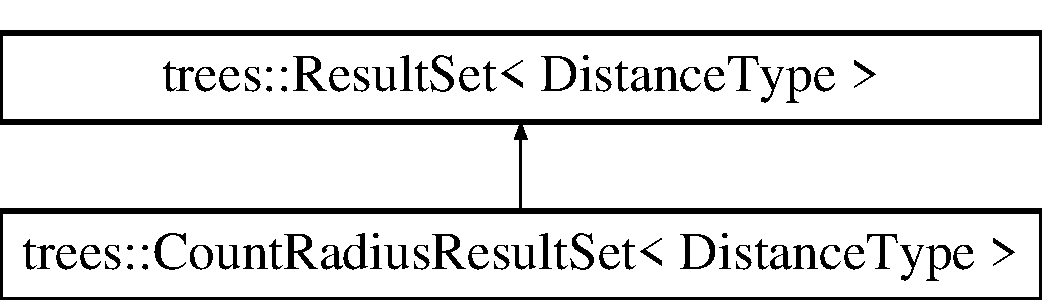
\includegraphics[height=2.000000cm]{classtrees_1_1_count_radius_result_set}
\end{center}
\end{figure}
\subsection*{Public Member Functions}
\begin{DoxyCompactItemize}
\item 
\mbox{\Hypertarget{classtrees_1_1_count_radius_result_set_ac43b2810f33cfea632f514bbce78b20f}\label{classtrees_1_1_count_radius_result_set_ac43b2810f33cfea632f514bbce78b20f}} 
{\bfseries Count\+Radius\+Result\+Set} (Distance\+Type radius\+\_\+)
\item 
\mbox{\Hypertarget{classtrees_1_1_count_radius_result_set_a7f5c3d6831610ee002bc2372fbf28eef}\label{classtrees_1_1_count_radius_result_set_a7f5c3d6831610ee002bc2372fbf28eef}} 
void {\bfseries clear} ()
\item 
\mbox{\Hypertarget{classtrees_1_1_count_radius_result_set_a292fb4fa1d8690f33fcf988d59c85922}\label{classtrees_1_1_count_radius_result_set_a292fb4fa1d8690f33fcf988d59c85922}} 
size\+\_\+t {\bfseries size} () const
\item 
\mbox{\Hypertarget{classtrees_1_1_count_radius_result_set_ad9f498bee21c16052b36fd852c338143}\label{classtrees_1_1_count_radius_result_set_ad9f498bee21c16052b36fd852c338143}} 
bool {\bfseries full} () const
\item 
\mbox{\Hypertarget{classtrees_1_1_count_radius_result_set_ad91ad04231f5256444c2b0684e519252}\label{classtrees_1_1_count_radius_result_set_ad91ad04231f5256444c2b0684e519252}} 
void {\bfseries add\+Point} (Distance\+Type dist, size\+\_\+t index)
\item 
\mbox{\Hypertarget{classtrees_1_1_count_radius_result_set_afe11310933b2e5b27b5b5b2fc4cf25ac}\label{classtrees_1_1_count_radius_result_set_afe11310933b2e5b27b5b5b2fc4cf25ac}} 
Distance\+Type {\bfseries worst\+Dist} () const
\end{DoxyCompactItemize}
\subsection*{Additional Inherited Members}


\subsection{Detailed Description}
\subsubsection*{template$<$typename Distance\+Type$>$\newline
class trees\+::\+Count\+Radius\+Result\+Set$<$ Distance\+Type $>$}

This is a result set that only counts the neighbors within a radius. 

The documentation for this class was generated from the following file\+:\begin{DoxyCompactItemize}
\item 
util/result\+\_\+set.\+h\end{DoxyCompactItemize}

\hypertarget{structtrees_1_1_distance_index}{}\section{trees\+:\+:Distance\+Index$<$ Distance\+Type $>$ Struct Template Reference}
\label{structtrees_1_1_distance_index}\index{trees\+::\+Distance\+Index$<$ Distance\+Type $>$@{trees\+::\+Distance\+Index$<$ Distance\+Type $>$}}
\subsection*{Public Member Functions}
\begin{DoxyCompactItemize}
\item 
\mbox{\Hypertarget{structtrees_1_1_distance_index_a90ce5ece57dc6f6807a3af01f8185ab3}\label{structtrees_1_1_distance_index_a90ce5ece57dc6f6807a3af01f8185ab3}} 
{\bfseries Distance\+Index} (Distance\+Type dist, size\+\_\+t index)
\item 
\mbox{\Hypertarget{structtrees_1_1_distance_index_a244d8c16ca20d24b3d674cc597c0593a}\label{structtrees_1_1_distance_index_a244d8c16ca20d24b3d674cc597c0593a}} 
bool {\bfseries operator$<$} (const \hyperlink{structtrees_1_1_distance_index}{Distance\+Index} \&dist\+\_\+index) const
\end{DoxyCompactItemize}
\subsection*{Public Attributes}
\begin{DoxyCompactItemize}
\item 
\mbox{\Hypertarget{structtrees_1_1_distance_index_a21357a72377919a1f39016632e07eefc}\label{structtrees_1_1_distance_index_a21357a72377919a1f39016632e07eefc}} 
Distance\+Type {\bfseries dist\+\_\+}
\item 
\mbox{\Hypertarget{structtrees_1_1_distance_index_a8c9025202c2717d9271507e4ca4d7611}\label{structtrees_1_1_distance_index_a8c9025202c2717d9271507e4ca4d7611}} 
size\+\_\+t {\bfseries index\+\_\+}
\end{DoxyCompactItemize}


The documentation for this struct was generated from the following file\+:\begin{DoxyCompactItemize}
\item 
utils/result\+\_\+set.\+h\end{DoxyCompactItemize}

\hypertarget{structtrees_1_1_unique_result_set_1_1_dist_index}{}\section{trees\+:\+:Unique\+Result\+Set$<$ Distance\+Type $>$\+:\+:Dist\+Index Struct Reference}
\label{structtrees_1_1_unique_result_set_1_1_dist_index}\index{trees\+::\+Unique\+Result\+Set$<$ Distance\+Type $>$\+::\+Dist\+Index@{trees\+::\+Unique\+Result\+Set$<$ Distance\+Type $>$\+::\+Dist\+Index}}
\subsection*{Public Member Functions}
\begin{DoxyCompactItemize}
\item 
\mbox{\Hypertarget{structtrees_1_1_unique_result_set_1_1_dist_index_aac8345219321567db4a9ccd0da7ed827}\label{structtrees_1_1_unique_result_set_1_1_dist_index_aac8345219321567db4a9ccd0da7ed827}} 
{\bfseries Dist\+Index} (Distance\+Type dist, unsigned int index)
\item 
\mbox{\Hypertarget{structtrees_1_1_unique_result_set_1_1_dist_index_abf0c04fdea75664003b96a0f8735c017}\label{structtrees_1_1_unique_result_set_1_1_dist_index_abf0c04fdea75664003b96a0f8735c017}} 
bool {\bfseries operator$<$} (const \hyperlink{structtrees_1_1_unique_result_set_1_1_dist_index}{Dist\+Index} dist\+\_\+index) const
\end{DoxyCompactItemize}
\subsection*{Public Attributes}
\begin{DoxyCompactItemize}
\item 
\mbox{\Hypertarget{structtrees_1_1_unique_result_set_1_1_dist_index_aa382acdc4be772e9788f1d77a1cfa247}\label{structtrees_1_1_unique_result_set_1_1_dist_index_aa382acdc4be772e9788f1d77a1cfa247}} 
Distance\+Type {\bfseries dist\+\_\+}
\item 
\mbox{\Hypertarget{structtrees_1_1_unique_result_set_1_1_dist_index_a2ad613379c6478910c675a86e9aac5cd}\label{structtrees_1_1_unique_result_set_1_1_dist_index_a2ad613379c6478910c675a86e9aac5cd}} 
unsigned int {\bfseries index\+\_\+}
\end{DoxyCompactItemize}


The documentation for this struct was generated from the following file\+:\begin{DoxyCompactItemize}
\item 
util/result\+\_\+set.\+h\end{DoxyCompactItemize}

\hypertarget{structtrees_1_1anyimpl_1_1empty__any}{}\section{trees\+:\+:anyimpl\+:\+:empty\+\_\+any Struct Reference}
\label{structtrees_1_1anyimpl_1_1empty__any}\index{trees\+::anyimpl\+::empty\+\_\+any@{trees\+::anyimpl\+::empty\+\_\+any}}


The documentation for this struct was generated from the following file\+:\begin{DoxyCompactItemize}
\item 
util/any.\+h\end{DoxyCompactItemize}

\hypertarget{classtrees_1_1_index}{}\section{trees\+:\+:Index$<$ Element\+Type $>$ Class Template Reference}
\label{classtrees_1_1_index}\index{trees\+::\+Index$<$ Element\+Type $>$@{trees\+::\+Index$<$ Element\+Type $>$}}
\subsection*{Public Member Functions}
\begin{DoxyCompactItemize}
\item 
\hyperlink{classtrees_1_1_index_a8ac9a102556cdf044f3384305b713d6d}{Index} (const \hyperlink{classtrees_1_1_matrix}{Matrix}$<$ Element\+Type $>$ \&dataset\+\_\+, const Index\+Params \&params\+\_\+)
\item 
void \hyperlink{classtrees_1_1_index_a3bbc8a66a33309b8f2f320d726ecabc9}{free\+Index} ()
\item 
void \hyperlink{classtrees_1_1_index_a56f07dc136d2fff0fc81633cd9bb78fb}{get\+Dataset} (\hyperlink{classtrees_1_1_matrix}{Matrix}$<$ Element\+Type $>$ \&dataset\+\_\+)
\item 
void \hyperlink{classtrees_1_1_index_a893641c30781d8d75b4e22135f0cbd3e}{build\+Index} ()
\item 
void \hyperlink{classtrees_1_1_index_af82fc39c391107cc9d35a3b6c14fcdc6}{rebuild} (const \hyperlink{classtrees_1_1_matrix}{Matrix}$<$ Element\+Type $>$ \&dataset\+\_\+)
\item 
bool \hyperlink{classtrees_1_1_index_ad506d4fd5a9c35a1e86d2241b7f8c370}{remove} (size\+\_\+t index\+\_\+)
\item 
void \hyperlink{classtrees_1_1_index_a716c861946ed217622a9cfc60d25196f}{knn\+Search} (const \hyperlink{classtrees_1_1_matrix}{Matrix}$<$ Element\+Type $>$ \&queries\+\_\+, \hyperlink{classtrees_1_1_matrix}{Matrix}$<$ size\+\_\+t $>$ \&indices\+\_\+, \hyperlink{classtrees_1_1_matrix}{Matrix}$<$ Element\+Type $>$ \&dists\+\_\+, size\+\_\+t knn\+\_\+, const \hyperlink{structtrees_1_1_tree_params}{Tree\+Params} \&params\+\_\+)
\item 
void \hyperlink{classtrees_1_1_index_a50aa3029ca0fc9eb3d2bb4c5d0f8e71a}{knn\+Search} (const \hyperlink{classtrees_1_1_matrix}{Matrix}$<$ Element\+Type $>$ \&queries\+\_\+, \hyperlink{classtrees_1_1_matrix}{Matrix}$<$ int $>$ \&indices\+\_\+, \hyperlink{classtrees_1_1_matrix}{Matrix}$<$ Element\+Type $>$ \&dists\+\_\+, size\+\_\+t knn\+\_\+, const \hyperlink{structtrees_1_1_tree_params}{Tree\+Params} \&params\+\_\+)
\item 
void \hyperlink{classtrees_1_1_index_afc97b459d0dc05fcce4dea3f75b248aa}{radius\+Search} (const \hyperlink{classtrees_1_1_matrix}{Matrix}$<$ Element\+Type $>$ \&queries\+\_\+, std\+::vector$<$ std\+::vector$<$ size\+\_\+t $>$$>$ \&indices\+\_\+, std\+::vector$<$ std\+::vector$<$ Element\+Type $>$$>$ \&dists\+\_\+, float radius\+\_\+, const \hyperlink{structtrees_1_1_tree_params}{Tree\+Params} \&params\+\_\+)
\item 
void \hyperlink{classtrees_1_1_index_aefb21018541d6a06a382f579f78819e6}{radius\+Search} (const \hyperlink{classtrees_1_1_matrix}{Matrix}$<$ Element\+Type $>$ \&queries\+\_\+, std\+::vector$<$ std\+::vector$<$ int $>$$>$ \&indices\+\_\+, std\+::vector$<$ std\+::vector$<$ Element\+Type $>$$>$ \&dists\+\_\+, float radius\+\_\+, const \hyperlink{structtrees_1_1_tree_params}{Tree\+Params} \&params\+\_\+)
\end{DoxyCompactItemize}


\subsection{Constructor \& Destructor Documentation}
\mbox{\Hypertarget{classtrees_1_1_index_a8ac9a102556cdf044f3384305b713d6d}\label{classtrees_1_1_index_a8ac9a102556cdf044f3384305b713d6d}} 
\index{trees\+::\+Index@{trees\+::\+Index}!Index@{Index}}
\index{Index@{Index}!trees\+::\+Index@{trees\+::\+Index}}
\subsubsection{\texorpdfstring{Index()}{Index()}}
{\footnotesize\ttfamily template$<$typename Element\+Type $>$ \\
\hyperlink{classtrees_1_1_index}{trees\+::\+Index}$<$ Element\+Type $>$\+::\hyperlink{classtrees_1_1_index}{Index} (\begin{DoxyParamCaption}\item[{const \hyperlink{classtrees_1_1_matrix}{Matrix}$<$ Element\+Type $>$ \&}]{dataset\+\_\+,  }\item[{const Index\+Params \&}]{params\+\_\+ }\end{DoxyParamCaption})\hspace{0.3cm}{\ttfamily [inline]}}

Constructor


\begin{DoxyParams}[1]{Parameters}
\mbox{\tt in}  & {\em dataset\+\_\+} & Pointcloud \\
\hline
\mbox{\tt in}  & {\em params\+\_\+} & Input parameters \\
\hline
\end{DoxyParams}


\subsection{Member Function Documentation}
\mbox{\Hypertarget{classtrees_1_1_index_a893641c30781d8d75b4e22135f0cbd3e}\label{classtrees_1_1_index_a893641c30781d8d75b4e22135f0cbd3e}} 
\index{trees\+::\+Index@{trees\+::\+Index}!build\+Index@{build\+Index}}
\index{build\+Index@{build\+Index}!trees\+::\+Index@{trees\+::\+Index}}
\subsubsection{\texorpdfstring{build\+Index()}{buildIndex()}}
{\footnotesize\ttfamily template$<$typename Element\+Type $>$ \\
void \hyperlink{classtrees_1_1_index}{trees\+::\+Index}$<$ Element\+Type $>$\+::build\+Index (\begin{DoxyParamCaption}{ }\end{DoxyParamCaption})\hspace{0.3cm}{\ttfamily [inline]}}

Build the tree \mbox{\Hypertarget{classtrees_1_1_index_a3bbc8a66a33309b8f2f320d726ecabc9}\label{classtrees_1_1_index_a3bbc8a66a33309b8f2f320d726ecabc9}} 
\index{trees\+::\+Index@{trees\+::\+Index}!free\+Index@{free\+Index}}
\index{free\+Index@{free\+Index}!trees\+::\+Index@{trees\+::\+Index}}
\subsubsection{\texorpdfstring{free\+Index()}{freeIndex()}}
{\footnotesize\ttfamily template$<$typename Element\+Type $>$ \\
void \hyperlink{classtrees_1_1_index}{trees\+::\+Index}$<$ Element\+Type $>$\+::free\+Index (\begin{DoxyParamCaption}{ }\end{DoxyParamCaption})\hspace{0.3cm}{\ttfamily [inline]}}

Frees allocated memory \mbox{\Hypertarget{classtrees_1_1_index_a56f07dc136d2fff0fc81633cd9bb78fb}\label{classtrees_1_1_index_a56f07dc136d2fff0fc81633cd9bb78fb}} 
\index{trees\+::\+Index@{trees\+::\+Index}!get\+Dataset@{get\+Dataset}}
\index{get\+Dataset@{get\+Dataset}!trees\+::\+Index@{trees\+::\+Index}}
\subsubsection{\texorpdfstring{get\+Dataset()}{getDataset()}}
{\footnotesize\ttfamily template$<$typename Element\+Type $>$ \\
void \hyperlink{classtrees_1_1_index}{trees\+::\+Index}$<$ Element\+Type $>$\+::get\+Dataset (\begin{DoxyParamCaption}\item[{\hyperlink{classtrees_1_1_matrix}{Matrix}$<$ Element\+Type $>$ \&}]{dataset\+\_\+ }\end{DoxyParamCaption})\hspace{0.3cm}{\ttfamily [inline]}}

Get the dataset \mbox{\Hypertarget{classtrees_1_1_index_a716c861946ed217622a9cfc60d25196f}\label{classtrees_1_1_index_a716c861946ed217622a9cfc60d25196f}} 
\index{trees\+::\+Index@{trees\+::\+Index}!knn\+Search@{knn\+Search}}
\index{knn\+Search@{knn\+Search}!trees\+::\+Index@{trees\+::\+Index}}
\subsubsection{\texorpdfstring{knn\+Search()}{knnSearch()}\hspace{0.1cm}{\footnotesize\ttfamily [1/2]}}
{\footnotesize\ttfamily template$<$typename Element\+Type $>$ \\
void \hyperlink{classtrees_1_1_index}{trees\+::\+Index}$<$ Element\+Type $>$\+::knn\+Search (\begin{DoxyParamCaption}\item[{const \hyperlink{classtrees_1_1_matrix}{Matrix}$<$ Element\+Type $>$ \&}]{queries\+\_\+,  }\item[{\hyperlink{classtrees_1_1_matrix}{Matrix}$<$ size\+\_\+t $>$ \&}]{indices\+\_\+,  }\item[{\hyperlink{classtrees_1_1_matrix}{Matrix}$<$ Element\+Type $>$ \&}]{dists\+\_\+,  }\item[{size\+\_\+t}]{knn\+\_\+,  }\item[{const \hyperlink{structtrees_1_1_tree_params}{Tree\+Params} \&}]{params\+\_\+ }\end{DoxyParamCaption})\hspace{0.3cm}{\ttfamily [inline]}}

Perform k-\/nearest neighbor search


\begin{DoxyParams}[1]{Parameters}
\mbox{\tt in}  & {\em queries\+\_\+} & The query points for which to find the nearest neighbors \\
\hline
\mbox{\tt in,out}  & {\em indices\+\_\+} & The indices of the nearest neighbors found \\
\hline
\mbox{\tt in,out}  & {\em dists\+\_\+} & Distances to the nearest neighbors found \\
\hline
\mbox{\tt in}  & {\em knn\+\_\+} & Number of nearest neighbors to return \\
\hline
\mbox{\tt in}  & {\em params\+\_\+} & Search parameters \\
\hline
\end{DoxyParams}
\mbox{\Hypertarget{classtrees_1_1_index_a50aa3029ca0fc9eb3d2bb4c5d0f8e71a}\label{classtrees_1_1_index_a50aa3029ca0fc9eb3d2bb4c5d0f8e71a}} 
\index{trees\+::\+Index@{trees\+::\+Index}!knn\+Search@{knn\+Search}}
\index{knn\+Search@{knn\+Search}!trees\+::\+Index@{trees\+::\+Index}}
\subsubsection{\texorpdfstring{knn\+Search()}{knnSearch()}\hspace{0.1cm}{\footnotesize\ttfamily [2/2]}}
{\footnotesize\ttfamily template$<$typename Element\+Type $>$ \\
void \hyperlink{classtrees_1_1_index}{trees\+::\+Index}$<$ Element\+Type $>$\+::knn\+Search (\begin{DoxyParamCaption}\item[{const \hyperlink{classtrees_1_1_matrix}{Matrix}$<$ Element\+Type $>$ \&}]{queries\+\_\+,  }\item[{\hyperlink{classtrees_1_1_matrix}{Matrix}$<$ int $>$ \&}]{indices\+\_\+,  }\item[{\hyperlink{classtrees_1_1_matrix}{Matrix}$<$ Element\+Type $>$ \&}]{dists\+\_\+,  }\item[{size\+\_\+t}]{knn\+\_\+,  }\item[{const \hyperlink{structtrees_1_1_tree_params}{Tree\+Params} \&}]{params\+\_\+ }\end{DoxyParamCaption})\hspace{0.3cm}{\ttfamily [inline]}}

Perform k-\/nearest neighbor search


\begin{DoxyParams}[1]{Parameters}
\mbox{\tt in}  & {\em queries\+\_\+} & The query points for which to find the nearest neighbors \\
\hline
\mbox{\tt in,out}  & {\em indices\+\_\+} & The indices of the nearest neighbors found \\
\hline
\mbox{\tt in,out}  & {\em dists\+\_\+} & Distances to the nearest neighbors found \\
\hline
\mbox{\tt in}  & {\em knn\+\_\+} & Number of nearest neighbors to return \\
\hline
\mbox{\tt in}  & {\em params\+\_\+} & Search parameters \\
\hline
\end{DoxyParams}
\mbox{\Hypertarget{classtrees_1_1_index_afc97b459d0dc05fcce4dea3f75b248aa}\label{classtrees_1_1_index_afc97b459d0dc05fcce4dea3f75b248aa}} 
\index{trees\+::\+Index@{trees\+::\+Index}!radius\+Search@{radius\+Search}}
\index{radius\+Search@{radius\+Search}!trees\+::\+Index@{trees\+::\+Index}}
\subsubsection{\texorpdfstring{radius\+Search()}{radiusSearch()}\hspace{0.1cm}{\footnotesize\ttfamily [1/2]}}
{\footnotesize\ttfamily template$<$typename Element\+Type $>$ \\
void \hyperlink{classtrees_1_1_index}{trees\+::\+Index}$<$ Element\+Type $>$\+::radius\+Search (\begin{DoxyParamCaption}\item[{const \hyperlink{classtrees_1_1_matrix}{Matrix}$<$ Element\+Type $>$ \&}]{queries\+\_\+,  }\item[{std\+::vector$<$ std\+::vector$<$ size\+\_\+t $>$$>$ \&}]{indices\+\_\+,  }\item[{std\+::vector$<$ std\+::vector$<$ Element\+Type $>$$>$ \&}]{dists\+\_\+,  }\item[{float}]{radius\+\_\+,  }\item[{const \hyperlink{structtrees_1_1_tree_params}{Tree\+Params} \&}]{params\+\_\+ }\end{DoxyParamCaption})\hspace{0.3cm}{\ttfamily [inline]}}

Perform radius search


\begin{DoxyParams}[1]{Parameters}
\mbox{\tt in}  & {\em queries\+\_\+} & The query points for which to find the nearest neighbors \\
\hline
\mbox{\tt in,out}  & {\em indices\+\_\+} & The indices of the nearest neighbors found \\
\hline
\mbox{\tt in,out}  & {\em dists\+\_\+} & Distances to the nearest neighbors found \\
\hline
\mbox{\tt in}  & {\em radius\+\_\+} & The radius used for search \\
\hline
\mbox{\tt in}  & {\em params\+\_\+} & Search parameters \\
\hline
\end{DoxyParams}
\mbox{\Hypertarget{classtrees_1_1_index_aefb21018541d6a06a382f579f78819e6}\label{classtrees_1_1_index_aefb21018541d6a06a382f579f78819e6}} 
\index{trees\+::\+Index@{trees\+::\+Index}!radius\+Search@{radius\+Search}}
\index{radius\+Search@{radius\+Search}!trees\+::\+Index@{trees\+::\+Index}}
\subsubsection{\texorpdfstring{radius\+Search()}{radiusSearch()}\hspace{0.1cm}{\footnotesize\ttfamily [2/2]}}
{\footnotesize\ttfamily template$<$typename Element\+Type $>$ \\
void \hyperlink{classtrees_1_1_index}{trees\+::\+Index}$<$ Element\+Type $>$\+::radius\+Search (\begin{DoxyParamCaption}\item[{const \hyperlink{classtrees_1_1_matrix}{Matrix}$<$ Element\+Type $>$ \&}]{queries\+\_\+,  }\item[{std\+::vector$<$ std\+::vector$<$ int $>$$>$ \&}]{indices\+\_\+,  }\item[{std\+::vector$<$ std\+::vector$<$ Element\+Type $>$$>$ \&}]{dists\+\_\+,  }\item[{float}]{radius\+\_\+,  }\item[{const \hyperlink{structtrees_1_1_tree_params}{Tree\+Params} \&}]{params\+\_\+ }\end{DoxyParamCaption})\hspace{0.3cm}{\ttfamily [inline]}}

Perform radius search


\begin{DoxyParams}[1]{Parameters}
\mbox{\tt in}  & {\em queries\+\_\+} & The query points for which to find the nearest neighbors \\
\hline
\mbox{\tt in,out}  & {\em indices\+\_\+} & The indices of the nearest neighbors found \\
\hline
\mbox{\tt in,out}  & {\em dists\+\_\+} & Distances to the nearest neighbors found \\
\hline
\mbox{\tt in}  & {\em radius\+\_\+} & The radius used for search \\
\hline
\mbox{\tt in}  & {\em params\+\_\+} & Search parameters \\
\hline
\end{DoxyParams}
\mbox{\Hypertarget{classtrees_1_1_index_af82fc39c391107cc9d35a3b6c14fcdc6}\label{classtrees_1_1_index_af82fc39c391107cc9d35a3b6c14fcdc6}} 
\index{trees\+::\+Index@{trees\+::\+Index}!rebuild@{rebuild}}
\index{rebuild@{rebuild}!trees\+::\+Index@{trees\+::\+Index}}
\subsubsection{\texorpdfstring{rebuild()}{rebuild()}}
{\footnotesize\ttfamily template$<$typename Element\+Type $>$ \\
void \hyperlink{classtrees_1_1_index}{trees\+::\+Index}$<$ Element\+Type $>$\+::rebuild (\begin{DoxyParamCaption}\item[{const \hyperlink{classtrees_1_1_matrix}{Matrix}$<$ Element\+Type $>$ \&}]{dataset\+\_\+ }\end{DoxyParamCaption})\hspace{0.3cm}{\ttfamily [inline]}}

Rebuilds the index


\begin{DoxyParams}[1]{Parameters}
\mbox{\tt in}  & {\em dataset\+\_\+} & Pointcloud \\
\hline
\end{DoxyParams}
\mbox{\Hypertarget{classtrees_1_1_index_ad506d4fd5a9c35a1e86d2241b7f8c370}\label{classtrees_1_1_index_ad506d4fd5a9c35a1e86d2241b7f8c370}} 
\index{trees\+::\+Index@{trees\+::\+Index}!remove@{remove}}
\index{remove@{remove}!trees\+::\+Index@{trees\+::\+Index}}
\subsubsection{\texorpdfstring{remove()}{remove()}}
{\footnotesize\ttfamily template$<$typename Element\+Type $>$ \\
bool \hyperlink{classtrees_1_1_index}{trees\+::\+Index}$<$ Element\+Type $>$\+::remove (\begin{DoxyParamCaption}\item[{size\+\_\+t}]{index\+\_\+ }\end{DoxyParamCaption})\hspace{0.3cm}{\ttfamily [inline]}}

Removes point from kdtree


\begin{DoxyParams}[1]{Parameters}
\mbox{\tt in}  & {\em index\+\_\+} & \hyperlink{classtrees_1_1_index}{Index} of the point in the pointcloud \\
\hline
\end{DoxyParams}


The documentation for this class was generated from the following file\+:\begin{DoxyCompactItemize}
\item 
trees.\+hpp\end{DoxyCompactItemize}

\hypertarget{structtrees_1_1_k_d_tree_index_1_1_interval}{}\section{trees\+:\+:K\+D\+Tree\+Index$<$ Element\+Type $>$\+:\+:Interval Struct Reference}
\label{structtrees_1_1_k_d_tree_index_1_1_interval}\index{trees\+::\+K\+D\+Tree\+Index$<$ Element\+Type $>$\+::\+Interval@{trees\+::\+K\+D\+Tree\+Index$<$ Element\+Type $>$\+::\+Interval}}


{\ttfamily \#include $<$kdtree\+\_\+index.\+h$>$}

\subsection*{Public Attributes}
\begin{DoxyCompactItemize}
\item 
\mbox{\Hypertarget{structtrees_1_1_k_d_tree_index_1_1_interval_af0a3a4d4916319eb8b487aaee6ce3241}\label{structtrees_1_1_k_d_tree_index_1_1_interval_af0a3a4d4916319eb8b487aaee6ce3241}} 
Element\+Type {\bfseries low}
\item 
\mbox{\Hypertarget{structtrees_1_1_k_d_tree_index_1_1_interval_a1a77acac4f1ee40f913c2b64399b1d19}\label{structtrees_1_1_k_d_tree_index_1_1_interval_a1a77acac4f1ee40f913c2b64399b1d19}} 
Element\+Type {\bfseries high}
\end{DoxyCompactItemize}


\subsection{Detailed Description}
\subsubsection*{template$<$typename Element\+Type$>$\newline
struct trees\+::\+K\+D\+Tree\+Index$<$ Element\+Type $>$\+::\+Interval}

Structures for the bounding box 

The documentation for this struct was generated from the following file\+:\begin{DoxyCompactItemize}
\item 
algorithms/kdtree\+\_\+index.\+h\end{DoxyCompactItemize}

\hypertarget{classtrees_1_1_k_d_tree_index}{}\section{trees\+:\+:K\+D\+Tree\+Index$<$ Element\+Type $>$ Class Template Reference}
\label{classtrees_1_1_k_d_tree_index}\index{trees\+::\+K\+D\+Tree\+Index$<$ Element\+Type $>$@{trees\+::\+K\+D\+Tree\+Index$<$ Element\+Type $>$}}
Inheritance diagram for trees\+:\+:K\+D\+Tree\+Index$<$ Element\+Type $>$\+:\begin{figure}[H]
\begin{center}
\leavevmode
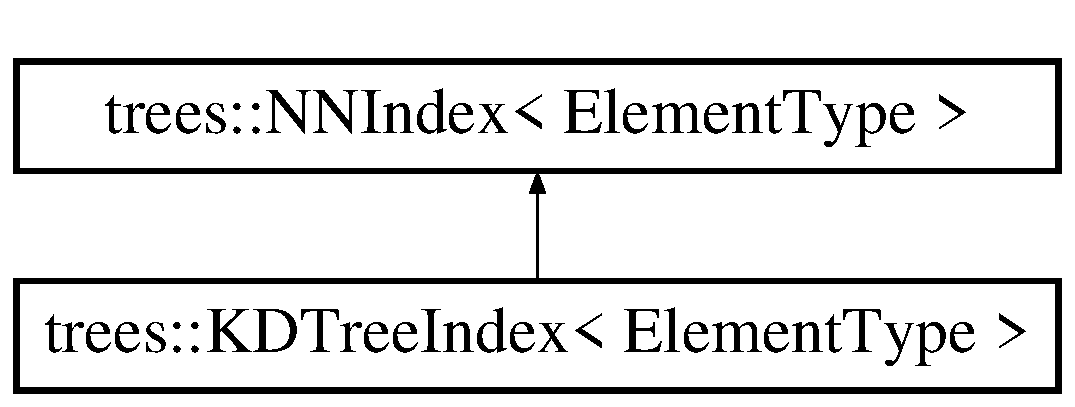
\includegraphics[height=2.000000cm]{classtrees_1_1_k_d_tree_index}
\end{center}
\end{figure}
\subsection*{Classes}
\begin{DoxyCompactItemize}
\item 
struct \hyperlink{structtrees_1_1_k_d_tree_index_1_1_interval}{Interval}
\item 
struct \hyperlink{structtrees_1_1_k_d_tree_index_1_1_node}{Node}
\end{DoxyCompactItemize}
\subsection*{Public Types}
\begin{DoxyCompactItemize}
\item 
\mbox{\Hypertarget{classtrees_1_1_k_d_tree_index_a18fc026725b0201b5086e03dd1904035}\label{classtrees_1_1_k_d_tree_index_a18fc026725b0201b5086e03dd1904035}} 
typedef std\+::vector$<$ \hyperlink{structtrees_1_1_k_d_tree_index_1_1_interval}{Interval} $>$ {\bfseries Bounding\+Box}
\item 
\mbox{\Hypertarget{classtrees_1_1_k_d_tree_index_a2354de5f76b2a9325a991f5c3017b05c}\label{classtrees_1_1_k_d_tree_index_a2354de5f76b2a9325a991f5c3017b05c}} 
typedef \hyperlink{structtrees_1_1_k_d_tree_index_1_1_node}{Node} $\ast$ {\bfseries Node\+Ptr}
\end{DoxyCompactItemize}
\subsection*{Public Member Functions}
\begin{DoxyCompactItemize}
\item 
\hyperlink{classtrees_1_1_k_d_tree_index_abfde9fe47fe77c9fdde1af8d500b85e5}{K\+D\+Tree\+Index} (const \hyperlink{classtrees_1_1_matrix}{Matrix}$<$ Element\+Type $>$ \&dataset\+\_\+, const Index\+Params \&params\+\_\+=\hyperlink{structtrees_1_1_k_d_tree_index_params}{K\+D\+Tree\+Index\+Params}())
\item 
void \hyperlink{classtrees_1_1_k_d_tree_index_a37e551977e3c3f772846040819a12e8f}{find\+Neighbors} (\hyperlink{classtrees_1_1_result_set}{Result\+Set}$<$ Element\+Type $>$ \&result\+\_\+set\+\_\+, const Element\+Type $\ast$vec\+\_\+, const \hyperlink{structtrees_1_1_tree_params}{Tree\+Params} \&params\+\_\+) const
\end{DoxyCompactItemize}
\subsection*{Additional Inherited Members}


\subsection{Constructor \& Destructor Documentation}
\mbox{\Hypertarget{classtrees_1_1_k_d_tree_index_abfde9fe47fe77c9fdde1af8d500b85e5}\label{classtrees_1_1_k_d_tree_index_abfde9fe47fe77c9fdde1af8d500b85e5}} 
\index{trees\+::\+K\+D\+Tree\+Index@{trees\+::\+K\+D\+Tree\+Index}!K\+D\+Tree\+Index@{K\+D\+Tree\+Index}}
\index{K\+D\+Tree\+Index@{K\+D\+Tree\+Index}!trees\+::\+K\+D\+Tree\+Index@{trees\+::\+K\+D\+Tree\+Index}}
\subsubsection{\texorpdfstring{K\+D\+Tree\+Index()}{KDTreeIndex()}}
{\footnotesize\ttfamily template$<$typename Element\+Type $>$ \\
\hyperlink{classtrees_1_1_k_d_tree_index}{trees\+::\+K\+D\+Tree\+Index}$<$ Element\+Type $>$\+::\hyperlink{classtrees_1_1_k_d_tree_index}{K\+D\+Tree\+Index} (\begin{DoxyParamCaption}\item[{const \hyperlink{classtrees_1_1_matrix}{Matrix}$<$ Element\+Type $>$ \&}]{dataset\+\_\+,  }\item[{const Index\+Params \&}]{params\+\_\+ = {\ttfamily \hyperlink{structtrees_1_1_k_d_tree_index_params}{K\+D\+Tree\+Index\+Params}()} }\end{DoxyParamCaption})\hspace{0.3cm}{\ttfamily [inline]}}

Constructor


\begin{DoxyParams}[1]{Parameters}
\mbox{\tt in}  & {\em dataset\+\_\+} & Pointcloud \\
\hline
\mbox{\tt in}  & {\em params\+\_\+} & Input parameters for the tree \\
\hline
\end{DoxyParams}


\subsection{Member Function Documentation}
\mbox{\Hypertarget{classtrees_1_1_k_d_tree_index_a37e551977e3c3f772846040819a12e8f}\label{classtrees_1_1_k_d_tree_index_a37e551977e3c3f772846040819a12e8f}} 
\index{trees\+::\+K\+D\+Tree\+Index@{trees\+::\+K\+D\+Tree\+Index}!find\+Neighbors@{find\+Neighbors}}
\index{find\+Neighbors@{find\+Neighbors}!trees\+::\+K\+D\+Tree\+Index@{trees\+::\+K\+D\+Tree\+Index}}
\subsubsection{\texorpdfstring{find\+Neighbors()}{findNeighbors()}}
{\footnotesize\ttfamily template$<$typename Element\+Type $>$ \\
void \hyperlink{classtrees_1_1_k_d_tree_index}{trees\+::\+K\+D\+Tree\+Index}$<$ Element\+Type $>$\+::find\+Neighbors (\begin{DoxyParamCaption}\item[{\hyperlink{classtrees_1_1_result_set}{Result\+Set}$<$ Element\+Type $>$ \&}]{result\+\_\+set\+\_\+,  }\item[{const Element\+Type $\ast$}]{vec\+\_\+,  }\item[{const \hyperlink{structtrees_1_1_tree_params}{Tree\+Params} \&}]{params\+\_\+ }\end{DoxyParamCaption}) const\hspace{0.3cm}{\ttfamily [inline]}, {\ttfamily [virtual]}}

Prepares the search process, computes initial distances and calls the search function


\begin{DoxyParams}[1]{Parameters}
\mbox{\tt in,out}  & {\em result\+\_\+set\+\_\+} & Container which contains the found neighbors \\
\hline
\mbox{\tt in}  & {\em vec\+\_\+} & Point which neighbors shall be found \\
\hline
\mbox{\tt in}  & {\em params\+\_\+} & Input parameters for the search \\
\hline
\end{DoxyParams}


Implements \hyperlink{classtrees_1_1_n_n_index_af48da46453e78744d8874c529e06b5ff}{trees\+::\+N\+N\+Index$<$ Element\+Type $>$}.



The documentation for this class was generated from the following file\+:\begin{DoxyCompactItemize}
\item 
algorithms/kdtree\+\_\+index.\+h\end{DoxyCompactItemize}

\hypertarget{structtrees_1_1_k_d_tree_index_params}{}\section{trees\+:\+:K\+D\+Tree\+Index\+Params Struct Reference}
\label{structtrees_1_1_k_d_tree_index_params}\index{trees\+::\+K\+D\+Tree\+Index\+Params@{trees\+::\+K\+D\+Tree\+Index\+Params}}


{\ttfamily \#include $<$kdtree\+\_\+index.\+h$>$}

Inheritance diagram for trees\+:\+:K\+D\+Tree\+Index\+Params\+:\begin{figure}[H]
\begin{center}
\leavevmode
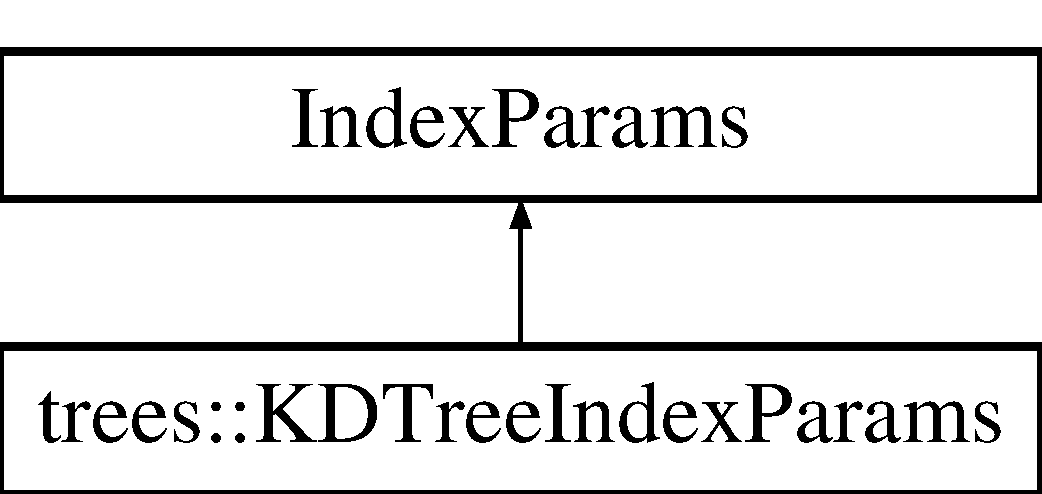
\includegraphics[height=2.000000cm]{structtrees_1_1_k_d_tree_index_params}
\end{center}
\end{figure}
\subsection*{Public Member Functions}
\begin{DoxyCompactItemize}
\item 
\hyperlink{structtrees_1_1_k_d_tree_index_params_a4a1c6e02700c365e787d09fb4b821553}{K\+D\+Tree\+Index\+Params} (int neighbor\+\_\+=30, bool ordered\+\_\+=true)
\end{DoxyCompactItemize}


\subsection{Detailed Description}
Input parameters for the tree 

\subsection{Constructor \& Destructor Documentation}
\mbox{\Hypertarget{structtrees_1_1_k_d_tree_index_params_a4a1c6e02700c365e787d09fb4b821553}\label{structtrees_1_1_k_d_tree_index_params_a4a1c6e02700c365e787d09fb4b821553}} 
\index{trees\+::\+K\+D\+Tree\+Index\+Params@{trees\+::\+K\+D\+Tree\+Index\+Params}!K\+D\+Tree\+Index\+Params@{K\+D\+Tree\+Index\+Params}}
\index{K\+D\+Tree\+Index\+Params@{K\+D\+Tree\+Index\+Params}!trees\+::\+K\+D\+Tree\+Index\+Params@{trees\+::\+K\+D\+Tree\+Index\+Params}}
\subsubsection{\texorpdfstring{K\+D\+Tree\+Index\+Params()}{KDTreeIndexParams()}}
{\footnotesize\ttfamily trees\+::\+K\+D\+Tree\+Index\+Params\+::\+K\+D\+Tree\+Index\+Params (\begin{DoxyParamCaption}\item[{int}]{neighbor\+\_\+ = {\ttfamily 30},  }\item[{bool}]{ordered\+\_\+ = {\ttfamily true} }\end{DoxyParamCaption})\hspace{0.3cm}{\ttfamily [inline]}}

Constructor


\begin{DoxyParams}[1]{Parameters}
\mbox{\tt in}  & {\em neighbor\+\_\+} & Maximal number of neighbors in one node \\
\hline
\mbox{\tt in}  & {\em ordered\+\_\+} & Flag whether th epointcloud shall be sorted \\
\hline
\end{DoxyParams}


The documentation for this struct was generated from the following file\+:\begin{DoxyCompactItemize}
\item 
algorithms/kdtree\+\_\+index.\+h\end{DoxyCompactItemize}

\hypertarget{classtrees_1_1_k_n_n_radius_result_set}{}\section{trees\+:\+:K\+N\+N\+Radius\+Result\+Set$<$ Distance\+Type $>$ Class Template Reference}
\label{classtrees_1_1_k_n_n_radius_result_set}\index{trees\+::\+K\+N\+N\+Radius\+Result\+Set$<$ Distance\+Type $>$@{trees\+::\+K\+N\+N\+Radius\+Result\+Set$<$ Distance\+Type $>$}}


{\ttfamily \#include $<$result\+\_\+set.\+h$>$}

Inheritance diagram for trees\+:\+:K\+N\+N\+Radius\+Result\+Set$<$ Distance\+Type $>$\+:\begin{figure}[H]
\begin{center}
\leavevmode
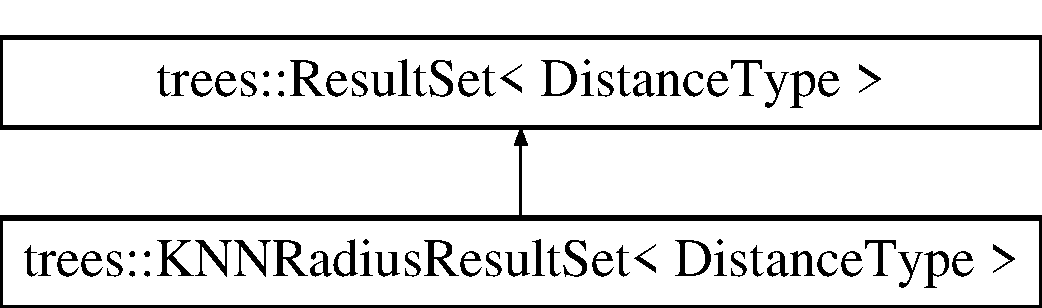
\includegraphics[height=2.000000cm]{classtrees_1_1_k_n_n_radius_result_set}
\end{center}
\end{figure}
\subsection*{Public Types}
\begin{DoxyCompactItemize}
\item 
\mbox{\Hypertarget{classtrees_1_1_k_n_n_radius_result_set_a3fc3b4b132a028361b00884df77f7d7e}\label{classtrees_1_1_k_n_n_radius_result_set_a3fc3b4b132a028361b00884df77f7d7e}} 
typedef \hyperlink{structtrees_1_1_distance_index}{Distance\+Index}$<$ Distance\+Type $>$ {\bfseries Dist\+Index}
\end{DoxyCompactItemize}
\subsection*{Public Member Functions}
\begin{DoxyCompactItemize}
\item 
\mbox{\Hypertarget{classtrees_1_1_k_n_n_radius_result_set_a96bb96f5d6feeda00fafe84cf2458cc9}\label{classtrees_1_1_k_n_n_radius_result_set_a96bb96f5d6feeda00fafe84cf2458cc9}} 
{\bfseries K\+N\+N\+Radius\+Result\+Set} (Distance\+Type radius\+\_\+, size\+\_\+t capacity\+\_\+)
\item 
void \hyperlink{classtrees_1_1_k_n_n_radius_result_set_afc08b678752c4fb938a12a6346a3123f}{clear} ()
\item 
size\+\_\+t \hyperlink{classtrees_1_1_k_n_n_radius_result_set_a3e6a6b74d2dbf9792f4ed632ce4be376}{size} () const
\item 
bool \hyperlink{classtrees_1_1_k_n_n_radius_result_set_aac419c31445e99d3f13830f803c61082}{full} () const
\item 
void \hyperlink{classtrees_1_1_k_n_n_radius_result_set_af19b65b3e39f5ef1715a1d7cb4afc8c5}{add\+Point} (Distance\+Type dist, size\+\_\+t index)
\item 
void \hyperlink{classtrees_1_1_k_n_n_radius_result_set_a2e4e41546c6290f5e0c1d2fcc5845024}{copy} (size\+\_\+t $\ast$indices, Distance\+Type $\ast$dists, size\+\_\+t num\+\_\+elements, bool sorted=true)
\item 
\mbox{\Hypertarget{classtrees_1_1_k_n_n_radius_result_set_a8d2829817802878069fede73816bf78d}\label{classtrees_1_1_k_n_n_radius_result_set_a8d2829817802878069fede73816bf78d}} 
Distance\+Type {\bfseries worst\+Dist} () const
\end{DoxyCompactItemize}
\subsection*{Additional Inherited Members}


\subsection{Detailed Description}
\subsubsection*{template$<$typename Distance\+Type$>$\newline
class trees\+::\+K\+N\+N\+Radius\+Result\+Set$<$ Distance\+Type $>$}

Bounded radius result set. It limits the number of elements it can hold to a preset capacity. 

\subsection{Member Function Documentation}
\mbox{\Hypertarget{classtrees_1_1_k_n_n_radius_result_set_af19b65b3e39f5ef1715a1d7cb4afc8c5}\label{classtrees_1_1_k_n_n_radius_result_set_af19b65b3e39f5ef1715a1d7cb4afc8c5}} 
\index{trees\+::\+K\+N\+N\+Radius\+Result\+Set@{trees\+::\+K\+N\+N\+Radius\+Result\+Set}!add\+Point@{add\+Point}}
\index{add\+Point@{add\+Point}!trees\+::\+K\+N\+N\+Radius\+Result\+Set@{trees\+::\+K\+N\+N\+Radius\+Result\+Set}}
\subsubsection{\texorpdfstring{add\+Point()}{addPoint()}}
{\footnotesize\ttfamily template$<$typename Distance\+Type $>$ \\
void \hyperlink{classtrees_1_1_k_n_n_radius_result_set}{trees\+::\+K\+N\+N\+Radius\+Result\+Set}$<$ Distance\+Type $>$\+::add\+Point (\begin{DoxyParamCaption}\item[{Distance\+Type}]{dist,  }\item[{size\+\_\+t}]{index }\end{DoxyParamCaption})\hspace{0.3cm}{\ttfamily [inline]}, {\ttfamily [virtual]}}

Add another point to result set 
\begin{DoxyParams}{Parameters}
{\em dist} & distance to point \\
\hline
{\em index} & index of point Pre-\/conditions\+: capacity\+\_\+$>$0 \\
\hline
\end{DoxyParams}


Implements \hyperlink{classtrees_1_1_result_set}{trees\+::\+Result\+Set$<$ Distance\+Type $>$}.

\mbox{\Hypertarget{classtrees_1_1_k_n_n_radius_result_set_afc08b678752c4fb938a12a6346a3123f}\label{classtrees_1_1_k_n_n_radius_result_set_afc08b678752c4fb938a12a6346a3123f}} 
\index{trees\+::\+K\+N\+N\+Radius\+Result\+Set@{trees\+::\+K\+N\+N\+Radius\+Result\+Set}!clear@{clear}}
\index{clear@{clear}!trees\+::\+K\+N\+N\+Radius\+Result\+Set@{trees\+::\+K\+N\+N\+Radius\+Result\+Set}}
\subsubsection{\texorpdfstring{clear()}{clear()}}
{\footnotesize\ttfamily template$<$typename Distance\+Type $>$ \\
void \hyperlink{classtrees_1_1_k_n_n_radius_result_set}{trees\+::\+K\+N\+N\+Radius\+Result\+Set}$<$ Distance\+Type $>$\+::clear (\begin{DoxyParamCaption}{ }\end{DoxyParamCaption})\hspace{0.3cm}{\ttfamily [inline]}}

Clears the result set \mbox{\Hypertarget{classtrees_1_1_k_n_n_radius_result_set_a2e4e41546c6290f5e0c1d2fcc5845024}\label{classtrees_1_1_k_n_n_radius_result_set_a2e4e41546c6290f5e0c1d2fcc5845024}} 
\index{trees\+::\+K\+N\+N\+Radius\+Result\+Set@{trees\+::\+K\+N\+N\+Radius\+Result\+Set}!copy@{copy}}
\index{copy@{copy}!trees\+::\+K\+N\+N\+Radius\+Result\+Set@{trees\+::\+K\+N\+N\+Radius\+Result\+Set}}
\subsubsection{\texorpdfstring{copy()}{copy()}}
{\footnotesize\ttfamily template$<$typename Distance\+Type $>$ \\
void \hyperlink{classtrees_1_1_k_n_n_radius_result_set}{trees\+::\+K\+N\+N\+Radius\+Result\+Set}$<$ Distance\+Type $>$\+::copy (\begin{DoxyParamCaption}\item[{size\+\_\+t $\ast$}]{indices,  }\item[{Distance\+Type $\ast$}]{dists,  }\item[{size\+\_\+t}]{num\+\_\+elements,  }\item[{bool}]{sorted = {\ttfamily true} }\end{DoxyParamCaption})\hspace{0.3cm}{\ttfamily [inline]}}

Copy indices and distances to output buffers 
\begin{DoxyParams}{Parameters}
{\em indices} & \\
\hline
{\em dists} & \\
\hline
{\em num\+\_\+elements} & Number of elements to copy \\
\hline
{\em sorted} & Indicates if results should be sorted \\
\hline
\end{DoxyParams}
\mbox{\Hypertarget{classtrees_1_1_k_n_n_radius_result_set_aac419c31445e99d3f13830f803c61082}\label{classtrees_1_1_k_n_n_radius_result_set_aac419c31445e99d3f13830f803c61082}} 
\index{trees\+::\+K\+N\+N\+Radius\+Result\+Set@{trees\+::\+K\+N\+N\+Radius\+Result\+Set}!full@{full}}
\index{full@{full}!trees\+::\+K\+N\+N\+Radius\+Result\+Set@{trees\+::\+K\+N\+N\+Radius\+Result\+Set}}
\subsubsection{\texorpdfstring{full()}{full()}}
{\footnotesize\ttfamily template$<$typename Distance\+Type $>$ \\
bool \hyperlink{classtrees_1_1_k_n_n_radius_result_set}{trees\+::\+K\+N\+N\+Radius\+Result\+Set}$<$ Distance\+Type $>$\+::full (\begin{DoxyParamCaption}{ }\end{DoxyParamCaption}) const\hspace{0.3cm}{\ttfamily [inline]}, {\ttfamily [virtual]}}

Radius search result set always reports full \begin{DoxyReturn}{Returns}

\end{DoxyReturn}


Implements \hyperlink{classtrees_1_1_result_set}{trees\+::\+Result\+Set$<$ Distance\+Type $>$}.

\mbox{\Hypertarget{classtrees_1_1_k_n_n_radius_result_set_a3e6a6b74d2dbf9792f4ed632ce4be376}\label{classtrees_1_1_k_n_n_radius_result_set_a3e6a6b74d2dbf9792f4ed632ce4be376}} 
\index{trees\+::\+K\+N\+N\+Radius\+Result\+Set@{trees\+::\+K\+N\+N\+Radius\+Result\+Set}!size@{size}}
\index{size@{size}!trees\+::\+K\+N\+N\+Radius\+Result\+Set@{trees\+::\+K\+N\+N\+Radius\+Result\+Set}}
\subsubsection{\texorpdfstring{size()}{size()}}
{\footnotesize\ttfamily template$<$typename Distance\+Type $>$ \\
size\+\_\+t \hyperlink{classtrees_1_1_k_n_n_radius_result_set}{trees\+::\+K\+N\+N\+Radius\+Result\+Set}$<$ Distance\+Type $>$\+::size (\begin{DoxyParamCaption}{ }\end{DoxyParamCaption}) const\hspace{0.3cm}{\ttfamily [inline]}}

\begin{DoxyReturn}{Returns}
Number of elements in the result set 
\end{DoxyReturn}


The documentation for this class was generated from the following file\+:\begin{DoxyCompactItemize}
\item 
util/result\+\_\+set.\+h\end{DoxyCompactItemize}

\hypertarget{classtrees_1_1_k_n_n_radius_unique_result_set}{}\section{trees\+:\+:K\+N\+N\+Radius\+Unique\+Result\+Set$<$ Distance\+Type $>$ Class Template Reference}
\label{classtrees_1_1_k_n_n_radius_unique_result_set}\index{trees\+::\+K\+N\+N\+Radius\+Unique\+Result\+Set$<$ Distance\+Type $>$@{trees\+::\+K\+N\+N\+Radius\+Unique\+Result\+Set$<$ Distance\+Type $>$}}


{\ttfamily \#include $<$result\+\_\+set.\+h$>$}

Inheritance diagram for trees\+:\+:K\+N\+N\+Radius\+Unique\+Result\+Set$<$ Distance\+Type $>$\+:\begin{figure}[H]
\begin{center}
\leavevmode
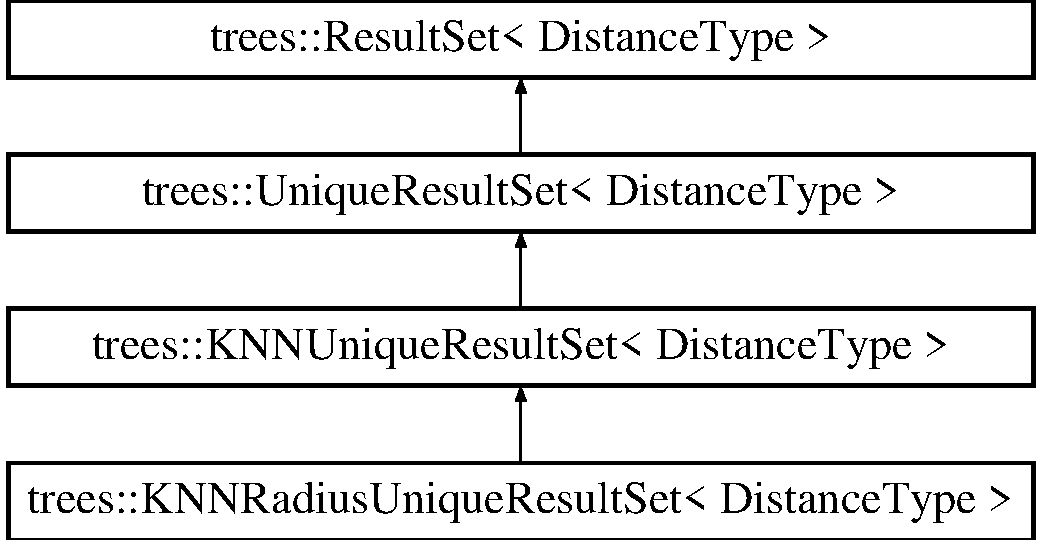
\includegraphics[height=4.000000cm]{classtrees_1_1_k_n_n_radius_unique_result_set}
\end{center}
\end{figure}
\subsection*{Public Member Functions}
\begin{DoxyCompactItemize}
\item 
\hyperlink{classtrees_1_1_k_n_n_radius_unique_result_set_ab20dd750c139d441ab3d715a4b4f1bac}{K\+N\+N\+Radius\+Unique\+Result\+Set} (Distance\+Type radius, size\+\_\+t capacity)
\item 
void \hyperlink{classtrees_1_1_k_n_n_radius_unique_result_set_abf3186df7ed3776c34d824b768975ff9}{clear} ()
\end{DoxyCompactItemize}
\subsection*{Additional Inherited Members}


\subsection{Detailed Description}
\subsubsection*{template$<$typename Distance\+Type$>$\newline
class trees\+::\+K\+N\+N\+Radius\+Unique\+Result\+Set$<$ Distance\+Type $>$}

Class that holds the k NN neighbors within a radius distance 

\subsection{Constructor \& Destructor Documentation}
\mbox{\Hypertarget{classtrees_1_1_k_n_n_radius_unique_result_set_ab20dd750c139d441ab3d715a4b4f1bac}\label{classtrees_1_1_k_n_n_radius_unique_result_set_ab20dd750c139d441ab3d715a4b4f1bac}} 
\index{trees\+::\+K\+N\+N\+Radius\+Unique\+Result\+Set@{trees\+::\+K\+N\+N\+Radius\+Unique\+Result\+Set}!K\+N\+N\+Radius\+Unique\+Result\+Set@{K\+N\+N\+Radius\+Unique\+Result\+Set}}
\index{K\+N\+N\+Radius\+Unique\+Result\+Set@{K\+N\+N\+Radius\+Unique\+Result\+Set}!trees\+::\+K\+N\+N\+Radius\+Unique\+Result\+Set@{trees\+::\+K\+N\+N\+Radius\+Unique\+Result\+Set}}
\subsubsection{\texorpdfstring{K\+N\+N\+Radius\+Unique\+Result\+Set()}{KNNRadiusUniqueResultSet()}}
{\footnotesize\ttfamily template$<$typename Distance\+Type $>$ \\
\hyperlink{classtrees_1_1_k_n_n_radius_unique_result_set}{trees\+::\+K\+N\+N\+Radius\+Unique\+Result\+Set}$<$ Distance\+Type $>$\+::\hyperlink{classtrees_1_1_k_n_n_radius_unique_result_set}{K\+N\+N\+Radius\+Unique\+Result\+Set} (\begin{DoxyParamCaption}\item[{Distance\+Type}]{radius,  }\item[{size\+\_\+t}]{capacity }\end{DoxyParamCaption})\hspace{0.3cm}{\ttfamily [inline]}}

Constructor 
\begin{DoxyParams}{Parameters}
{\em capacity} & the number of neighbors to store at max \\
\hline
\end{DoxyParams}


\subsection{Member Function Documentation}
\mbox{\Hypertarget{classtrees_1_1_k_n_n_radius_unique_result_set_abf3186df7ed3776c34d824b768975ff9}\label{classtrees_1_1_k_n_n_radius_unique_result_set_abf3186df7ed3776c34d824b768975ff9}} 
\index{trees\+::\+K\+N\+N\+Radius\+Unique\+Result\+Set@{trees\+::\+K\+N\+N\+Radius\+Unique\+Result\+Set}!clear@{clear}}
\index{clear@{clear}!trees\+::\+K\+N\+N\+Radius\+Unique\+Result\+Set@{trees\+::\+K\+N\+N\+Radius\+Unique\+Result\+Set}}
\subsubsection{\texorpdfstring{clear()}{clear()}}
{\footnotesize\ttfamily template$<$typename Distance\+Type $>$ \\
void \hyperlink{classtrees_1_1_k_n_n_radius_unique_result_set}{trees\+::\+K\+N\+N\+Radius\+Unique\+Result\+Set}$<$ Distance\+Type $>$\+::clear (\begin{DoxyParamCaption}{ }\end{DoxyParamCaption})\hspace{0.3cm}{\ttfamily [inline]}}

Remove all elements in the set 

The documentation for this class was generated from the following file\+:\begin{DoxyCompactItemize}
\item 
utils/result\+\_\+set.\+h\end{DoxyCompactItemize}

\hypertarget{classtrees_1_1_k_n_n_result_set}{}\section{trees\+:\+:K\+N\+N\+Result\+Set$<$ Distance\+Type $>$ Class Template Reference}
\label{classtrees_1_1_k_n_n_result_set}\index{trees\+::\+K\+N\+N\+Result\+Set$<$ Distance\+Type $>$@{trees\+::\+K\+N\+N\+Result\+Set$<$ Distance\+Type $>$}}


{\ttfamily \#include $<$result\+\_\+set.\+h$>$}

Inheritance diagram for trees\+:\+:K\+N\+N\+Result\+Set$<$ Distance\+Type $>$\+:\begin{figure}[H]
\begin{center}
\leavevmode
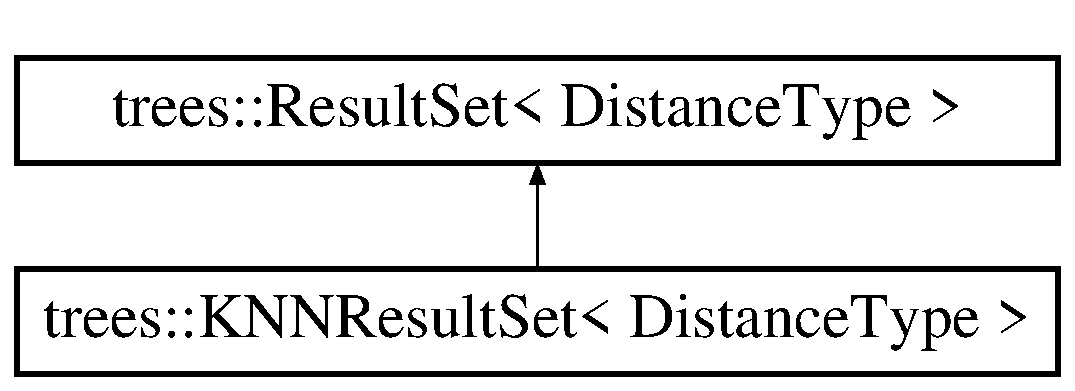
\includegraphics[height=2.000000cm]{classtrees_1_1_k_n_n_result_set}
\end{center}
\end{figure}
\subsection*{Public Types}
\begin{DoxyCompactItemize}
\item 
\mbox{\Hypertarget{classtrees_1_1_k_n_n_result_set_ae243d4e2be3ff92c714898b7fb3b607e}\label{classtrees_1_1_k_n_n_result_set_ae243d4e2be3ff92c714898b7fb3b607e}} 
typedef \hyperlink{structtrees_1_1_distance_index}{Distance\+Index}$<$ Distance\+Type $>$ {\bfseries Dist\+Index}
\end{DoxyCompactItemize}
\subsection*{Public Member Functions}
\begin{DoxyCompactItemize}
\item 
\mbox{\Hypertarget{classtrees_1_1_k_n_n_result_set_af84c8771413e6594b2d63b54797f1ce6}\label{classtrees_1_1_k_n_n_result_set_af84c8771413e6594b2d63b54797f1ce6}} 
{\bfseries K\+N\+N\+Result\+Set} (size\+\_\+t capacity\+\_\+)
\item 
void \hyperlink{classtrees_1_1_k_n_n_result_set_a6faafd1ae6f7dbe5a9fdcf03c244141c}{clear} ()
\item 
\mbox{\Hypertarget{classtrees_1_1_k_n_n_result_set_a3fdf3248d81cfdb9e68b5fc94a46ca38}\label{classtrees_1_1_k_n_n_result_set_a3fdf3248d81cfdb9e68b5fc94a46ca38}} 
size\+\_\+t {\bfseries size} () const
\item 
\mbox{\Hypertarget{classtrees_1_1_k_n_n_result_set_a88d22190d5d32bea60224b55959e336b}\label{classtrees_1_1_k_n_n_result_set_a88d22190d5d32bea60224b55959e336b}} 
bool {\bfseries full} () const
\item 
\mbox{\Hypertarget{classtrees_1_1_k_n_n_result_set_a41aa290d7219ec1e8eca98c04364ba09}\label{classtrees_1_1_k_n_n_result_set_a41aa290d7219ec1e8eca98c04364ba09}} 
void {\bfseries add\+Point} (Distance\+Type dist, size\+\_\+t index)
\item 
void \hyperlink{classtrees_1_1_k_n_n_result_set_a3e1b80d0f5c564f74d840c9838653a39}{copy} (size\+\_\+t $\ast$indices, Distance\+Type $\ast$dists, size\+\_\+t num\+\_\+elements, bool sorted=true)
\item 
\mbox{\Hypertarget{classtrees_1_1_k_n_n_result_set_a684b5be0f09a8ede3cc18e028d4f0e48}\label{classtrees_1_1_k_n_n_result_set_a684b5be0f09a8ede3cc18e028d4f0e48}} 
Distance\+Type {\bfseries worst\+Dist} () const
\end{DoxyCompactItemize}
\subsection*{Additional Inherited Members}


\subsection{Detailed Description}
\subsubsection*{template$<$typename Distance\+Type$>$\newline
class trees\+::\+K\+N\+N\+Result\+Set$<$ Distance\+Type $>$}

K-\/\+Nearest neighbour result set. Ensures that the elements inserted are unique 

\subsection{Member Function Documentation}
\mbox{\Hypertarget{classtrees_1_1_k_n_n_result_set_a6faafd1ae6f7dbe5a9fdcf03c244141c}\label{classtrees_1_1_k_n_n_result_set_a6faafd1ae6f7dbe5a9fdcf03c244141c}} 
\index{trees\+::\+K\+N\+N\+Result\+Set@{trees\+::\+K\+N\+N\+Result\+Set}!clear@{clear}}
\index{clear@{clear}!trees\+::\+K\+N\+N\+Result\+Set@{trees\+::\+K\+N\+N\+Result\+Set}}
\subsubsection{\texorpdfstring{clear()}{clear()}}
{\footnotesize\ttfamily template$<$typename Distance\+Type $>$ \\
void \hyperlink{classtrees_1_1_k_n_n_result_set}{trees\+::\+K\+N\+N\+Result\+Set}$<$ Distance\+Type $>$\+::clear (\begin{DoxyParamCaption}{ }\end{DoxyParamCaption})\hspace{0.3cm}{\ttfamily [inline]}}

Clears the result set \mbox{\Hypertarget{classtrees_1_1_k_n_n_result_set_a3e1b80d0f5c564f74d840c9838653a39}\label{classtrees_1_1_k_n_n_result_set_a3e1b80d0f5c564f74d840c9838653a39}} 
\index{trees\+::\+K\+N\+N\+Result\+Set@{trees\+::\+K\+N\+N\+Result\+Set}!copy@{copy}}
\index{copy@{copy}!trees\+::\+K\+N\+N\+Result\+Set@{trees\+::\+K\+N\+N\+Result\+Set}}
\subsubsection{\texorpdfstring{copy()}{copy()}}
{\footnotesize\ttfamily template$<$typename Distance\+Type $>$ \\
void \hyperlink{classtrees_1_1_k_n_n_result_set}{trees\+::\+K\+N\+N\+Result\+Set}$<$ Distance\+Type $>$\+::copy (\begin{DoxyParamCaption}\item[{size\+\_\+t $\ast$}]{indices,  }\item[{Distance\+Type $\ast$}]{dists,  }\item[{size\+\_\+t}]{num\+\_\+elements,  }\item[{bool}]{sorted = {\ttfamily true} }\end{DoxyParamCaption})\hspace{0.3cm}{\ttfamily [inline]}}

Copy indices and distances to output buffers 
\begin{DoxyParams}{Parameters}
{\em indices} & \\
\hline
{\em dists} & \\
\hline
{\em num\+\_\+elements} & Number of elements to copy \\
\hline
{\em sorted} & Indicates if results should be sorted \\
\hline
\end{DoxyParams}


The documentation for this class was generated from the following file\+:\begin{DoxyCompactItemize}
\item 
utils/result\+\_\+set.\+h\end{DoxyCompactItemize}

\hypertarget{classtrees_1_1_k_n_n_result_set2}{}\section{trees\+:\+:K\+N\+N\+Result\+Set2$<$ Distance\+Type $>$ Class Template Reference}
\label{classtrees_1_1_k_n_n_result_set2}\index{trees\+::\+K\+N\+N\+Result\+Set2$<$ Distance\+Type $>$@{trees\+::\+K\+N\+N\+Result\+Set2$<$ Distance\+Type $>$}}
Inheritance diagram for trees\+:\+:K\+N\+N\+Result\+Set2$<$ Distance\+Type $>$\+:\begin{figure}[H]
\begin{center}
\leavevmode
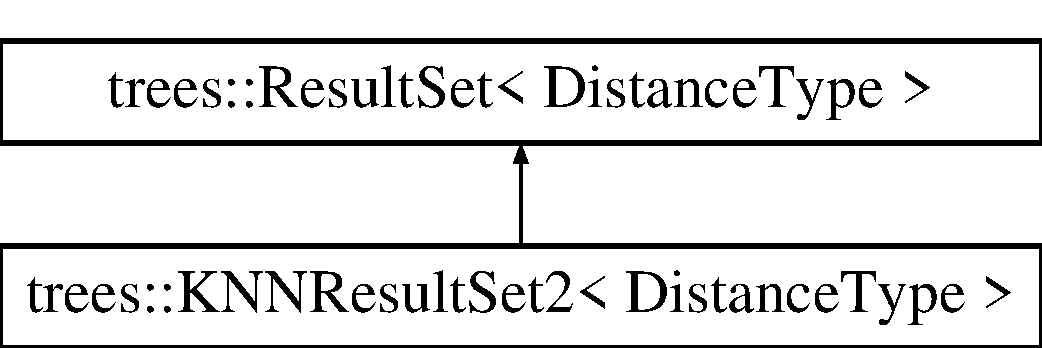
\includegraphics[height=2.000000cm]{classtrees_1_1_k_n_n_result_set2}
\end{center}
\end{figure}
\subsection*{Public Types}
\begin{DoxyCompactItemize}
\item 
\mbox{\Hypertarget{classtrees_1_1_k_n_n_result_set2_a07912021a8df2c09a5a9aa12ae23a28f}\label{classtrees_1_1_k_n_n_result_set2_a07912021a8df2c09a5a9aa12ae23a28f}} 
typedef \hyperlink{structtrees_1_1_distance_index}{Distance\+Index}$<$ Distance\+Type $>$ {\bfseries Dist\+Index}
\end{DoxyCompactItemize}
\subsection*{Public Member Functions}
\begin{DoxyCompactItemize}
\item 
\mbox{\Hypertarget{classtrees_1_1_k_n_n_result_set2_ab87a04c5ee4d4da391452bf4023c100f}\label{classtrees_1_1_k_n_n_result_set2_ab87a04c5ee4d4da391452bf4023c100f}} 
{\bfseries K\+N\+N\+Result\+Set2} (size\+\_\+t capacity\+\_\+)
\item 
void \hyperlink{classtrees_1_1_k_n_n_result_set2_aedf33272f0b7247f3099e37129cf5aaf}{clear} ()
\item 
size\+\_\+t \hyperlink{classtrees_1_1_k_n_n_result_set2_a785fa83af6d1b915443a0b9806c26d82}{size} () const
\item 
bool \hyperlink{classtrees_1_1_k_n_n_result_set2_a903927839600a5871dbecef08002bd29}{full} () const
\item 
void \hyperlink{classtrees_1_1_k_n_n_result_set2_ae67f111b6e4fd6ccdb262552b5881ccc}{add\+Point} (Distance\+Type dist, size\+\_\+t index)
\item 
void \hyperlink{classtrees_1_1_k_n_n_result_set2_aeb8e99886bd18708719c90f22a8d1956}{copy} (size\+\_\+t $\ast$indices, Distance\+Type $\ast$dists, size\+\_\+t num\+\_\+elements, bool sorted=true)
\item 
\mbox{\Hypertarget{classtrees_1_1_k_n_n_result_set2_ae5c43b1692f57f7707310c611baaeb0d}\label{classtrees_1_1_k_n_n_result_set2_ae5c43b1692f57f7707310c611baaeb0d}} 
Distance\+Type {\bfseries worst\+Dist} () const
\end{DoxyCompactItemize}
\subsection*{Additional Inherited Members}


\subsection{Member Function Documentation}
\mbox{\Hypertarget{classtrees_1_1_k_n_n_result_set2_ae67f111b6e4fd6ccdb262552b5881ccc}\label{classtrees_1_1_k_n_n_result_set2_ae67f111b6e4fd6ccdb262552b5881ccc}} 
\index{trees\+::\+K\+N\+N\+Result\+Set2@{trees\+::\+K\+N\+N\+Result\+Set2}!add\+Point@{add\+Point}}
\index{add\+Point@{add\+Point}!trees\+::\+K\+N\+N\+Result\+Set2@{trees\+::\+K\+N\+N\+Result\+Set2}}
\subsubsection{\texorpdfstring{add\+Point()}{addPoint()}}
{\footnotesize\ttfamily template$<$typename Distance\+Type$>$ \\
void \hyperlink{classtrees_1_1_k_n_n_result_set2}{trees\+::\+K\+N\+N\+Result\+Set2}$<$ Distance\+Type $>$\+::add\+Point (\begin{DoxyParamCaption}\item[{Distance\+Type}]{dist,  }\item[{size\+\_\+t}]{index }\end{DoxyParamCaption})\hspace{0.3cm}{\ttfamily [inline]}, {\ttfamily [virtual]}}

Add another point to result set 
\begin{DoxyParams}{Parameters}
{\em dist} & distance to point \\
\hline
{\em index} & index of point Pre-\/conditions\+: capacity\+\_\+$>$0 \\
\hline
\end{DoxyParams}


Implements \hyperlink{classtrees_1_1_result_set}{trees\+::\+Result\+Set$<$ Distance\+Type $>$}.

\mbox{\Hypertarget{classtrees_1_1_k_n_n_result_set2_aedf33272f0b7247f3099e37129cf5aaf}\label{classtrees_1_1_k_n_n_result_set2_aedf33272f0b7247f3099e37129cf5aaf}} 
\index{trees\+::\+K\+N\+N\+Result\+Set2@{trees\+::\+K\+N\+N\+Result\+Set2}!clear@{clear}}
\index{clear@{clear}!trees\+::\+K\+N\+N\+Result\+Set2@{trees\+::\+K\+N\+N\+Result\+Set2}}
\subsubsection{\texorpdfstring{clear()}{clear()}}
{\footnotesize\ttfamily template$<$typename Distance\+Type$>$ \\
void \hyperlink{classtrees_1_1_k_n_n_result_set2}{trees\+::\+K\+N\+N\+Result\+Set2}$<$ Distance\+Type $>$\+::clear (\begin{DoxyParamCaption}{ }\end{DoxyParamCaption})\hspace{0.3cm}{\ttfamily [inline]}}

Clears the result set \mbox{\Hypertarget{classtrees_1_1_k_n_n_result_set2_aeb8e99886bd18708719c90f22a8d1956}\label{classtrees_1_1_k_n_n_result_set2_aeb8e99886bd18708719c90f22a8d1956}} 
\index{trees\+::\+K\+N\+N\+Result\+Set2@{trees\+::\+K\+N\+N\+Result\+Set2}!copy@{copy}}
\index{copy@{copy}!trees\+::\+K\+N\+N\+Result\+Set2@{trees\+::\+K\+N\+N\+Result\+Set2}}
\subsubsection{\texorpdfstring{copy()}{copy()}}
{\footnotesize\ttfamily template$<$typename Distance\+Type$>$ \\
void \hyperlink{classtrees_1_1_k_n_n_result_set2}{trees\+::\+K\+N\+N\+Result\+Set2}$<$ Distance\+Type $>$\+::copy (\begin{DoxyParamCaption}\item[{size\+\_\+t $\ast$}]{indices,  }\item[{Distance\+Type $\ast$}]{dists,  }\item[{size\+\_\+t}]{num\+\_\+elements,  }\item[{bool}]{sorted = {\ttfamily true} }\end{DoxyParamCaption})\hspace{0.3cm}{\ttfamily [inline]}}

Copy indices and distances to output buffers 
\begin{DoxyParams}{Parameters}
{\em indices} & \\
\hline
{\em dists} & \\
\hline
{\em num\+\_\+elements} & Number of elements to copy \\
\hline
{\em sorted} & Indicates if results should be sorted \\
\hline
\end{DoxyParams}
\mbox{\Hypertarget{classtrees_1_1_k_n_n_result_set2_a903927839600a5871dbecef08002bd29}\label{classtrees_1_1_k_n_n_result_set2_a903927839600a5871dbecef08002bd29}} 
\index{trees\+::\+K\+N\+N\+Result\+Set2@{trees\+::\+K\+N\+N\+Result\+Set2}!full@{full}}
\index{full@{full}!trees\+::\+K\+N\+N\+Result\+Set2@{trees\+::\+K\+N\+N\+Result\+Set2}}
\subsubsection{\texorpdfstring{full()}{full()}}
{\footnotesize\ttfamily template$<$typename Distance\+Type$>$ \\
bool \hyperlink{classtrees_1_1_k_n_n_result_set2}{trees\+::\+K\+N\+N\+Result\+Set2}$<$ Distance\+Type $>$\+::full (\begin{DoxyParamCaption}{ }\end{DoxyParamCaption}) const\hspace{0.3cm}{\ttfamily [inline]}, {\ttfamily [virtual]}}

Radius search result set always reports full \begin{DoxyReturn}{Returns}

\end{DoxyReturn}


Implements \hyperlink{classtrees_1_1_result_set}{trees\+::\+Result\+Set$<$ Distance\+Type $>$}.

\mbox{\Hypertarget{classtrees_1_1_k_n_n_result_set2_a785fa83af6d1b915443a0b9806c26d82}\label{classtrees_1_1_k_n_n_result_set2_a785fa83af6d1b915443a0b9806c26d82}} 
\index{trees\+::\+K\+N\+N\+Result\+Set2@{trees\+::\+K\+N\+N\+Result\+Set2}!size@{size}}
\index{size@{size}!trees\+::\+K\+N\+N\+Result\+Set2@{trees\+::\+K\+N\+N\+Result\+Set2}}
\subsubsection{\texorpdfstring{size()}{size()}}
{\footnotesize\ttfamily template$<$typename Distance\+Type$>$ \\
size\+\_\+t \hyperlink{classtrees_1_1_k_n_n_result_set2}{trees\+::\+K\+N\+N\+Result\+Set2}$<$ Distance\+Type $>$\+::size (\begin{DoxyParamCaption}{ }\end{DoxyParamCaption}) const\hspace{0.3cm}{\ttfamily [inline]}}

\begin{DoxyReturn}{Returns}
Number of elements in the result set 
\end{DoxyReturn}


The documentation for this class was generated from the following file\+:\begin{DoxyCompactItemize}
\item 
utils/result\+\_\+set.\+h\end{DoxyCompactItemize}

\hypertarget{classtrees_1_1_k_n_n_simple_result_set}{}\section{trees\+:\+:K\+N\+N\+Simple\+Result\+Set$<$ Distance\+Type $>$ Class Template Reference}
\label{classtrees_1_1_k_n_n_simple_result_set}\index{trees\+::\+K\+N\+N\+Simple\+Result\+Set$<$ Distance\+Type $>$@{trees\+::\+K\+N\+N\+Simple\+Result\+Set$<$ Distance\+Type $>$}}


{\ttfamily \#include $<$result\+\_\+set.\+h$>$}

Inheritance diagram for trees\+:\+:K\+N\+N\+Simple\+Result\+Set$<$ Distance\+Type $>$\+:\begin{figure}[H]
\begin{center}
\leavevmode
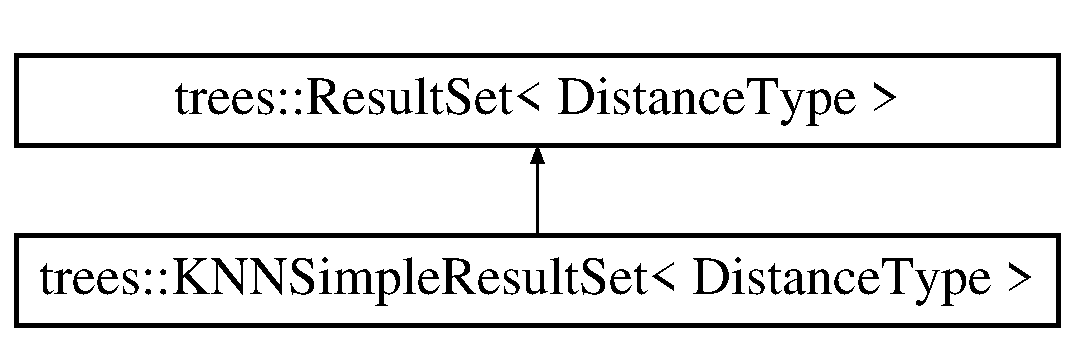
\includegraphics[height=2.000000cm]{classtrees_1_1_k_n_n_simple_result_set}
\end{center}
\end{figure}
\subsection*{Public Types}
\begin{DoxyCompactItemize}
\item 
\mbox{\Hypertarget{classtrees_1_1_k_n_n_simple_result_set_abca1d26dac81173b8e202660b8c8c9f1}\label{classtrees_1_1_k_n_n_simple_result_set_abca1d26dac81173b8e202660b8c8c9f1}} 
typedef \hyperlink{structtrees_1_1_distance_index}{Distance\+Index}$<$ Distance\+Type $>$ {\bfseries Dist\+Index}
\end{DoxyCompactItemize}
\subsection*{Public Member Functions}
\begin{DoxyCompactItemize}
\item 
\mbox{\Hypertarget{classtrees_1_1_k_n_n_simple_result_set_a9b916bba9fe864e42c49a0f402816bd8}\label{classtrees_1_1_k_n_n_simple_result_set_a9b916bba9fe864e42c49a0f402816bd8}} 
{\bfseries K\+N\+N\+Simple\+Result\+Set} (size\+\_\+t capacity\+\_\+)
\item 
void \hyperlink{classtrees_1_1_k_n_n_simple_result_set_a123d8cf8956641841e3b73904414e0b4}{clear} ()
\item 
size\+\_\+t \hyperlink{classtrees_1_1_k_n_n_simple_result_set_a293139927910543164fa430ffdf91311}{size} () const
\item 
bool \hyperlink{classtrees_1_1_k_n_n_simple_result_set_aeaca2d3f888e3abcc4ab4ac5c6eef5d5}{full} () const
\item 
void \hyperlink{classtrees_1_1_k_n_n_simple_result_set_a834254eb4a4e1f4e0046376f9d60719d}{add\+Point} (Distance\+Type dist, size\+\_\+t index)
\item 
void \hyperlink{classtrees_1_1_k_n_n_simple_result_set_aa5ec1079a076f4f989b1af74f11b82fe}{copy} (size\+\_\+t $\ast$indices, Distance\+Type $\ast$dists, size\+\_\+t num\+\_\+elements, bool sorted=true)
\item 
\mbox{\Hypertarget{classtrees_1_1_k_n_n_simple_result_set_a1e1d527fd572a551f8d09d09f81618bf}\label{classtrees_1_1_k_n_n_simple_result_set_a1e1d527fd572a551f8d09d09f81618bf}} 
Distance\+Type {\bfseries worst\+Dist} () const
\end{DoxyCompactItemize}
\subsection*{Additional Inherited Members}


\subsection{Detailed Description}
\subsubsection*{template$<$typename Distance\+Type$>$\newline
class trees\+::\+K\+N\+N\+Simple\+Result\+Set$<$ Distance\+Type $>$}

\hyperlink{classtrees_1_1_k_n_n_simple_result_set}{K\+N\+N\+Simple\+Result\+Set} does not ensure that the element it holds are unique. Is used in those cases where the nearest neighbour algorithm used does not attempt to insert the same element multiple times. 

\subsection{Member Function Documentation}
\mbox{\Hypertarget{classtrees_1_1_k_n_n_simple_result_set_a834254eb4a4e1f4e0046376f9d60719d}\label{classtrees_1_1_k_n_n_simple_result_set_a834254eb4a4e1f4e0046376f9d60719d}} 
\index{trees\+::\+K\+N\+N\+Simple\+Result\+Set@{trees\+::\+K\+N\+N\+Simple\+Result\+Set}!add\+Point@{add\+Point}}
\index{add\+Point@{add\+Point}!trees\+::\+K\+N\+N\+Simple\+Result\+Set@{trees\+::\+K\+N\+N\+Simple\+Result\+Set}}
\subsubsection{\texorpdfstring{add\+Point()}{addPoint()}}
{\footnotesize\ttfamily template$<$typename Distance\+Type $>$ \\
void \hyperlink{classtrees_1_1_k_n_n_simple_result_set}{trees\+::\+K\+N\+N\+Simple\+Result\+Set}$<$ Distance\+Type $>$\+::add\+Point (\begin{DoxyParamCaption}\item[{Distance\+Type}]{dist,  }\item[{size\+\_\+t}]{index }\end{DoxyParamCaption})\hspace{0.3cm}{\ttfamily [inline]}, {\ttfamily [virtual]}}

Add a point to result set 
\begin{DoxyParams}{Parameters}
{\em dist} & distance to point \\
\hline
{\em index} & index of point \\
\hline
\end{DoxyParams}


Implements \hyperlink{classtrees_1_1_result_set}{trees\+::\+Result\+Set$<$ Distance\+Type $>$}.

\mbox{\Hypertarget{classtrees_1_1_k_n_n_simple_result_set_a123d8cf8956641841e3b73904414e0b4}\label{classtrees_1_1_k_n_n_simple_result_set_a123d8cf8956641841e3b73904414e0b4}} 
\index{trees\+::\+K\+N\+N\+Simple\+Result\+Set@{trees\+::\+K\+N\+N\+Simple\+Result\+Set}!clear@{clear}}
\index{clear@{clear}!trees\+::\+K\+N\+N\+Simple\+Result\+Set@{trees\+::\+K\+N\+N\+Simple\+Result\+Set}}
\subsubsection{\texorpdfstring{clear()}{clear()}}
{\footnotesize\ttfamily template$<$typename Distance\+Type $>$ \\
void \hyperlink{classtrees_1_1_k_n_n_simple_result_set}{trees\+::\+K\+N\+N\+Simple\+Result\+Set}$<$ Distance\+Type $>$\+::clear (\begin{DoxyParamCaption}{ }\end{DoxyParamCaption})\hspace{0.3cm}{\ttfamily [inline]}}

Clears the result set \mbox{\Hypertarget{classtrees_1_1_k_n_n_simple_result_set_aa5ec1079a076f4f989b1af74f11b82fe}\label{classtrees_1_1_k_n_n_simple_result_set_aa5ec1079a076f4f989b1af74f11b82fe}} 
\index{trees\+::\+K\+N\+N\+Simple\+Result\+Set@{trees\+::\+K\+N\+N\+Simple\+Result\+Set}!copy@{copy}}
\index{copy@{copy}!trees\+::\+K\+N\+N\+Simple\+Result\+Set@{trees\+::\+K\+N\+N\+Simple\+Result\+Set}}
\subsubsection{\texorpdfstring{copy()}{copy()}}
{\footnotesize\ttfamily template$<$typename Distance\+Type $>$ \\
void \hyperlink{classtrees_1_1_k_n_n_simple_result_set}{trees\+::\+K\+N\+N\+Simple\+Result\+Set}$<$ Distance\+Type $>$\+::copy (\begin{DoxyParamCaption}\item[{size\+\_\+t $\ast$}]{indices,  }\item[{Distance\+Type $\ast$}]{dists,  }\item[{size\+\_\+t}]{num\+\_\+elements,  }\item[{bool}]{sorted = {\ttfamily true} }\end{DoxyParamCaption})\hspace{0.3cm}{\ttfamily [inline]}}

Copy indices and distances to output buffers 
\begin{DoxyParams}{Parameters}
{\em indices} & \\
\hline
{\em dists} & \\
\hline
{\em num\+\_\+elements} & Number of elements to copy \\
\hline
{\em sorted} & Indicates if results should be sorted \\
\hline
\end{DoxyParams}
\mbox{\Hypertarget{classtrees_1_1_k_n_n_simple_result_set_aeaca2d3f888e3abcc4ab4ac5c6eef5d5}\label{classtrees_1_1_k_n_n_simple_result_set_aeaca2d3f888e3abcc4ab4ac5c6eef5d5}} 
\index{trees\+::\+K\+N\+N\+Simple\+Result\+Set@{trees\+::\+K\+N\+N\+Simple\+Result\+Set}!full@{full}}
\index{full@{full}!trees\+::\+K\+N\+N\+Simple\+Result\+Set@{trees\+::\+K\+N\+N\+Simple\+Result\+Set}}
\subsubsection{\texorpdfstring{full()}{full()}}
{\footnotesize\ttfamily template$<$typename Distance\+Type $>$ \\
bool \hyperlink{classtrees_1_1_k_n_n_simple_result_set}{trees\+::\+K\+N\+N\+Simple\+Result\+Set}$<$ Distance\+Type $>$\+::full (\begin{DoxyParamCaption}{ }\end{DoxyParamCaption}) const\hspace{0.3cm}{\ttfamily [inline]}, {\ttfamily [virtual]}}

Radius search result set always reports full \begin{DoxyReturn}{Returns}

\end{DoxyReturn}


Implements \hyperlink{classtrees_1_1_result_set}{trees\+::\+Result\+Set$<$ Distance\+Type $>$}.

\mbox{\Hypertarget{classtrees_1_1_k_n_n_simple_result_set_a293139927910543164fa430ffdf91311}\label{classtrees_1_1_k_n_n_simple_result_set_a293139927910543164fa430ffdf91311}} 
\index{trees\+::\+K\+N\+N\+Simple\+Result\+Set@{trees\+::\+K\+N\+N\+Simple\+Result\+Set}!size@{size}}
\index{size@{size}!trees\+::\+K\+N\+N\+Simple\+Result\+Set@{trees\+::\+K\+N\+N\+Simple\+Result\+Set}}
\subsubsection{\texorpdfstring{size()}{size()}}
{\footnotesize\ttfamily template$<$typename Distance\+Type $>$ \\
size\+\_\+t \hyperlink{classtrees_1_1_k_n_n_simple_result_set}{trees\+::\+K\+N\+N\+Simple\+Result\+Set}$<$ Distance\+Type $>$\+::size (\begin{DoxyParamCaption}{ }\end{DoxyParamCaption}) const\hspace{0.3cm}{\ttfamily [inline]}}

\begin{DoxyReturn}{Returns}
Number of elements in the result set 
\end{DoxyReturn}


The documentation for this class was generated from the following file\+:\begin{DoxyCompactItemize}
\item 
utils/result\+\_\+set.\+h\end{DoxyCompactItemize}

\hypertarget{classtrees_1_1_k_n_n_unique_result_set}{}\section{trees\+:\+:K\+N\+N\+Unique\+Result\+Set$<$ Distance\+Type $>$ Class Template Reference}
\label{classtrees_1_1_k_n_n_unique_result_set}\index{trees\+::\+K\+N\+N\+Unique\+Result\+Set$<$ Distance\+Type $>$@{trees\+::\+K\+N\+N\+Unique\+Result\+Set$<$ Distance\+Type $>$}}


{\ttfamily \#include $<$result\+\_\+set.\+h$>$}

Inheritance diagram for trees\+:\+:K\+N\+N\+Unique\+Result\+Set$<$ Distance\+Type $>$\+:\begin{figure}[H]
\begin{center}
\leavevmode
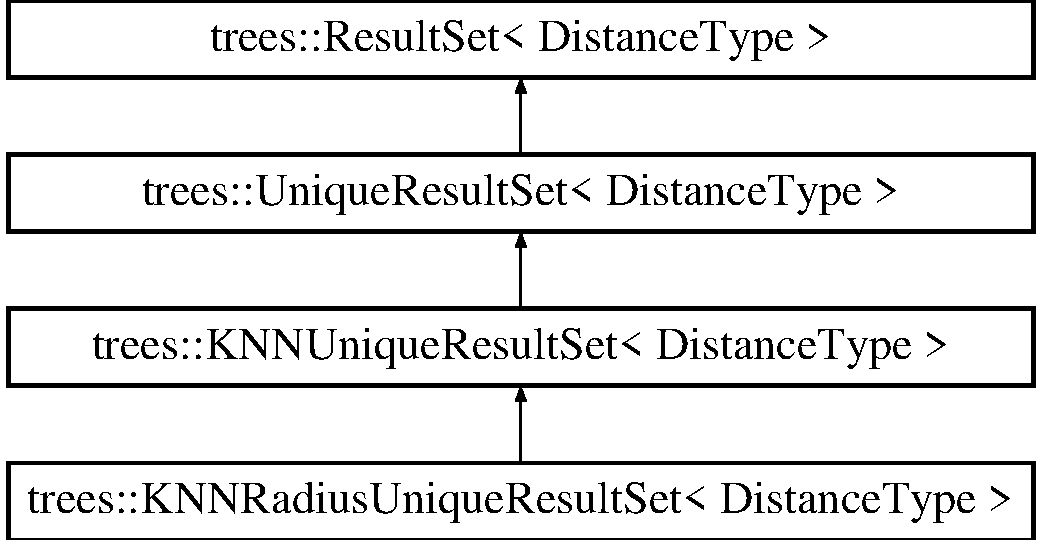
\includegraphics[height=4.000000cm]{classtrees_1_1_k_n_n_unique_result_set}
\end{center}
\end{figure}
\subsection*{Public Member Functions}
\begin{DoxyCompactItemize}
\item 
\hyperlink{classtrees_1_1_k_n_n_unique_result_set_a97620bc6b7febbe8c1885e7191fadf86}{K\+N\+N\+Unique\+Result\+Set} (unsigned int capacity)
\item 
void \hyperlink{classtrees_1_1_k_n_n_unique_result_set_af5525c7d03d3c2f37031b46207aec3a2}{add\+Point} (Distance\+Type dist, size\+\_\+t index)
\item 
void \hyperlink{classtrees_1_1_k_n_n_unique_result_set_aaa6184d20236d8ebe5facb2560751e88}{clear} ()
\end{DoxyCompactItemize}
\subsection*{Protected Types}
\begin{DoxyCompactItemize}
\item 
\mbox{\Hypertarget{classtrees_1_1_k_n_n_unique_result_set_a37696fa83b61266a10aae88a74e534b4}\label{classtrees_1_1_k_n_n_unique_result_set_a37696fa83b61266a10aae88a74e534b4}} 
typedef \hyperlink{classtrees_1_1_unique_result_set}{Unique\+Result\+Set}$<$ Distance\+Type $>$\+::\hyperlink{structtrees_1_1_unique_result_set_1_1_dist_index}{Dist\+Index} {\bfseries Dist\+Index}
\end{DoxyCompactItemize}
\subsection*{Protected Attributes}
\begin{DoxyCompactItemize}
\item 
size\+\_\+t \hyperlink{classtrees_1_1_k_n_n_unique_result_set_a52a3e1ea392eeace263f540865a55250}{capacity\+\_\+}
\end{DoxyCompactItemize}
\subsection*{Additional Inherited Members}


\subsection{Detailed Description}
\subsubsection*{template$<$typename Distance\+Type$>$\newline
class trees\+::\+K\+N\+N\+Unique\+Result\+Set$<$ Distance\+Type $>$}

Class that holds the k NN neighbors Faster than \hyperlink{classtrees_1_1_k_n_n_result_set}{K\+N\+N\+Result\+Set} as it uses a binary heap and does not maintain two arrays 

\subsection{Constructor \& Destructor Documentation}
\mbox{\Hypertarget{classtrees_1_1_k_n_n_unique_result_set_a97620bc6b7febbe8c1885e7191fadf86}\label{classtrees_1_1_k_n_n_unique_result_set_a97620bc6b7febbe8c1885e7191fadf86}} 
\index{trees\+::\+K\+N\+N\+Unique\+Result\+Set@{trees\+::\+K\+N\+N\+Unique\+Result\+Set}!K\+N\+N\+Unique\+Result\+Set@{K\+N\+N\+Unique\+Result\+Set}}
\index{K\+N\+N\+Unique\+Result\+Set@{K\+N\+N\+Unique\+Result\+Set}!trees\+::\+K\+N\+N\+Unique\+Result\+Set@{trees\+::\+K\+N\+N\+Unique\+Result\+Set}}
\subsubsection{\texorpdfstring{K\+N\+N\+Unique\+Result\+Set()}{KNNUniqueResultSet()}}
{\footnotesize\ttfamily template$<$typename Distance\+Type $>$ \\
\hyperlink{classtrees_1_1_k_n_n_unique_result_set}{trees\+::\+K\+N\+N\+Unique\+Result\+Set}$<$ Distance\+Type $>$\+::\hyperlink{classtrees_1_1_k_n_n_unique_result_set}{K\+N\+N\+Unique\+Result\+Set} (\begin{DoxyParamCaption}\item[{unsigned int}]{capacity }\end{DoxyParamCaption})\hspace{0.3cm}{\ttfamily [inline]}}

Constructor 
\begin{DoxyParams}{Parameters}
{\em capacity} & the number of neighbors to store at max \\
\hline
\end{DoxyParams}


\subsection{Member Function Documentation}
\mbox{\Hypertarget{classtrees_1_1_k_n_n_unique_result_set_af5525c7d03d3c2f37031b46207aec3a2}\label{classtrees_1_1_k_n_n_unique_result_set_af5525c7d03d3c2f37031b46207aec3a2}} 
\index{trees\+::\+K\+N\+N\+Unique\+Result\+Set@{trees\+::\+K\+N\+N\+Unique\+Result\+Set}!add\+Point@{add\+Point}}
\index{add\+Point@{add\+Point}!trees\+::\+K\+N\+N\+Unique\+Result\+Set@{trees\+::\+K\+N\+N\+Unique\+Result\+Set}}
\subsubsection{\texorpdfstring{add\+Point()}{addPoint()}}
{\footnotesize\ttfamily template$<$typename Distance\+Type $>$ \\
void \hyperlink{classtrees_1_1_k_n_n_unique_result_set}{trees\+::\+K\+N\+N\+Unique\+Result\+Set}$<$ Distance\+Type $>$\+::add\+Point (\begin{DoxyParamCaption}\item[{Distance\+Type}]{dist,  }\item[{size\+\_\+t}]{index }\end{DoxyParamCaption})\hspace{0.3cm}{\ttfamily [inline]}, {\ttfamily [virtual]}}

Add a possible candidate to the best neighbors 
\begin{DoxyParams}{Parameters}
{\em dist} & distance for that neighbor \\
\hline
{\em index} & index of that neighbor \\
\hline
\end{DoxyParams}


Implements \hyperlink{classtrees_1_1_result_set}{trees\+::\+Result\+Set$<$ Distance\+Type $>$}.

\mbox{\Hypertarget{classtrees_1_1_k_n_n_unique_result_set_aaa6184d20236d8ebe5facb2560751e88}\label{classtrees_1_1_k_n_n_unique_result_set_aaa6184d20236d8ebe5facb2560751e88}} 
\index{trees\+::\+K\+N\+N\+Unique\+Result\+Set@{trees\+::\+K\+N\+N\+Unique\+Result\+Set}!clear@{clear}}
\index{clear@{clear}!trees\+::\+K\+N\+N\+Unique\+Result\+Set@{trees\+::\+K\+N\+N\+Unique\+Result\+Set}}
\subsubsection{\texorpdfstring{clear()}{clear()}}
{\footnotesize\ttfamily template$<$typename Distance\+Type $>$ \\
void \hyperlink{classtrees_1_1_k_n_n_unique_result_set}{trees\+::\+K\+N\+N\+Unique\+Result\+Set}$<$ Distance\+Type $>$\+::clear (\begin{DoxyParamCaption}{ }\end{DoxyParamCaption})\hspace{0.3cm}{\ttfamily [inline]}}

Remove all elements in the set 

\subsection{Member Data Documentation}
\mbox{\Hypertarget{classtrees_1_1_k_n_n_unique_result_set_a52a3e1ea392eeace263f540865a55250}\label{classtrees_1_1_k_n_n_unique_result_set_a52a3e1ea392eeace263f540865a55250}} 
\index{trees\+::\+K\+N\+N\+Unique\+Result\+Set@{trees\+::\+K\+N\+N\+Unique\+Result\+Set}!capacity\+\_\+@{capacity\+\_\+}}
\index{capacity\+\_\+@{capacity\+\_\+}!trees\+::\+K\+N\+N\+Unique\+Result\+Set@{trees\+::\+K\+N\+N\+Unique\+Result\+Set}}
\subsubsection{\texorpdfstring{capacity\+\_\+}{capacity\_}}
{\footnotesize\ttfamily template$<$typename Distance\+Type $>$ \\
size\+\_\+t \hyperlink{classtrees_1_1_k_n_n_unique_result_set}{trees\+::\+K\+N\+N\+Unique\+Result\+Set}$<$ Distance\+Type $>$\+::capacity\+\_\+\hspace{0.3cm}{\ttfamily [protected]}}

The number of neighbors to keep 

The documentation for this class was generated from the following file\+:\begin{DoxyCompactItemize}
\item 
utils/result\+\_\+set.\+h\end{DoxyCompactItemize}

\hypertarget{classtrees_1_1_matrix}{}\section{trees\+:\+:Matrix$<$ Element\+Type $>$ Class Template Reference}
\label{classtrees_1_1_matrix}\index{trees\+::\+Matrix$<$ Element\+Type $>$@{trees\+::\+Matrix$<$ Element\+Type $>$}}
\subsection*{Public Member Functions}
\begin{DoxyCompactItemize}
\item 
\hyperlink{classtrees_1_1_matrix_a363bff5b1ded7ead42eeb72cfee359f3}{Matrix} (void)
\item 
\hyperlink{classtrees_1_1_matrix_a476f805286aeea991d815402c2ff703a}{Matrix} (Element\+Type $\ast$data\+\_\+, size\+\_\+t rows\+\_\+, size\+\_\+t cols\+\_\+)
\item 
\hyperlink{classtrees_1_1_matrix_aaa1772283d722e34a9a914f1d493a754}{Matrix} (const \hyperlink{classtrees_1_1_matrix}{Matrix}$<$ Element\+Type $>$ \&matrix\+\_\+)
\item 
void \hyperlink{classtrees_1_1_matrix_a1467c63bceec8a38771c845fad759784}{operator=} (const \hyperlink{classtrees_1_1_matrix}{Matrix}$<$ Element\+Type $>$ \&matrix\+\_\+)
\item 
\hyperlink{classtrees_1_1_matrix_a4eac26e6570ad219af70aa36eeadc2f7}{$\sim$\+Matrix} ()
\item 
void \hyperlink{classtrees_1_1_matrix_a6911e51830c70251a2655c080f4ad04e}{clear} ()
\item 
Element\+Type $\ast$ \hyperlink{classtrees_1_1_matrix_ae4c759a614daf9f1f019566eca92edab}{get\+Ptr} () const
\item 
Element\+Type $\ast$ \hyperlink{classtrees_1_1_matrix_a8ef252012ddf2ca4ebfd096ff0a1122b}{operator\mbox{[}$\,$\mbox{]}} (size\+\_\+t index\+\_\+) const
\end{DoxyCompactItemize}
\subsection*{Public Attributes}
\begin{DoxyCompactItemize}
\item 
size\+\_\+t \hyperlink{classtrees_1_1_matrix_a88dfff3f217f59caec11e519b23153f6}{rows}
\item 
size\+\_\+t \hyperlink{classtrees_1_1_matrix_a612011a0ae81b3e9d0a7e44a7e827f5c}{cols}
\item 
Element\+Type $\ast$ \hyperlink{classtrees_1_1_matrix_ac7cf0dc5123d2df5cfbac43c5b3c3ee6}{data}
\end{DoxyCompactItemize}


\subsection{Constructor \& Destructor Documentation}
\mbox{\Hypertarget{classtrees_1_1_matrix_a363bff5b1ded7ead42eeb72cfee359f3}\label{classtrees_1_1_matrix_a363bff5b1ded7ead42eeb72cfee359f3}} 
\index{trees\+::\+Matrix@{trees\+::\+Matrix}!Matrix@{Matrix}}
\index{Matrix@{Matrix}!trees\+::\+Matrix@{trees\+::\+Matrix}}
\subsubsection{\texorpdfstring{Matrix()}{Matrix()}\hspace{0.1cm}{\footnotesize\ttfamily [1/3]}}
{\footnotesize\ttfamily template$<$typename Element\+Type$>$ \\
\hyperlink{classtrees_1_1_matrix}{trees\+::\+Matrix}$<$ Element\+Type $>$\+::\hyperlink{classtrees_1_1_matrix}{Matrix} (\begin{DoxyParamCaption}\item[{void}]{ }\end{DoxyParamCaption})\hspace{0.3cm}{\ttfamily [inline]}}

Constructor \mbox{\Hypertarget{classtrees_1_1_matrix_a476f805286aeea991d815402c2ff703a}\label{classtrees_1_1_matrix_a476f805286aeea991d815402c2ff703a}} 
\index{trees\+::\+Matrix@{trees\+::\+Matrix}!Matrix@{Matrix}}
\index{Matrix@{Matrix}!trees\+::\+Matrix@{trees\+::\+Matrix}}
\subsubsection{\texorpdfstring{Matrix()}{Matrix()}\hspace{0.1cm}{\footnotesize\ttfamily [2/3]}}
{\footnotesize\ttfamily template$<$typename Element\+Type$>$ \\
\hyperlink{classtrees_1_1_matrix}{trees\+::\+Matrix}$<$ Element\+Type $>$\+::\hyperlink{classtrees_1_1_matrix}{Matrix} (\begin{DoxyParamCaption}\item[{Element\+Type $\ast$}]{data\+\_\+,  }\item[{size\+\_\+t}]{rows\+\_\+,  }\item[{size\+\_\+t}]{cols\+\_\+ }\end{DoxyParamCaption})\hspace{0.3cm}{\ttfamily [inline]}}

Constructor


\begin{DoxyParams}[1]{Parameters}
\mbox{\tt in}  & {\em data\+\_\+} & Row-\/array of a specific Type \\
\hline
\mbox{\tt in}  & {\em rows\+\_\+} & Rows of the matrix \\
\hline
\mbox{\tt in}  & {\em cols\+\_\+} & Columns of the matrix \\
\hline
\end{DoxyParams}
\mbox{\Hypertarget{classtrees_1_1_matrix_aaa1772283d722e34a9a914f1d493a754}\label{classtrees_1_1_matrix_aaa1772283d722e34a9a914f1d493a754}} 
\index{trees\+::\+Matrix@{trees\+::\+Matrix}!Matrix@{Matrix}}
\index{Matrix@{Matrix}!trees\+::\+Matrix@{trees\+::\+Matrix}}
\subsubsection{\texorpdfstring{Matrix()}{Matrix()}\hspace{0.1cm}{\footnotesize\ttfamily [3/3]}}
{\footnotesize\ttfamily template$<$typename Element\+Type$>$ \\
\hyperlink{classtrees_1_1_matrix}{trees\+::\+Matrix}$<$ Element\+Type $>$\+::\hyperlink{classtrees_1_1_matrix}{Matrix} (\begin{DoxyParamCaption}\item[{const \hyperlink{classtrees_1_1_matrix}{Matrix}$<$ Element\+Type $>$ \&}]{matrix\+\_\+ }\end{DoxyParamCaption})\hspace{0.3cm}{\ttfamily [inline]}}

Copy Constructor


\begin{DoxyParams}[1]{Parameters}
\mbox{\tt in}  & {\em matrix\+\_\+} & \hyperlink{classtrees_1_1_matrix}{Matrix} which shall be copied \\
\hline
\end{DoxyParams}
\mbox{\Hypertarget{classtrees_1_1_matrix_a4eac26e6570ad219af70aa36eeadc2f7}\label{classtrees_1_1_matrix_a4eac26e6570ad219af70aa36eeadc2f7}} 
\index{trees\+::\+Matrix@{trees\+::\+Matrix}!````~Matrix@{$\sim$\+Matrix}}
\index{````~Matrix@{$\sim$\+Matrix}!trees\+::\+Matrix@{trees\+::\+Matrix}}
\subsubsection{\texorpdfstring{$\sim$\+Matrix()}{~Matrix()}}
{\footnotesize\ttfamily template$<$typename Element\+Type$>$ \\
\hyperlink{classtrees_1_1_matrix}{trees\+::\+Matrix}$<$ Element\+Type $>$\+::$\sim$\hyperlink{classtrees_1_1_matrix}{Matrix} (\begin{DoxyParamCaption}{ }\end{DoxyParamCaption})\hspace{0.3cm}{\ttfamily [inline]}}

Deconstructor 

\subsection{Member Function Documentation}
\mbox{\Hypertarget{classtrees_1_1_matrix_a6911e51830c70251a2655c080f4ad04e}\label{classtrees_1_1_matrix_a6911e51830c70251a2655c080f4ad04e}} 
\index{trees\+::\+Matrix@{trees\+::\+Matrix}!clear@{clear}}
\index{clear@{clear}!trees\+::\+Matrix@{trees\+::\+Matrix}}
\subsubsection{\texorpdfstring{clear()}{clear()}}
{\footnotesize\ttfamily template$<$typename Element\+Type$>$ \\
void \hyperlink{classtrees_1_1_matrix}{trees\+::\+Matrix}$<$ Element\+Type $>$\+::clear (\begin{DoxyParamCaption}{ }\end{DoxyParamCaption})\hspace{0.3cm}{\ttfamily [inline]}}

Deletes the data array \mbox{\Hypertarget{classtrees_1_1_matrix_ae4c759a614daf9f1f019566eca92edab}\label{classtrees_1_1_matrix_ae4c759a614daf9f1f019566eca92edab}} 
\index{trees\+::\+Matrix@{trees\+::\+Matrix}!get\+Ptr@{get\+Ptr}}
\index{get\+Ptr@{get\+Ptr}!trees\+::\+Matrix@{trees\+::\+Matrix}}
\subsubsection{\texorpdfstring{get\+Ptr()}{getPtr()}}
{\footnotesize\ttfamily template$<$typename Element\+Type$>$ \\
Element\+Type$\ast$ \hyperlink{classtrees_1_1_matrix}{trees\+::\+Matrix}$<$ Element\+Type $>$\+::get\+Ptr (\begin{DoxyParamCaption}{ }\end{DoxyParamCaption}) const\hspace{0.3cm}{\ttfamily [inline]}}

Returns the pointer of the data array

\begin{DoxyReturn}{Returns}
Return pointer of data array 
\end{DoxyReturn}
\mbox{\Hypertarget{classtrees_1_1_matrix_a1467c63bceec8a38771c845fad759784}\label{classtrees_1_1_matrix_a1467c63bceec8a38771c845fad759784}} 
\index{trees\+::\+Matrix@{trees\+::\+Matrix}!operator=@{operator=}}
\index{operator=@{operator=}!trees\+::\+Matrix@{trees\+::\+Matrix}}
\subsubsection{\texorpdfstring{operator=()}{operator=()}}
{\footnotesize\ttfamily template$<$typename Element\+Type$>$ \\
void \hyperlink{classtrees_1_1_matrix}{trees\+::\+Matrix}$<$ Element\+Type $>$\+::operator= (\begin{DoxyParamCaption}\item[{const \hyperlink{classtrees_1_1_matrix}{Matrix}$<$ Element\+Type $>$ \&}]{matrix\+\_\+ }\end{DoxyParamCaption})\hspace{0.3cm}{\ttfamily [inline]}}

Copy assignment operator


\begin{DoxyParams}[1]{Parameters}
\mbox{\tt in}  & {\em matrix\+\_\+} & \hyperlink{classtrees_1_1_matrix}{Matrix} which shall be copied \\
\hline
\end{DoxyParams}
\mbox{\Hypertarget{classtrees_1_1_matrix_a8ef252012ddf2ca4ebfd096ff0a1122b}\label{classtrees_1_1_matrix_a8ef252012ddf2ca4ebfd096ff0a1122b}} 
\index{trees\+::\+Matrix@{trees\+::\+Matrix}!operator\mbox{[}\mbox{]}@{operator[]}}
\index{operator\mbox{[}\mbox{]}@{operator[]}!trees\+::\+Matrix@{trees\+::\+Matrix}}
\subsubsection{\texorpdfstring{operator[]()}{operator[]()}}
{\footnotesize\ttfamily template$<$typename Element\+Type$>$ \\
Element\+Type$\ast$ \hyperlink{classtrees_1_1_matrix}{trees\+::\+Matrix}$<$ Element\+Type $>$\+::operator\mbox{[}$\,$\mbox{]} (\begin{DoxyParamCaption}\item[{size\+\_\+t}]{index\+\_\+ }\end{DoxyParamCaption}) const\hspace{0.3cm}{\ttfamily [inline]}}

Return the pointer of the indexth row


\begin{DoxyParams}[1]{Parameters}
\mbox{\tt in}  & {\em index\+\_\+} & \hyperlink{classtrees_1_1_index}{Index} of the row \\
\hline
\end{DoxyParams}
\begin{DoxyReturn}{Returns}
Returns the pointer of the indexth row 
\end{DoxyReturn}


\subsection{Member Data Documentation}
\mbox{\Hypertarget{classtrees_1_1_matrix_a612011a0ae81b3e9d0a7e44a7e827f5c}\label{classtrees_1_1_matrix_a612011a0ae81b3e9d0a7e44a7e827f5c}} 
\index{trees\+::\+Matrix@{trees\+::\+Matrix}!cols@{cols}}
\index{cols@{cols}!trees\+::\+Matrix@{trees\+::\+Matrix}}
\subsubsection{\texorpdfstring{cols}{cols}}
{\footnotesize\ttfamily template$<$typename Element\+Type$>$ \\
size\+\_\+t \hyperlink{classtrees_1_1_matrix}{trees\+::\+Matrix}$<$ Element\+Type $>$\+::cols}

Columns of matrix \mbox{\Hypertarget{classtrees_1_1_matrix_ac7cf0dc5123d2df5cfbac43c5b3c3ee6}\label{classtrees_1_1_matrix_ac7cf0dc5123d2df5cfbac43c5b3c3ee6}} 
\index{trees\+::\+Matrix@{trees\+::\+Matrix}!data@{data}}
\index{data@{data}!trees\+::\+Matrix@{trees\+::\+Matrix}}
\subsubsection{\texorpdfstring{data}{data}}
{\footnotesize\ttfamily template$<$typename Element\+Type$>$ \\
Element\+Type$\ast$ \hyperlink{classtrees_1_1_matrix}{trees\+::\+Matrix}$<$ Element\+Type $>$\+::\hyperlink{structdata}{data}}

Pointer to data \mbox{\Hypertarget{classtrees_1_1_matrix_a88dfff3f217f59caec11e519b23153f6}\label{classtrees_1_1_matrix_a88dfff3f217f59caec11e519b23153f6}} 
\index{trees\+::\+Matrix@{trees\+::\+Matrix}!rows@{rows}}
\index{rows@{rows}!trees\+::\+Matrix@{trees\+::\+Matrix}}
\subsubsection{\texorpdfstring{rows}{rows}}
{\footnotesize\ttfamily template$<$typename Element\+Type$>$ \\
size\+\_\+t \hyperlink{classtrees_1_1_matrix}{trees\+::\+Matrix}$<$ Element\+Type $>$\+::rows}

Rows of matrix 

The documentation for this class was generated from the following file\+:\begin{DoxyCompactItemize}
\item 
utils/matrix.\+h\end{DoxyCompactItemize}

\hypertarget{classtrees_1_1_n_n_index}{}\section{trees\+:\+:N\+N\+Index$<$ Element\+Type $>$ Class Template Reference}
\label{classtrees_1_1_n_n_index}\index{trees\+::\+N\+N\+Index$<$ Element\+Type $>$@{trees\+::\+N\+N\+Index$<$ Element\+Type $>$}}
Inheritance diagram for trees\+:\+:N\+N\+Index$<$ Element\+Type $>$\+:\begin{figure}[H]
\begin{center}
\leavevmode
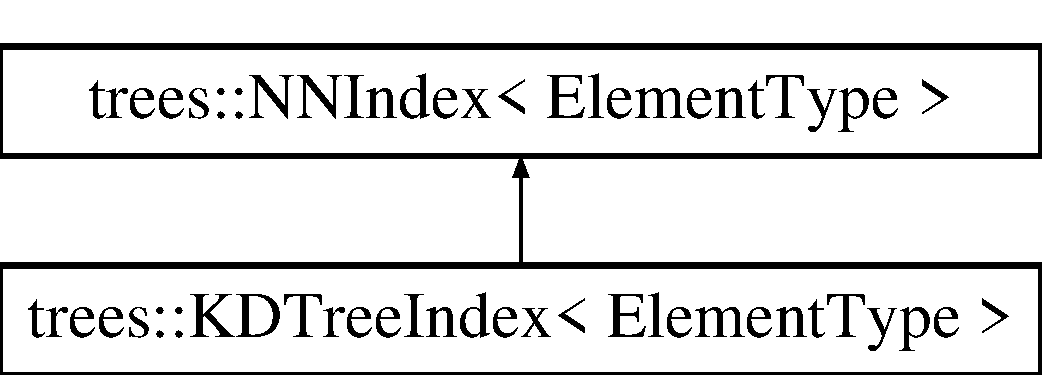
\includegraphics[height=2.000000cm]{classtrees_1_1_n_n_index}
\end{center}
\end{figure}
\subsection*{Public Member Functions}
\begin{DoxyCompactItemize}
\item 
\hyperlink{classtrees_1_1_n_n_index_ae314d8a7c8c0db0eaf22b667b4b4a14e}{N\+N\+Index} ()
\item 
virtual void \hyperlink{classtrees_1_1_n_n_index_afc6b99a8f2693e8b446fc6697dac9f0d}{free\+Index} ()=0
\item 
virtual void \hyperlink{classtrees_1_1_n_n_index_ab209928ad7cf136a482563720d29e2c4}{get\+Dataset} (\hyperlink{classtrees_1_1_matrix}{Matrix}$<$ Element\+Type $>$ \&dataset\+\_\+)=0
\item 
void \hyperlink{classtrees_1_1_n_n_index_a0f02fa0888a3c93b38465ccd37517ba1}{set\+Dataset} (const \hyperlink{classtrees_1_1_matrix}{Matrix}$<$ Element\+Type $>$ \&dataset\+\_\+)
\item 
virtual void \hyperlink{classtrees_1_1_n_n_index_ad8db1182322eba8c1f68ce250e45a36c}{build\+Index} ()
\item 
virtual void \hyperlink{classtrees_1_1_n_n_index_a9efac2e6c3e03ff2cb3f2bd6cacdb3b7}{rebuild} (const \hyperlink{classtrees_1_1_matrix}{Matrix}$<$ Element\+Type $>$ \&dataset\+\_\+)=0
\item 
virtual void \hyperlink{classtrees_1_1_n_n_index_a79c8c1c6ffd00422b97e9df49ff39ec6}{free\+Build} ()=0
\item 
virtual void \hyperlink{classtrees_1_1_n_n_index_a3a280e25b04449f34c4ed0fcc419e7b1}{build\+Index\+Impl} ()=0
\item 
virtual bool \hyperlink{classtrees_1_1_n_n_index_a40d27e58adabc2f21704b9343d85a880}{remove} (size\+\_\+t index\+\_\+)=0
\item 
virtual void \hyperlink{classtrees_1_1_n_n_index_af48da46453e78744d8874c529e06b5ff}{find\+Neighbors} (\hyperlink{classtrees_1_1_result_set}{Result\+Set}$<$ Element\+Type $>$ \&result\+\_\+set\+\_\+, const Element\+Type $\ast$vec\+\_\+, const \hyperlink{structtrees_1_1_tree_params}{Tree\+Params} \&params\+\_\+) const =0
\item 
void \hyperlink{classtrees_1_1_n_n_index_abf4572754ebd83300ab7c7747be10752}{knn\+Search} (const \hyperlink{classtrees_1_1_matrix}{Matrix}$<$ Element\+Type $>$ \&queries\+\_\+, \hyperlink{classtrees_1_1_matrix}{Matrix}$<$ size\+\_\+t $>$ \&indices\+\_\+, \hyperlink{classtrees_1_1_matrix}{Matrix}$<$ Element\+Type $>$ \&dists\+\_\+, size\+\_\+t knn\+\_\+, const \hyperlink{structtrees_1_1_tree_params}{Tree\+Params} \&params\+\_\+)
\item 
void \hyperlink{classtrees_1_1_n_n_index_a059a92d41b77db12a7803e8348ae1c11}{knn\+Search\+Threadpool} (const \hyperlink{classtrees_1_1_matrix}{Matrix}$<$ Element\+Type $>$ \&queries\+\_\+, \hyperlink{classtrees_1_1_matrix}{Matrix}$<$ size\+\_\+t $>$ \&indices\+\_\+, \hyperlink{classtrees_1_1_matrix}{Matrix}$<$ Element\+Type $>$ \&dists\+\_\+, size\+\_\+t knn\+\_\+, const \hyperlink{structtrees_1_1_tree_params}{Tree\+Params} \&params\+\_\+, size\+\_\+t index\+\_\+)
\item 
void \hyperlink{classtrees_1_1_n_n_index_a4f489d7dd35c009a8e1e246dc569f8a0}{knn\+Search} (const \hyperlink{classtrees_1_1_matrix}{Matrix}$<$ Element\+Type $>$ \&queries\+\_\+, \hyperlink{classtrees_1_1_matrix}{Matrix}$<$ int $>$ \&indices\+\_\+, \hyperlink{classtrees_1_1_matrix}{Matrix}$<$ Element\+Type $>$ \&dists\+\_\+, size\+\_\+t knn\+\_\+, const \hyperlink{structtrees_1_1_tree_params}{Tree\+Params} \&params\+\_\+)
\item 
void \hyperlink{classtrees_1_1_n_n_index_ad5227bd07d877a0afee6ac9b7a94177a}{radius\+Search} (const \hyperlink{classtrees_1_1_matrix}{Matrix}$<$ Element\+Type $>$ \&queries\+\_\+, std\+::vector$<$ std\+::vector$<$ size\+\_\+t $>$ $>$ \&indices\+\_\+, std\+::vector$<$ std\+::vector$<$ Element\+Type $>$$>$ \&dists\+\_\+, float radius\+\_\+, const \hyperlink{structtrees_1_1_tree_params}{Tree\+Params} \&params\+\_\+)
\item 
void \hyperlink{classtrees_1_1_n_n_index_af19f1243b64d78dece63fc526fe8307e}{radius\+Search\+Thread} (const \hyperlink{classtrees_1_1_matrix}{Matrix}$<$ Element\+Type $>$ \&queries\+\_\+, std\+::vector$<$ std\+::vector$<$ size\+\_\+t $>$$>$ \&indices\+\_\+, std\+::vector$<$ std\+::vector$<$ Element\+Type $>$$>$ \&dists\+\_\+, float radius\+\_\+, const \hyperlink{structtrees_1_1_tree_params}{Tree\+Params} \&params\+\_\+, size\+\_\+t index\+\_\+)
\item 
void \hyperlink{classtrees_1_1_n_n_index_a2249f50af80e10630f8fb099ffd54acf}{radius\+Search} (const \hyperlink{classtrees_1_1_matrix}{Matrix}$<$ Element\+Type $>$ \&queries\+\_\+, std\+::vector$<$ std\+::vector$<$ int $>$$>$ \&indices\+\_\+, std\+::vector$<$ std\+::vector$<$ Element\+Type $>$$>$ \&dists\+\_\+, float radius\+\_\+, const \hyperlink{structtrees_1_1_tree_params}{Tree\+Params} \&params\+\_\+)
\end{DoxyCompactItemize}
\subsection*{Protected Attributes}
\begin{DoxyCompactItemize}
\item 
size\+\_\+t \hyperlink{classtrees_1_1_n_n_index_a2c14aa447b5461fb839213f092881b23}{size}
\item 
size\+\_\+t \hyperlink{classtrees_1_1_n_n_index_a3da4f85f9618451a8f7d27301fb6ac8c}{veclen}
\item 
\hyperlink{classtrees_1_1_matrix}{Matrix}$<$ Element\+Type $>$ \hyperlink{classtrees_1_1_n_n_index_a895867d67826166ea69def3488847cc6}{dataset}
\end{DoxyCompactItemize}


\subsection{Constructor \& Destructor Documentation}
\mbox{\Hypertarget{classtrees_1_1_n_n_index_ae314d8a7c8c0db0eaf22b667b4b4a14e}\label{classtrees_1_1_n_n_index_ae314d8a7c8c0db0eaf22b667b4b4a14e}} 
\index{trees\+::\+N\+N\+Index@{trees\+::\+N\+N\+Index}!N\+N\+Index@{N\+N\+Index}}
\index{N\+N\+Index@{N\+N\+Index}!trees\+::\+N\+N\+Index@{trees\+::\+N\+N\+Index}}
\subsubsection{\texorpdfstring{N\+N\+Index()}{NNIndex()}}
{\footnotesize\ttfamily template$<$typename Element\+Type$>$ \\
\hyperlink{classtrees_1_1_n_n_index}{trees\+::\+N\+N\+Index}$<$ Element\+Type $>$\+::\hyperlink{classtrees_1_1_n_n_index}{N\+N\+Index} (\begin{DoxyParamCaption}{ }\end{DoxyParamCaption})\hspace{0.3cm}{\ttfamily [inline]}}

Constructor 

\subsection{Member Function Documentation}
\mbox{\Hypertarget{classtrees_1_1_n_n_index_ad8db1182322eba8c1f68ce250e45a36c}\label{classtrees_1_1_n_n_index_ad8db1182322eba8c1f68ce250e45a36c}} 
\index{trees\+::\+N\+N\+Index@{trees\+::\+N\+N\+Index}!build\+Index@{build\+Index}}
\index{build\+Index@{build\+Index}!trees\+::\+N\+N\+Index@{trees\+::\+N\+N\+Index}}
\subsubsection{\texorpdfstring{build\+Index()}{buildIndex()}}
{\footnotesize\ttfamily template$<$typename Element\+Type$>$ \\
virtual void \hyperlink{classtrees_1_1_n_n_index}{trees\+::\+N\+N\+Index}$<$ Element\+Type $>$\+::build\+Index (\begin{DoxyParamCaption}{ }\end{DoxyParamCaption})\hspace{0.3cm}{\ttfamily [inline]}, {\ttfamily [virtual]}}

Build the tree of the specified index \mbox{\Hypertarget{classtrees_1_1_n_n_index_a3a280e25b04449f34c4ed0fcc419e7b1}\label{classtrees_1_1_n_n_index_a3a280e25b04449f34c4ed0fcc419e7b1}} 
\index{trees\+::\+N\+N\+Index@{trees\+::\+N\+N\+Index}!build\+Index\+Impl@{build\+Index\+Impl}}
\index{build\+Index\+Impl@{build\+Index\+Impl}!trees\+::\+N\+N\+Index@{trees\+::\+N\+N\+Index}}
\subsubsection{\texorpdfstring{build\+Index\+Impl()}{buildIndexImpl()}}
{\footnotesize\ttfamily template$<$typename Element\+Type$>$ \\
virtual void \hyperlink{classtrees_1_1_n_n_index}{trees\+::\+N\+N\+Index}$<$ Element\+Type $>$\+::build\+Index\+Impl (\begin{DoxyParamCaption}{ }\end{DoxyParamCaption})\hspace{0.3cm}{\ttfamily [pure virtual]}}

Build the tree of the specified index \mbox{\Hypertarget{classtrees_1_1_n_n_index_af48da46453e78744d8874c529e06b5ff}\label{classtrees_1_1_n_n_index_af48da46453e78744d8874c529e06b5ff}} 
\index{trees\+::\+N\+N\+Index@{trees\+::\+N\+N\+Index}!find\+Neighbors@{find\+Neighbors}}
\index{find\+Neighbors@{find\+Neighbors}!trees\+::\+N\+N\+Index@{trees\+::\+N\+N\+Index}}
\subsubsection{\texorpdfstring{find\+Neighbors()}{findNeighbors()}}
{\footnotesize\ttfamily template$<$typename Element\+Type$>$ \\
virtual void \hyperlink{classtrees_1_1_n_n_index}{trees\+::\+N\+N\+Index}$<$ Element\+Type $>$\+::find\+Neighbors (\begin{DoxyParamCaption}\item[{\hyperlink{classtrees_1_1_result_set}{Result\+Set}$<$ Element\+Type $>$ \&}]{result\+\_\+set\+\_\+,  }\item[{const Element\+Type $\ast$}]{vec\+\_\+,  }\item[{const \hyperlink{structtrees_1_1_tree_params}{Tree\+Params} \&}]{params\+\_\+ }\end{DoxyParamCaption}) const\hspace{0.3cm}{\ttfamily [pure virtual]}}

Prepares the search process, computes initial distances and calls the search function


\begin{DoxyParams}[1]{Parameters}
\mbox{\tt in,out}  & {\em result\+\_\+set\+\_\+} & Container which contains the found neighbors \\
\hline
\mbox{\tt in}  & {\em vec\+\_\+} & Point which neighbors shall be found \\
\hline
\mbox{\tt in}  & {\em params\+\_\+} & Input parameters for the search \\
\hline
\end{DoxyParams}


Implemented in \hyperlink{classtrees_1_1_k_d_tree_index_a37e551977e3c3f772846040819a12e8f}{trees\+::\+K\+D\+Tree\+Index$<$ Element\+Type $>$}.

\mbox{\Hypertarget{classtrees_1_1_n_n_index_a79c8c1c6ffd00422b97e9df49ff39ec6}\label{classtrees_1_1_n_n_index_a79c8c1c6ffd00422b97e9df49ff39ec6}} 
\index{trees\+::\+N\+N\+Index@{trees\+::\+N\+N\+Index}!free\+Build@{free\+Build}}
\index{free\+Build@{free\+Build}!trees\+::\+N\+N\+Index@{trees\+::\+N\+N\+Index}}
\subsubsection{\texorpdfstring{free\+Build()}{freeBuild()}}
{\footnotesize\ttfamily template$<$typename Element\+Type$>$ \\
virtual void \hyperlink{classtrees_1_1_n_n_index}{trees\+::\+N\+N\+Index}$<$ Element\+Type $>$\+::free\+Build (\begin{DoxyParamCaption}{ }\end{DoxyParamCaption})\hspace{0.3cm}{\ttfamily [pure virtual]}}

Free allocated memory for build process \mbox{\Hypertarget{classtrees_1_1_n_n_index_afc6b99a8f2693e8b446fc6697dac9f0d}\label{classtrees_1_1_n_n_index_afc6b99a8f2693e8b446fc6697dac9f0d}} 
\index{trees\+::\+N\+N\+Index@{trees\+::\+N\+N\+Index}!free\+Index@{free\+Index}}
\index{free\+Index@{free\+Index}!trees\+::\+N\+N\+Index@{trees\+::\+N\+N\+Index}}
\subsubsection{\texorpdfstring{free\+Index()}{freeIndex()}}
{\footnotesize\ttfamily template$<$typename Element\+Type$>$ \\
virtual void \hyperlink{classtrees_1_1_n_n_index}{trees\+::\+N\+N\+Index}$<$ Element\+Type $>$\+::free\+Index (\begin{DoxyParamCaption}{ }\end{DoxyParamCaption})\hspace{0.3cm}{\ttfamily [pure virtual]}}

Free allocated memory \mbox{\Hypertarget{classtrees_1_1_n_n_index_ab209928ad7cf136a482563720d29e2c4}\label{classtrees_1_1_n_n_index_ab209928ad7cf136a482563720d29e2c4}} 
\index{trees\+::\+N\+N\+Index@{trees\+::\+N\+N\+Index}!get\+Dataset@{get\+Dataset}}
\index{get\+Dataset@{get\+Dataset}!trees\+::\+N\+N\+Index@{trees\+::\+N\+N\+Index}}
\subsubsection{\texorpdfstring{get\+Dataset()}{getDataset()}}
{\footnotesize\ttfamily template$<$typename Element\+Type$>$ \\
virtual void \hyperlink{classtrees_1_1_n_n_index}{trees\+::\+N\+N\+Index}$<$ Element\+Type $>$\+::get\+Dataset (\begin{DoxyParamCaption}\item[{\hyperlink{classtrees_1_1_matrix}{Matrix}$<$ Element\+Type $>$ \&}]{dataset\+\_\+ }\end{DoxyParamCaption})\hspace{0.3cm}{\ttfamily [pure virtual]}}

Get the dataset \mbox{\Hypertarget{classtrees_1_1_n_n_index_abf4572754ebd83300ab7c7747be10752}\label{classtrees_1_1_n_n_index_abf4572754ebd83300ab7c7747be10752}} 
\index{trees\+::\+N\+N\+Index@{trees\+::\+N\+N\+Index}!knn\+Search@{knn\+Search}}
\index{knn\+Search@{knn\+Search}!trees\+::\+N\+N\+Index@{trees\+::\+N\+N\+Index}}
\subsubsection{\texorpdfstring{knn\+Search()}{knnSearch()}\hspace{0.1cm}{\footnotesize\ttfamily [1/2]}}
{\footnotesize\ttfamily template$<$typename Element\+Type$>$ \\
void \hyperlink{classtrees_1_1_n_n_index}{trees\+::\+N\+N\+Index}$<$ Element\+Type $>$\+::knn\+Search (\begin{DoxyParamCaption}\item[{const \hyperlink{classtrees_1_1_matrix}{Matrix}$<$ Element\+Type $>$ \&}]{queries\+\_\+,  }\item[{\hyperlink{classtrees_1_1_matrix}{Matrix}$<$ size\+\_\+t $>$ \&}]{indices\+\_\+,  }\item[{\hyperlink{classtrees_1_1_matrix}{Matrix}$<$ Element\+Type $>$ \&}]{dists\+\_\+,  }\item[{size\+\_\+t}]{knn\+\_\+,  }\item[{const \hyperlink{structtrees_1_1_tree_params}{Tree\+Params} \&}]{params\+\_\+ }\end{DoxyParamCaption})\hspace{0.3cm}{\ttfamily [inline]}}

Perform k-\/nearest neighbor search


\begin{DoxyParams}[1]{Parameters}
\mbox{\tt in}  & {\em queries\+\_\+} & The query points for which to find the nearest neighbors \\
\hline
\mbox{\tt in,out}  & {\em indices\+\_\+} & The indices of the nearest neighbors found \\
\hline
\mbox{\tt in,out}  & {\em dists\+\_\+} & Distances to the nearest neighbors found \\
\hline
\mbox{\tt in}  & {\em knn\+\_\+} & Number of nearest neighbors to return \\
\hline
\mbox{\tt in}  & {\em params\+\_\+} & Search parameters \\
\hline
\end{DoxyParams}
\mbox{\Hypertarget{classtrees_1_1_n_n_index_a4f489d7dd35c009a8e1e246dc569f8a0}\label{classtrees_1_1_n_n_index_a4f489d7dd35c009a8e1e246dc569f8a0}} 
\index{trees\+::\+N\+N\+Index@{trees\+::\+N\+N\+Index}!knn\+Search@{knn\+Search}}
\index{knn\+Search@{knn\+Search}!trees\+::\+N\+N\+Index@{trees\+::\+N\+N\+Index}}
\subsubsection{\texorpdfstring{knn\+Search()}{knnSearch()}\hspace{0.1cm}{\footnotesize\ttfamily [2/2]}}
{\footnotesize\ttfamily template$<$typename Element\+Type$>$ \\
void \hyperlink{classtrees_1_1_n_n_index}{trees\+::\+N\+N\+Index}$<$ Element\+Type $>$\+::knn\+Search (\begin{DoxyParamCaption}\item[{const \hyperlink{classtrees_1_1_matrix}{Matrix}$<$ Element\+Type $>$ \&}]{queries\+\_\+,  }\item[{\hyperlink{classtrees_1_1_matrix}{Matrix}$<$ int $>$ \&}]{indices\+\_\+,  }\item[{\hyperlink{classtrees_1_1_matrix}{Matrix}$<$ Element\+Type $>$ \&}]{dists\+\_\+,  }\item[{size\+\_\+t}]{knn\+\_\+,  }\item[{const \hyperlink{structtrees_1_1_tree_params}{Tree\+Params} \&}]{params\+\_\+ }\end{DoxyParamCaption})\hspace{0.3cm}{\ttfamily [inline]}}

Perform k-\/nearest neighbor search


\begin{DoxyParams}[1]{Parameters}
\mbox{\tt in}  & {\em queries\+\_\+} & The query points for which to find the nearest neighbors \\
\hline
\mbox{\tt in,out}  & {\em indices\+\_\+} & The indices of the nearest neighbors found \\
\hline
\mbox{\tt in,out}  & {\em dists\+\_\+} & Distances to the nearest neighbors found \\
\hline
\mbox{\tt in}  & {\em knn\+\_\+} & Number of nearest neighbors to return \\
\hline
\mbox{\tt in}  & {\em params\+\_\+} & Search parameters \\
\hline
\end{DoxyParams}
\mbox{\Hypertarget{classtrees_1_1_n_n_index_a059a92d41b77db12a7803e8348ae1c11}\label{classtrees_1_1_n_n_index_a059a92d41b77db12a7803e8348ae1c11}} 
\index{trees\+::\+N\+N\+Index@{trees\+::\+N\+N\+Index}!knn\+Search\+Threadpool@{knn\+Search\+Threadpool}}
\index{knn\+Search\+Threadpool@{knn\+Search\+Threadpool}!trees\+::\+N\+N\+Index@{trees\+::\+N\+N\+Index}}
\subsubsection{\texorpdfstring{knn\+Search\+Threadpool()}{knnSearchThreadpool()}}
{\footnotesize\ttfamily template$<$typename Element\+Type$>$ \\
void \hyperlink{classtrees_1_1_n_n_index}{trees\+::\+N\+N\+Index}$<$ Element\+Type $>$\+::knn\+Search\+Threadpool (\begin{DoxyParamCaption}\item[{const \hyperlink{classtrees_1_1_matrix}{Matrix}$<$ Element\+Type $>$ \&}]{queries\+\_\+,  }\item[{\hyperlink{classtrees_1_1_matrix}{Matrix}$<$ size\+\_\+t $>$ \&}]{indices\+\_\+,  }\item[{\hyperlink{classtrees_1_1_matrix}{Matrix}$<$ Element\+Type $>$ \&}]{dists\+\_\+,  }\item[{size\+\_\+t}]{knn\+\_\+,  }\item[{const \hyperlink{structtrees_1_1_tree_params}{Tree\+Params} \&}]{params\+\_\+,  }\item[{size\+\_\+t}]{index\+\_\+ }\end{DoxyParamCaption})\hspace{0.3cm}{\ttfamily [inline]}}

Perform k-\/nearest neighbor search


\begin{DoxyParams}[1]{Parameters}
\mbox{\tt in}  & {\em queries\+\_\+} & The query points for which to find the nearest neighbors \\
\hline
\mbox{\tt in,out}  & {\em indices\+\_\+} & The indices of the nearest neighbors found \\
\hline
\mbox{\tt in,out}  & {\em dists\+\_\+} & Distances to the nearest neighbors found \\
\hline
\mbox{\tt in}  & {\em knn\+\_\+} & Number of nearest neighbors to return \\
\hline
\mbox{\tt in}  & {\em params\+\_\+} & Search parameters \\
\hline
\mbox{\tt in}  & {\em index\+\_\+} & Number of the row of the queries \\
\hline
\end{DoxyParams}
\mbox{\Hypertarget{classtrees_1_1_n_n_index_ad5227bd07d877a0afee6ac9b7a94177a}\label{classtrees_1_1_n_n_index_ad5227bd07d877a0afee6ac9b7a94177a}} 
\index{trees\+::\+N\+N\+Index@{trees\+::\+N\+N\+Index}!radius\+Search@{radius\+Search}}
\index{radius\+Search@{radius\+Search}!trees\+::\+N\+N\+Index@{trees\+::\+N\+N\+Index}}
\subsubsection{\texorpdfstring{radius\+Search()}{radiusSearch()}\hspace{0.1cm}{\footnotesize\ttfamily [1/2]}}
{\footnotesize\ttfamily template$<$typename Element\+Type$>$ \\
void \hyperlink{classtrees_1_1_n_n_index}{trees\+::\+N\+N\+Index}$<$ Element\+Type $>$\+::radius\+Search (\begin{DoxyParamCaption}\item[{const \hyperlink{classtrees_1_1_matrix}{Matrix}$<$ Element\+Type $>$ \&}]{queries\+\_\+,  }\item[{std\+::vector$<$ std\+::vector$<$ size\+\_\+t $>$ $>$ \&}]{indices\+\_\+,  }\item[{std\+::vector$<$ std\+::vector$<$ Element\+Type $>$$>$ \&}]{dists\+\_\+,  }\item[{float}]{radius\+\_\+,  }\item[{const \hyperlink{structtrees_1_1_tree_params}{Tree\+Params} \&}]{params\+\_\+ }\end{DoxyParamCaption})\hspace{0.3cm}{\ttfamily [inline]}}

Perform radius search


\begin{DoxyParams}[1]{Parameters}
\mbox{\tt in}  & {\em queries\+\_\+} & The query points for which to find the nearest neighbors \\
\hline
\mbox{\tt in,out}  & {\em indices\+\_\+} & The indices of the nearest neighbors found \\
\hline
\mbox{\tt in,out}  & {\em dists\+\_\+} & Distances to the nearest neighbors found \\
\hline
\mbox{\tt in}  & {\em radius\+\_\+} & The radius used for search \\
\hline
\mbox{\tt in}  & {\em params\+\_\+} & Search parameters \\
\hline
\end{DoxyParams}
\mbox{\Hypertarget{classtrees_1_1_n_n_index_a2249f50af80e10630f8fb099ffd54acf}\label{classtrees_1_1_n_n_index_a2249f50af80e10630f8fb099ffd54acf}} 
\index{trees\+::\+N\+N\+Index@{trees\+::\+N\+N\+Index}!radius\+Search@{radius\+Search}}
\index{radius\+Search@{radius\+Search}!trees\+::\+N\+N\+Index@{trees\+::\+N\+N\+Index}}
\subsubsection{\texorpdfstring{radius\+Search()}{radiusSearch()}\hspace{0.1cm}{\footnotesize\ttfamily [2/2]}}
{\footnotesize\ttfamily template$<$typename Element\+Type$>$ \\
void \hyperlink{classtrees_1_1_n_n_index}{trees\+::\+N\+N\+Index}$<$ Element\+Type $>$\+::radius\+Search (\begin{DoxyParamCaption}\item[{const \hyperlink{classtrees_1_1_matrix}{Matrix}$<$ Element\+Type $>$ \&}]{queries\+\_\+,  }\item[{std\+::vector$<$ std\+::vector$<$ int $>$$>$ \&}]{indices\+\_\+,  }\item[{std\+::vector$<$ std\+::vector$<$ Element\+Type $>$$>$ \&}]{dists\+\_\+,  }\item[{float}]{radius\+\_\+,  }\item[{const \hyperlink{structtrees_1_1_tree_params}{Tree\+Params} \&}]{params\+\_\+ }\end{DoxyParamCaption})\hspace{0.3cm}{\ttfamily [inline]}}

Perform radius search


\begin{DoxyParams}[1]{Parameters}
\mbox{\tt in}  & {\em queries\+\_\+} & The query points for which to find the nearest neighbors \\
\hline
\mbox{\tt in,out}  & {\em indices\+\_\+} & The indices of the nearest neighbors found \\
\hline
\mbox{\tt in,out}  & {\em dists\+\_\+} & Distances to the nearest neighbors found \\
\hline
\mbox{\tt in}  & {\em radius\+\_\+} & The radius used for search \\
\hline
\mbox{\tt in}  & {\em params\+\_\+} & Search parameters \\
\hline
\end{DoxyParams}
\mbox{\Hypertarget{classtrees_1_1_n_n_index_af19f1243b64d78dece63fc526fe8307e}\label{classtrees_1_1_n_n_index_af19f1243b64d78dece63fc526fe8307e}} 
\index{trees\+::\+N\+N\+Index@{trees\+::\+N\+N\+Index}!radius\+Search\+Thread@{radius\+Search\+Thread}}
\index{radius\+Search\+Thread@{radius\+Search\+Thread}!trees\+::\+N\+N\+Index@{trees\+::\+N\+N\+Index}}
\subsubsection{\texorpdfstring{radius\+Search\+Thread()}{radiusSearchThread()}}
{\footnotesize\ttfamily template$<$typename Element\+Type$>$ \\
void \hyperlink{classtrees_1_1_n_n_index}{trees\+::\+N\+N\+Index}$<$ Element\+Type $>$\+::radius\+Search\+Thread (\begin{DoxyParamCaption}\item[{const \hyperlink{classtrees_1_1_matrix}{Matrix}$<$ Element\+Type $>$ \&}]{queries\+\_\+,  }\item[{std\+::vector$<$ std\+::vector$<$ size\+\_\+t $>$$>$ \&}]{indices\+\_\+,  }\item[{std\+::vector$<$ std\+::vector$<$ Element\+Type $>$$>$ \&}]{dists\+\_\+,  }\item[{float}]{radius\+\_\+,  }\item[{const \hyperlink{structtrees_1_1_tree_params}{Tree\+Params} \&}]{params\+\_\+,  }\item[{size\+\_\+t}]{index\+\_\+ }\end{DoxyParamCaption})\hspace{0.3cm}{\ttfamily [inline]}}

Perform radius search


\begin{DoxyParams}[1]{Parameters}
\mbox{\tt in}  & {\em queries\+\_\+} & The query points for which to find the nearest neighbors \\
\hline
\mbox{\tt in,out}  & {\em indices\+\_\+} & The indices of the nearest neighbors found \\
\hline
\mbox{\tt in,out}  & {\em dists\+\_\+} & Distances to the nearest neighbors found \\
\hline
\mbox{\tt in}  & {\em radius\+\_\+} & The radius used for search \\
\hline
\mbox{\tt in}  & {\em params\+\_\+} & Search parameters \\
\hline
\mbox{\tt in}  & {\em index\+\_\+} & Number of the row of the queries \\
\hline
\end{DoxyParams}
\mbox{\Hypertarget{classtrees_1_1_n_n_index_a9efac2e6c3e03ff2cb3f2bd6cacdb3b7}\label{classtrees_1_1_n_n_index_a9efac2e6c3e03ff2cb3f2bd6cacdb3b7}} 
\index{trees\+::\+N\+N\+Index@{trees\+::\+N\+N\+Index}!rebuild@{rebuild}}
\index{rebuild@{rebuild}!trees\+::\+N\+N\+Index@{trees\+::\+N\+N\+Index}}
\subsubsection{\texorpdfstring{rebuild()}{rebuild()}}
{\footnotesize\ttfamily template$<$typename Element\+Type$>$ \\
virtual void \hyperlink{classtrees_1_1_n_n_index}{trees\+::\+N\+N\+Index}$<$ Element\+Type $>$\+::rebuild (\begin{DoxyParamCaption}\item[{const \hyperlink{classtrees_1_1_matrix}{Matrix}$<$ Element\+Type $>$ \&}]{dataset\+\_\+ }\end{DoxyParamCaption})\hspace{0.3cm}{\ttfamily [pure virtual]}}

Rebuilds the index


\begin{DoxyParams}[1]{Parameters}
\mbox{\tt in}  & {\em dataset\+\_\+} & Pointcloud \\
\hline
\end{DoxyParams}
\mbox{\Hypertarget{classtrees_1_1_n_n_index_a40d27e58adabc2f21704b9343d85a880}\label{classtrees_1_1_n_n_index_a40d27e58adabc2f21704b9343d85a880}} 
\index{trees\+::\+N\+N\+Index@{trees\+::\+N\+N\+Index}!remove@{remove}}
\index{remove@{remove}!trees\+::\+N\+N\+Index@{trees\+::\+N\+N\+Index}}
\subsubsection{\texorpdfstring{remove()}{remove()}}
{\footnotesize\ttfamily template$<$typename Element\+Type$>$ \\
virtual bool \hyperlink{classtrees_1_1_n_n_index}{trees\+::\+N\+N\+Index}$<$ Element\+Type $>$\+::remove (\begin{DoxyParamCaption}\item[{size\+\_\+t}]{index\+\_\+ }\end{DoxyParamCaption})\hspace{0.3cm}{\ttfamily [pure virtual]}}

Removes point from kdtree


\begin{DoxyParams}[1]{Parameters}
\mbox{\tt in}  & {\em index\+\_\+} & \hyperlink{classtrees_1_1_index}{Index} of the point in the pointcloud \\
\hline
\end{DoxyParams}
\mbox{\Hypertarget{classtrees_1_1_n_n_index_a0f02fa0888a3c93b38465ccd37517ba1}\label{classtrees_1_1_n_n_index_a0f02fa0888a3c93b38465ccd37517ba1}} 
\index{trees\+::\+N\+N\+Index@{trees\+::\+N\+N\+Index}!set\+Dataset@{set\+Dataset}}
\index{set\+Dataset@{set\+Dataset}!trees\+::\+N\+N\+Index@{trees\+::\+N\+N\+Index}}
\subsubsection{\texorpdfstring{set\+Dataset()}{setDataset()}}
{\footnotesize\ttfamily template$<$typename Element\+Type$>$ \\
void \hyperlink{classtrees_1_1_n_n_index}{trees\+::\+N\+N\+Index}$<$ Element\+Type $>$\+::set\+Dataset (\begin{DoxyParamCaption}\item[{const \hyperlink{classtrees_1_1_matrix}{Matrix}$<$ Element\+Type $>$ \&}]{dataset\+\_\+ }\end{DoxyParamCaption})\hspace{0.3cm}{\ttfamily [inline]}}

Set parameters based on the input pointcloud


\begin{DoxyParams}[1]{Parameters}
\mbox{\tt in}  & {\em dataset\+\_\+} & Pointcloud \\
\hline
\end{DoxyParams}


\subsection{Member Data Documentation}
\mbox{\Hypertarget{classtrees_1_1_n_n_index_a895867d67826166ea69def3488847cc6}\label{classtrees_1_1_n_n_index_a895867d67826166ea69def3488847cc6}} 
\index{trees\+::\+N\+N\+Index@{trees\+::\+N\+N\+Index}!dataset@{dataset}}
\index{dataset@{dataset}!trees\+::\+N\+N\+Index@{trees\+::\+N\+N\+Index}}
\subsubsection{\texorpdfstring{dataset}{dataset}}
{\footnotesize\ttfamily template$<$typename Element\+Type$>$ \\
\hyperlink{classtrees_1_1_matrix}{Matrix}$<$Element\+Type$>$ \hyperlink{classtrees_1_1_n_n_index}{trees\+::\+N\+N\+Index}$<$ Element\+Type $>$\+::dataset\hspace{0.3cm}{\ttfamily [protected]}}

Pointcloud \mbox{\Hypertarget{classtrees_1_1_n_n_index_a2c14aa447b5461fb839213f092881b23}\label{classtrees_1_1_n_n_index_a2c14aa447b5461fb839213f092881b23}} 
\index{trees\+::\+N\+N\+Index@{trees\+::\+N\+N\+Index}!size@{size}}
\index{size@{size}!trees\+::\+N\+N\+Index@{trees\+::\+N\+N\+Index}}
\subsubsection{\texorpdfstring{size}{size}}
{\footnotesize\ttfamily template$<$typename Element\+Type$>$ \\
size\+\_\+t \hyperlink{classtrees_1_1_n_n_index}{trees\+::\+N\+N\+Index}$<$ Element\+Type $>$\+::size\hspace{0.3cm}{\ttfamily [protected]}}

Numbers of points in pointcloud \mbox{\Hypertarget{classtrees_1_1_n_n_index_a3da4f85f9618451a8f7d27301fb6ac8c}\label{classtrees_1_1_n_n_index_a3da4f85f9618451a8f7d27301fb6ac8c}} 
\index{trees\+::\+N\+N\+Index@{trees\+::\+N\+N\+Index}!veclen@{veclen}}
\index{veclen@{veclen}!trees\+::\+N\+N\+Index@{trees\+::\+N\+N\+Index}}
\subsubsection{\texorpdfstring{veclen}{veclen}}
{\footnotesize\ttfamily template$<$typename Element\+Type$>$ \\
size\+\_\+t \hyperlink{classtrees_1_1_n_n_index}{trees\+::\+N\+N\+Index}$<$ Element\+Type $>$\+::veclen\hspace{0.3cm}{\ttfamily [protected]}}

Number of dimensions of data 

The documentation for this class was generated from the following file\+:\begin{DoxyCompactItemize}
\item 
algorithms/nn\+\_\+index.\+h\end{DoxyCompactItemize}

\hypertarget{structtrees_1_1_k_d_tree_index_1_1_node}{}\section{trees\+:\+:K\+D\+Tree\+Index$<$ Element\+Type $>$\+:\+:Node Struct Reference}
\label{structtrees_1_1_k_d_tree_index_1_1_node}\index{trees\+::\+K\+D\+Tree\+Index$<$ Element\+Type $>$\+::\+Node@{trees\+::\+K\+D\+Tree\+Index$<$ Element\+Type $>$\+::\+Node}}


{\ttfamily \#include $<$kdtree\+\_\+index.\+h$>$}

\subsection*{Public Attributes}
\begin{DoxyCompactItemize}
\item 
int \hyperlink{structtrees_1_1_k_d_tree_index_1_1_node_aae063499d92e644cfc075f9c151b185b}{left}
\item 
\mbox{\Hypertarget{structtrees_1_1_k_d_tree_index_1_1_node_a601b2967dc00c2c31217edf6d00a4edc}\label{structtrees_1_1_k_d_tree_index_1_1_node_a601b2967dc00c2c31217edf6d00a4edc}} 
int {\bfseries right}
\item 
int \hyperlink{structtrees_1_1_k_d_tree_index_1_1_node_a74e21eb4490a4c6096de83affb7a4867}{divfeat}
\item 
Element\+Type \hyperlink{structtrees_1_1_k_d_tree_index_1_1_node_aa80b732e6a6da3c9d43b09efdf949a06}{divlow}
\item 
\mbox{\Hypertarget{structtrees_1_1_k_d_tree_index_1_1_node_a8b613dd555800178d8cc871a3bf39b85}\label{structtrees_1_1_k_d_tree_index_1_1_node_a8b613dd555800178d8cc871a3bf39b85}} 
Element\+Type {\bfseries divhigh}
\item 
\hyperlink{structtrees_1_1_k_d_tree_index_1_1_node}{Node} $\ast$ \hyperlink{structtrees_1_1_k_d_tree_index_1_1_node_aa210b66e05f8a061872e46893dbb614e}{child1}
\item 
\mbox{\Hypertarget{structtrees_1_1_k_d_tree_index_1_1_node_ade8a4b109317e4059ee99f89aad390dd}\label{structtrees_1_1_k_d_tree_index_1_1_node_ade8a4b109317e4059ee99f89aad390dd}} 
\hyperlink{structtrees_1_1_k_d_tree_index_1_1_node}{Node} $\ast$ {\bfseries child2}
\item 
\hyperlink{structtrees_1_1_k_d_tree_index_1_1_node}{Node} $\ast$ \hyperlink{structtrees_1_1_k_d_tree_index_1_1_node_a987f89ac48760137312cf2aca0ca8b14}{parent}
\end{DoxyCompactItemize}


\subsection{Detailed Description}
\subsubsection*{template$<$typename Element\+Type$>$\newline
struct trees\+::\+K\+D\+Tree\+Index$<$ Element\+Type $>$\+::\+Node}

Structure for a node in the tree 

\subsection{Member Data Documentation}
\mbox{\Hypertarget{structtrees_1_1_k_d_tree_index_1_1_node_aa210b66e05f8a061872e46893dbb614e}\label{structtrees_1_1_k_d_tree_index_1_1_node_aa210b66e05f8a061872e46893dbb614e}} 
\index{trees\+::\+K\+D\+Tree\+Index\+::\+Node@{trees\+::\+K\+D\+Tree\+Index\+::\+Node}!child1@{child1}}
\index{child1@{child1}!trees\+::\+K\+D\+Tree\+Index\+::\+Node@{trees\+::\+K\+D\+Tree\+Index\+::\+Node}}
\subsubsection{\texorpdfstring{child1}{child1}}
{\footnotesize\ttfamily template$<$typename Element\+Type $>$ \\
\hyperlink{structtrees_1_1_k_d_tree_index_1_1_node}{Node}$\ast$ \hyperlink{classtrees_1_1_k_d_tree_index}{trees\+::\+K\+D\+Tree\+Index}$<$ Element\+Type $>$\+::Node\+::child1}

The child nodes \mbox{\Hypertarget{structtrees_1_1_k_d_tree_index_1_1_node_a74e21eb4490a4c6096de83affb7a4867}\label{structtrees_1_1_k_d_tree_index_1_1_node_a74e21eb4490a4c6096de83affb7a4867}} 
\index{trees\+::\+K\+D\+Tree\+Index\+::\+Node@{trees\+::\+K\+D\+Tree\+Index\+::\+Node}!divfeat@{divfeat}}
\index{divfeat@{divfeat}!trees\+::\+K\+D\+Tree\+Index\+::\+Node@{trees\+::\+K\+D\+Tree\+Index\+::\+Node}}
\subsubsection{\texorpdfstring{divfeat}{divfeat}}
{\footnotesize\ttfamily template$<$typename Element\+Type $>$ \\
int \hyperlink{classtrees_1_1_k_d_tree_index}{trees\+::\+K\+D\+Tree\+Index}$<$ Element\+Type $>$\+::Node\+::divfeat}

Dimension used for subdivision \mbox{\Hypertarget{structtrees_1_1_k_d_tree_index_1_1_node_aa80b732e6a6da3c9d43b09efdf949a06}\label{structtrees_1_1_k_d_tree_index_1_1_node_aa80b732e6a6da3c9d43b09efdf949a06}} 
\index{trees\+::\+K\+D\+Tree\+Index\+::\+Node@{trees\+::\+K\+D\+Tree\+Index\+::\+Node}!divlow@{divlow}}
\index{divlow@{divlow}!trees\+::\+K\+D\+Tree\+Index\+::\+Node@{trees\+::\+K\+D\+Tree\+Index\+::\+Node}}
\subsubsection{\texorpdfstring{divlow}{divlow}}
{\footnotesize\ttfamily template$<$typename Element\+Type $>$ \\
Element\+Type \hyperlink{classtrees_1_1_k_d_tree_index}{trees\+::\+K\+D\+Tree\+Index}$<$ Element\+Type $>$\+::Node\+::divlow}

The values used for subdivision \mbox{\Hypertarget{structtrees_1_1_k_d_tree_index_1_1_node_aae063499d92e644cfc075f9c151b185b}\label{structtrees_1_1_k_d_tree_index_1_1_node_aae063499d92e644cfc075f9c151b185b}} 
\index{trees\+::\+K\+D\+Tree\+Index\+::\+Node@{trees\+::\+K\+D\+Tree\+Index\+::\+Node}!left@{left}}
\index{left@{left}!trees\+::\+K\+D\+Tree\+Index\+::\+Node@{trees\+::\+K\+D\+Tree\+Index\+::\+Node}}
\subsubsection{\texorpdfstring{left}{left}}
{\footnotesize\ttfamily template$<$typename Element\+Type $>$ \\
int \hyperlink{classtrees_1_1_k_d_tree_index}{trees\+::\+K\+D\+Tree\+Index}$<$ Element\+Type $>$\+::Node\+::left}

Indices of points in leaf node \mbox{\Hypertarget{structtrees_1_1_k_d_tree_index_1_1_node_a987f89ac48760137312cf2aca0ca8b14}\label{structtrees_1_1_k_d_tree_index_1_1_node_a987f89ac48760137312cf2aca0ca8b14}} 
\index{trees\+::\+K\+D\+Tree\+Index\+::\+Node@{trees\+::\+K\+D\+Tree\+Index\+::\+Node}!parent@{parent}}
\index{parent@{parent}!trees\+::\+K\+D\+Tree\+Index\+::\+Node@{trees\+::\+K\+D\+Tree\+Index\+::\+Node}}
\subsubsection{\texorpdfstring{parent}{parent}}
{\footnotesize\ttfamily template$<$typename Element\+Type $>$ \\
\hyperlink{structtrees_1_1_k_d_tree_index_1_1_node}{Node}$\ast$ \hyperlink{classtrees_1_1_k_d_tree_index}{trees\+::\+K\+D\+Tree\+Index}$<$ Element\+Type $>$\+::Node\+::parent}

Parent 

The documentation for this struct was generated from the following file\+:\begin{DoxyCompactItemize}
\item 
algorithms/kdtree\+\_\+index.\+h\end{DoxyCompactItemize}

\hypertarget{classtrees_1_1_pooled_allocator}{}\section{trees\+:\+:Pooled\+Allocator Class Reference}
\label{classtrees_1_1_pooled_allocator}\index{trees\+::\+Pooled\+Allocator@{trees\+::\+Pooled\+Allocator}}
\subsection*{Public Member Functions}
\begin{DoxyCompactItemize}
\item 
\hyperlink{classtrees_1_1_pooled_allocator_ae03eae7a2d5ccfffc2263976538a325a}{Pooled\+Allocator} (int blocksize\+\_\+=8192, int wordsize\+\_\+=16)
\item 
\hyperlink{classtrees_1_1_pooled_allocator_a02a16650ef941629896065e047542c9b}{$\sim$\+Pooled\+Allocator} ()
\item 
void \hyperlink{classtrees_1_1_pooled_allocator_a64a9e64fba5590513fa11ed5ff74e067}{free} ()
\item 
void $\ast$ \hyperlink{classtrees_1_1_pooled_allocator_a33b64cd726208d57d982d42a7e00e7a0}{allocate\+Memory} (int size\+\_\+)
\item 
{\footnotesize template$<$typename T $>$ }\\T $\ast$ \hyperlink{classtrees_1_1_pooled_allocator_af5bd259585b270d0c43a48c147835699}{allocate} (size\+\_\+t count\+\_\+=1)
\end{DoxyCompactItemize}
\subsection*{Public Attributes}
\begin{DoxyCompactItemize}
\item 
int \hyperlink{classtrees_1_1_pooled_allocator_a1c1fcdab76bfdd6c99e91ede846b36c4}{used\+Memory}
\item 
int \hyperlink{classtrees_1_1_pooled_allocator_a39f18ea897fadf1f81d006a853a4c0c0}{wasted\+Memory}
\end{DoxyCompactItemize}


\subsection{Constructor \& Destructor Documentation}
\mbox{\Hypertarget{classtrees_1_1_pooled_allocator_ae03eae7a2d5ccfffc2263976538a325a}\label{classtrees_1_1_pooled_allocator_ae03eae7a2d5ccfffc2263976538a325a}} 
\index{trees\+::\+Pooled\+Allocator@{trees\+::\+Pooled\+Allocator}!Pooled\+Allocator@{Pooled\+Allocator}}
\index{Pooled\+Allocator@{Pooled\+Allocator}!trees\+::\+Pooled\+Allocator@{trees\+::\+Pooled\+Allocator}}
\subsubsection{\texorpdfstring{Pooled\+Allocator()}{PooledAllocator()}}
{\footnotesize\ttfamily trees\+::\+Pooled\+Allocator\+::\+Pooled\+Allocator (\begin{DoxyParamCaption}\item[{int}]{blocksize\+\_\+ = {\ttfamily 8192},  }\item[{int}]{wordsize\+\_\+ = {\ttfamily 16} }\end{DoxyParamCaption})\hspace{0.3cm}{\ttfamily [inline]}}

Constructor \mbox{\Hypertarget{classtrees_1_1_pooled_allocator_a02a16650ef941629896065e047542c9b}\label{classtrees_1_1_pooled_allocator_a02a16650ef941629896065e047542c9b}} 
\index{trees\+::\+Pooled\+Allocator@{trees\+::\+Pooled\+Allocator}!````~Pooled\+Allocator@{$\sim$\+Pooled\+Allocator}}
\index{````~Pooled\+Allocator@{$\sim$\+Pooled\+Allocator}!trees\+::\+Pooled\+Allocator@{trees\+::\+Pooled\+Allocator}}
\subsubsection{\texorpdfstring{$\sim$\+Pooled\+Allocator()}{~PooledAllocator()}}
{\footnotesize\ttfamily trees\+::\+Pooled\+Allocator\+::$\sim$\+Pooled\+Allocator (\begin{DoxyParamCaption}{ }\end{DoxyParamCaption})\hspace{0.3cm}{\ttfamily [inline]}}

Destructor 

\subsection{Member Function Documentation}
\mbox{\Hypertarget{classtrees_1_1_pooled_allocator_af5bd259585b270d0c43a48c147835699}\label{classtrees_1_1_pooled_allocator_af5bd259585b270d0c43a48c147835699}} 
\index{trees\+::\+Pooled\+Allocator@{trees\+::\+Pooled\+Allocator}!allocate@{allocate}}
\index{allocate@{allocate}!trees\+::\+Pooled\+Allocator@{trees\+::\+Pooled\+Allocator}}
\subsubsection{\texorpdfstring{allocate()}{allocate()}}
{\footnotesize\ttfamily template$<$typename T $>$ \\
T$\ast$ trees\+::\+Pooled\+Allocator\+::allocate (\begin{DoxyParamCaption}\item[{size\+\_\+t}]{count\+\_\+ = {\ttfamily 1} }\end{DoxyParamCaption})\hspace{0.3cm}{\ttfamily [inline]}}

Allocates (using this pool) a generic type T.


\begin{DoxyParams}{Parameters}
{\em count\+\_\+} & Number of instances to allocate. \\
\hline
\end{DoxyParams}
\begin{DoxyReturn}{Returns}
Pointer of type T$\ast$ to memory buffer 
\end{DoxyReturn}
\mbox{\Hypertarget{classtrees_1_1_pooled_allocator_a33b64cd726208d57d982d42a7e00e7a0}\label{classtrees_1_1_pooled_allocator_a33b64cd726208d57d982d42a7e00e7a0}} 
\index{trees\+::\+Pooled\+Allocator@{trees\+::\+Pooled\+Allocator}!allocate\+Memory@{allocate\+Memory}}
\index{allocate\+Memory@{allocate\+Memory}!trees\+::\+Pooled\+Allocator@{trees\+::\+Pooled\+Allocator}}
\subsubsection{\texorpdfstring{allocate\+Memory()}{allocateMemory()}}
{\footnotesize\ttfamily void$\ast$ trees\+::\+Pooled\+Allocator\+::allocate\+Memory (\begin{DoxyParamCaption}\item[{int}]{size\+\_\+ }\end{DoxyParamCaption})\hspace{0.3cm}{\ttfamily [inline]}}

Returns a pointer to a piece of new memory of the given size in bytes


\begin{DoxyParams}{Parameters}
{\em size\+\_\+} & Number of bytes which shall be allocated \\
\hline
\end{DoxyParams}
\begin{DoxyReturn}{Returns}
Returns a pointer to a piece of new memory of the given size in bytes 
\end{DoxyReturn}
\mbox{\Hypertarget{classtrees_1_1_pooled_allocator_a64a9e64fba5590513fa11ed5ff74e067}\label{classtrees_1_1_pooled_allocator_a64a9e64fba5590513fa11ed5ff74e067}} 
\index{trees\+::\+Pooled\+Allocator@{trees\+::\+Pooled\+Allocator}!free@{free}}
\index{free@{free}!trees\+::\+Pooled\+Allocator@{trees\+::\+Pooled\+Allocator}}
\subsubsection{\texorpdfstring{free()}{free()}}
{\footnotesize\ttfamily void trees\+::\+Pooled\+Allocator\+::free (\begin{DoxyParamCaption}{ }\end{DoxyParamCaption})\hspace{0.3cm}{\ttfamily [inline]}}

Frees meory 

\subsection{Member Data Documentation}
\mbox{\Hypertarget{classtrees_1_1_pooled_allocator_a1c1fcdab76bfdd6c99e91ede846b36c4}\label{classtrees_1_1_pooled_allocator_a1c1fcdab76bfdd6c99e91ede846b36c4}} 
\index{trees\+::\+Pooled\+Allocator@{trees\+::\+Pooled\+Allocator}!used\+Memory@{used\+Memory}}
\index{used\+Memory@{used\+Memory}!trees\+::\+Pooled\+Allocator@{trees\+::\+Pooled\+Allocator}}
\subsubsection{\texorpdfstring{used\+Memory}{usedMemory}}
{\footnotesize\ttfamily int trees\+::\+Pooled\+Allocator\+::used\+Memory}

Number of bytes which has been already used \mbox{\Hypertarget{classtrees_1_1_pooled_allocator_a39f18ea897fadf1f81d006a853a4c0c0}\label{classtrees_1_1_pooled_allocator_a39f18ea897fadf1f81d006a853a4c0c0}} 
\index{trees\+::\+Pooled\+Allocator@{trees\+::\+Pooled\+Allocator}!wasted\+Memory@{wasted\+Memory}}
\index{wasted\+Memory@{wasted\+Memory}!trees\+::\+Pooled\+Allocator@{trees\+::\+Pooled\+Allocator}}
\subsubsection{\texorpdfstring{wasted\+Memory}{wastedMemory}}
{\footnotesize\ttfamily int trees\+::\+Pooled\+Allocator\+::wasted\+Memory}

Number of bytes which are unused 

The documentation for this class was generated from the following file\+:\begin{DoxyCompactItemize}
\item 
util/allocator.\+h\end{DoxyCompactItemize}

\hypertarget{classtrees_1_1_radius_result_set}{}\section{trees\+:\+:Radius\+Result\+Set$<$ Distance\+Type $>$ Class Template Reference}
\label{classtrees_1_1_radius_result_set}\index{trees\+::\+Radius\+Result\+Set$<$ Distance\+Type $>$@{trees\+::\+Radius\+Result\+Set$<$ Distance\+Type $>$}}


{\ttfamily \#include $<$result\+\_\+set.\+h$>$}

Inheritance diagram for trees\+:\+:Radius\+Result\+Set$<$ Distance\+Type $>$\+:\begin{figure}[H]
\begin{center}
\leavevmode
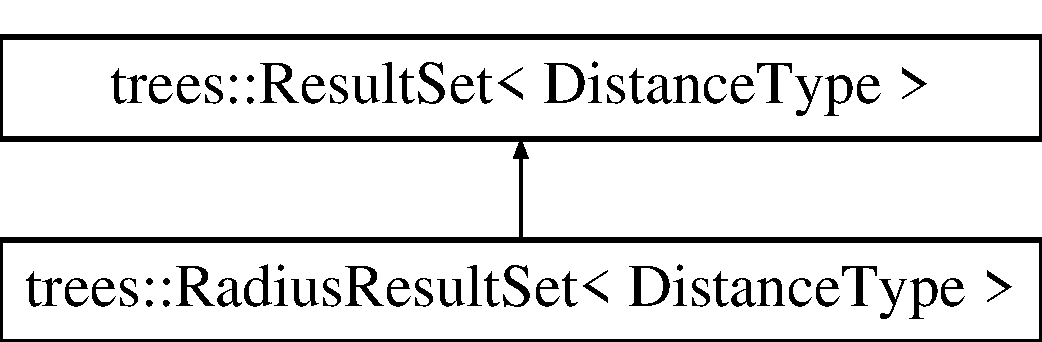
\includegraphics[height=2.000000cm]{classtrees_1_1_radius_result_set}
\end{center}
\end{figure}
\subsection*{Public Types}
\begin{DoxyCompactItemize}
\item 
\mbox{\Hypertarget{classtrees_1_1_radius_result_set_a553d1b7b948e3647afce9e168b0cf5a4}\label{classtrees_1_1_radius_result_set_a553d1b7b948e3647afce9e168b0cf5a4}} 
typedef \hyperlink{structtrees_1_1_distance_index}{Distance\+Index}$<$ Distance\+Type $>$ {\bfseries Dist\+Index}
\end{DoxyCompactItemize}
\subsection*{Public Member Functions}
\begin{DoxyCompactItemize}
\item 
\mbox{\Hypertarget{classtrees_1_1_radius_result_set_a0db3556f2cbe54ef66ca8c3f1d753592}\label{classtrees_1_1_radius_result_set_a0db3556f2cbe54ef66ca8c3f1d753592}} 
{\bfseries Radius\+Result\+Set} (Distance\+Type radius\+\_\+)
\item 
void \hyperlink{classtrees_1_1_radius_result_set_a4e41825c25577341937de798be4ab659}{clear} ()
\item 
size\+\_\+t \hyperlink{classtrees_1_1_radius_result_set_a4ac769fcfb64d84d46d0eb233d4681da}{size} () const
\item 
bool \hyperlink{classtrees_1_1_radius_result_set_a25ad92a894e2b78556bb3c781b2cc173}{full} () const
\item 
void \hyperlink{classtrees_1_1_radius_result_set_a65652623444c8beb35a1d27a86117b2a}{add\+Point} (Distance\+Type dist, size\+\_\+t index)
\item 
void \hyperlink{classtrees_1_1_radius_result_set_aad21bfbfd64e9e1a4fb5d5f80daf84b8}{copy} (size\+\_\+t $\ast$indices, Distance\+Type $\ast$dists, size\+\_\+t num\+\_\+elements, bool sorted=true)
\item 
\mbox{\Hypertarget{classtrees_1_1_radius_result_set_a676e9763ca183b970e5cda2f39ffcbc5}\label{classtrees_1_1_radius_result_set_a676e9763ca183b970e5cda2f39ffcbc5}} 
Distance\+Type {\bfseries worst\+Dist} () const
\end{DoxyCompactItemize}
\subsection*{Additional Inherited Members}


\subsection{Detailed Description}
\subsubsection*{template$<$typename Distance\+Type$>$\newline
class trees\+::\+Radius\+Result\+Set$<$ Distance\+Type $>$}

Unbounded radius result set. It will hold as many elements as are added to it. 

\subsection{Member Function Documentation}
\mbox{\Hypertarget{classtrees_1_1_radius_result_set_a65652623444c8beb35a1d27a86117b2a}\label{classtrees_1_1_radius_result_set_a65652623444c8beb35a1d27a86117b2a}} 
\index{trees\+::\+Radius\+Result\+Set@{trees\+::\+Radius\+Result\+Set}!add\+Point@{add\+Point}}
\index{add\+Point@{add\+Point}!trees\+::\+Radius\+Result\+Set@{trees\+::\+Radius\+Result\+Set}}
\subsubsection{\texorpdfstring{add\+Point()}{addPoint()}}
{\footnotesize\ttfamily template$<$typename Distance\+Type $>$ \\
void \hyperlink{classtrees_1_1_radius_result_set}{trees\+::\+Radius\+Result\+Set}$<$ Distance\+Type $>$\+::add\+Point (\begin{DoxyParamCaption}\item[{Distance\+Type}]{dist,  }\item[{size\+\_\+t}]{index }\end{DoxyParamCaption})\hspace{0.3cm}{\ttfamily [inline]}, {\ttfamily [virtual]}}

Add another point to result set 
\begin{DoxyParams}{Parameters}
{\em dist} & distance to point \\
\hline
{\em index} & index of point Pre-\/conditions\+: capacity\+\_\+$>$0 \\
\hline
\end{DoxyParams}


Implements \hyperlink{classtrees_1_1_result_set}{trees\+::\+Result\+Set$<$ Distance\+Type $>$}.

\mbox{\Hypertarget{classtrees_1_1_radius_result_set_a4e41825c25577341937de798be4ab659}\label{classtrees_1_1_radius_result_set_a4e41825c25577341937de798be4ab659}} 
\index{trees\+::\+Radius\+Result\+Set@{trees\+::\+Radius\+Result\+Set}!clear@{clear}}
\index{clear@{clear}!trees\+::\+Radius\+Result\+Set@{trees\+::\+Radius\+Result\+Set}}
\subsubsection{\texorpdfstring{clear()}{clear()}}
{\footnotesize\ttfamily template$<$typename Distance\+Type $>$ \\
void \hyperlink{classtrees_1_1_radius_result_set}{trees\+::\+Radius\+Result\+Set}$<$ Distance\+Type $>$\+::clear (\begin{DoxyParamCaption}{ }\end{DoxyParamCaption})\hspace{0.3cm}{\ttfamily [inline]}}

Clears the result set \mbox{\Hypertarget{classtrees_1_1_radius_result_set_aad21bfbfd64e9e1a4fb5d5f80daf84b8}\label{classtrees_1_1_radius_result_set_aad21bfbfd64e9e1a4fb5d5f80daf84b8}} 
\index{trees\+::\+Radius\+Result\+Set@{trees\+::\+Radius\+Result\+Set}!copy@{copy}}
\index{copy@{copy}!trees\+::\+Radius\+Result\+Set@{trees\+::\+Radius\+Result\+Set}}
\subsubsection{\texorpdfstring{copy()}{copy()}}
{\footnotesize\ttfamily template$<$typename Distance\+Type $>$ \\
void \hyperlink{classtrees_1_1_radius_result_set}{trees\+::\+Radius\+Result\+Set}$<$ Distance\+Type $>$\+::copy (\begin{DoxyParamCaption}\item[{size\+\_\+t $\ast$}]{indices,  }\item[{Distance\+Type $\ast$}]{dists,  }\item[{size\+\_\+t}]{num\+\_\+elements,  }\item[{bool}]{sorted = {\ttfamily true} }\end{DoxyParamCaption})\hspace{0.3cm}{\ttfamily [inline]}}

Copy indices and distances to output buffers 
\begin{DoxyParams}{Parameters}
{\em indices} & \\
\hline
{\em dists} & \\
\hline
{\em num\+\_\+elements} & Number of elements to copy \\
\hline
{\em sorted} & Indicates if results should be sorted \\
\hline
\end{DoxyParams}
\mbox{\Hypertarget{classtrees_1_1_radius_result_set_a25ad92a894e2b78556bb3c781b2cc173}\label{classtrees_1_1_radius_result_set_a25ad92a894e2b78556bb3c781b2cc173}} 
\index{trees\+::\+Radius\+Result\+Set@{trees\+::\+Radius\+Result\+Set}!full@{full}}
\index{full@{full}!trees\+::\+Radius\+Result\+Set@{trees\+::\+Radius\+Result\+Set}}
\subsubsection{\texorpdfstring{full()}{full()}}
{\footnotesize\ttfamily template$<$typename Distance\+Type $>$ \\
bool \hyperlink{classtrees_1_1_radius_result_set}{trees\+::\+Radius\+Result\+Set}$<$ Distance\+Type $>$\+::full (\begin{DoxyParamCaption}{ }\end{DoxyParamCaption}) const\hspace{0.3cm}{\ttfamily [inline]}, {\ttfamily [virtual]}}

Radius search result set always reports full \begin{DoxyReturn}{Returns}

\end{DoxyReturn}


Implements \hyperlink{classtrees_1_1_result_set}{trees\+::\+Result\+Set$<$ Distance\+Type $>$}.

\mbox{\Hypertarget{classtrees_1_1_radius_result_set_a4ac769fcfb64d84d46d0eb233d4681da}\label{classtrees_1_1_radius_result_set_a4ac769fcfb64d84d46d0eb233d4681da}} 
\index{trees\+::\+Radius\+Result\+Set@{trees\+::\+Radius\+Result\+Set}!size@{size}}
\index{size@{size}!trees\+::\+Radius\+Result\+Set@{trees\+::\+Radius\+Result\+Set}}
\subsubsection{\texorpdfstring{size()}{size()}}
{\footnotesize\ttfamily template$<$typename Distance\+Type $>$ \\
size\+\_\+t \hyperlink{classtrees_1_1_radius_result_set}{trees\+::\+Radius\+Result\+Set}$<$ Distance\+Type $>$\+::size (\begin{DoxyParamCaption}{ }\end{DoxyParamCaption}) const\hspace{0.3cm}{\ttfamily [inline]}}

\begin{DoxyReturn}{Returns}
Number of elements in the result set 
\end{DoxyReturn}


The documentation for this class was generated from the following file\+:\begin{DoxyCompactItemize}
\item 
util/result\+\_\+set.\+h\end{DoxyCompactItemize}

\hypertarget{classtrees_1_1_radius_unique_result_set}{}\section{trees\+:\+:Radius\+Unique\+Result\+Set$<$ Distance\+Type $>$ Class Template Reference}
\label{classtrees_1_1_radius_unique_result_set}\index{trees\+::\+Radius\+Unique\+Result\+Set$<$ Distance\+Type $>$@{trees\+::\+Radius\+Unique\+Result\+Set$<$ Distance\+Type $>$}}


{\ttfamily \#include $<$result\+\_\+set.\+h$>$}

Inheritance diagram for trees\+:\+:Radius\+Unique\+Result\+Set$<$ Distance\+Type $>$\+:\begin{figure}[H]
\begin{center}
\leavevmode
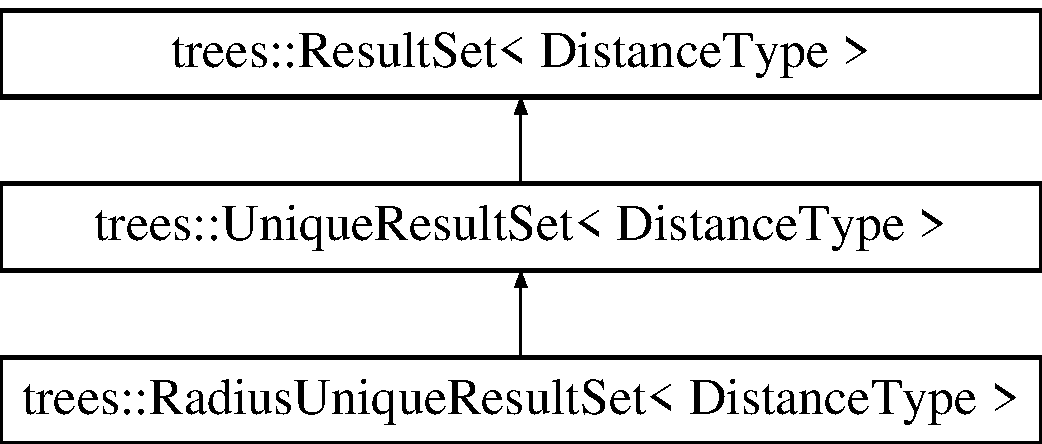
\includegraphics[height=3.000000cm]{classtrees_1_1_radius_unique_result_set}
\end{center}
\end{figure}
\subsection*{Public Member Functions}
\begin{DoxyCompactItemize}
\item 
\hyperlink{classtrees_1_1_radius_unique_result_set_a257fdf0c924ab9077613c2dc1a3b18ea}{Radius\+Unique\+Result\+Set} (Distance\+Type radius)
\item 
void \hyperlink{classtrees_1_1_radius_unique_result_set_ad354a9cee46aa287bb6f9d6bfde50e94}{add\+Point} (Distance\+Type dist, size\+\_\+t index)
\item 
void \hyperlink{classtrees_1_1_radius_unique_result_set_a1931c3241af134573cb3021f735c469c}{clear} ()
\item 
bool \hyperlink{classtrees_1_1_radius_unique_result_set_a0a402d8fb16cfaa233d43bdcb5b3ab97}{full} () const
\item 
Distance\+Type \hyperlink{classtrees_1_1_radius_unique_result_set_af0f7ec26a6515cb085df64a43afe433c}{worst\+Dist} () const
\end{DoxyCompactItemize}
\subsection*{Additional Inherited Members}


\subsection{Detailed Description}
\subsubsection*{template$<$typename Distance\+Type$>$\newline
class trees\+::\+Radius\+Unique\+Result\+Set$<$ Distance\+Type $>$}

Class that holds the radius nearest neighbors It is more accurate than Radius\+Result as it is not limited in the number of neighbors 

\subsection{Constructor \& Destructor Documentation}
\mbox{\Hypertarget{classtrees_1_1_radius_unique_result_set_a257fdf0c924ab9077613c2dc1a3b18ea}\label{classtrees_1_1_radius_unique_result_set_a257fdf0c924ab9077613c2dc1a3b18ea}} 
\index{trees\+::\+Radius\+Unique\+Result\+Set@{trees\+::\+Radius\+Unique\+Result\+Set}!Radius\+Unique\+Result\+Set@{Radius\+Unique\+Result\+Set}}
\index{Radius\+Unique\+Result\+Set@{Radius\+Unique\+Result\+Set}!trees\+::\+Radius\+Unique\+Result\+Set@{trees\+::\+Radius\+Unique\+Result\+Set}}
\subsubsection{\texorpdfstring{Radius\+Unique\+Result\+Set()}{RadiusUniqueResultSet()}}
{\footnotesize\ttfamily template$<$typename Distance\+Type $>$ \\
\hyperlink{classtrees_1_1_radius_unique_result_set}{trees\+::\+Radius\+Unique\+Result\+Set}$<$ Distance\+Type $>$\+::\hyperlink{classtrees_1_1_radius_unique_result_set}{Radius\+Unique\+Result\+Set} (\begin{DoxyParamCaption}\item[{Distance\+Type}]{radius }\end{DoxyParamCaption})\hspace{0.3cm}{\ttfamily [inline]}}

Constructor 
\begin{DoxyParams}{Parameters}
{\em capacity} & the number of neighbors to store at max \\
\hline
\end{DoxyParams}


\subsection{Member Function Documentation}
\mbox{\Hypertarget{classtrees_1_1_radius_unique_result_set_ad354a9cee46aa287bb6f9d6bfde50e94}\label{classtrees_1_1_radius_unique_result_set_ad354a9cee46aa287bb6f9d6bfde50e94}} 
\index{trees\+::\+Radius\+Unique\+Result\+Set@{trees\+::\+Radius\+Unique\+Result\+Set}!add\+Point@{add\+Point}}
\index{add\+Point@{add\+Point}!trees\+::\+Radius\+Unique\+Result\+Set@{trees\+::\+Radius\+Unique\+Result\+Set}}
\subsubsection{\texorpdfstring{add\+Point()}{addPoint()}}
{\footnotesize\ttfamily template$<$typename Distance\+Type $>$ \\
void \hyperlink{classtrees_1_1_radius_unique_result_set}{trees\+::\+Radius\+Unique\+Result\+Set}$<$ Distance\+Type $>$\+::add\+Point (\begin{DoxyParamCaption}\item[{Distance\+Type}]{dist,  }\item[{size\+\_\+t}]{index }\end{DoxyParamCaption})\hspace{0.3cm}{\ttfamily [inline]}, {\ttfamily [virtual]}}

Add a possible candidate to the best neighbors 
\begin{DoxyParams}{Parameters}
{\em dist} & distance for that neighbor \\
\hline
{\em index} & index of that neighbor \\
\hline
\end{DoxyParams}


Implements \hyperlink{classtrees_1_1_result_set}{trees\+::\+Result\+Set$<$ Distance\+Type $>$}.

\mbox{\Hypertarget{classtrees_1_1_radius_unique_result_set_a1931c3241af134573cb3021f735c469c}\label{classtrees_1_1_radius_unique_result_set_a1931c3241af134573cb3021f735c469c}} 
\index{trees\+::\+Radius\+Unique\+Result\+Set@{trees\+::\+Radius\+Unique\+Result\+Set}!clear@{clear}}
\index{clear@{clear}!trees\+::\+Radius\+Unique\+Result\+Set@{trees\+::\+Radius\+Unique\+Result\+Set}}
\subsubsection{\texorpdfstring{clear()}{clear()}}
{\footnotesize\ttfamily template$<$typename Distance\+Type $>$ \\
void \hyperlink{classtrees_1_1_radius_unique_result_set}{trees\+::\+Radius\+Unique\+Result\+Set}$<$ Distance\+Type $>$\+::clear (\begin{DoxyParamCaption}{ }\end{DoxyParamCaption})\hspace{0.3cm}{\ttfamily [inline]}}

Remove all elements in the set \mbox{\Hypertarget{classtrees_1_1_radius_unique_result_set_a0a402d8fb16cfaa233d43bdcb5b3ab97}\label{classtrees_1_1_radius_unique_result_set_a0a402d8fb16cfaa233d43bdcb5b3ab97}} 
\index{trees\+::\+Radius\+Unique\+Result\+Set@{trees\+::\+Radius\+Unique\+Result\+Set}!full@{full}}
\index{full@{full}!trees\+::\+Radius\+Unique\+Result\+Set@{trees\+::\+Radius\+Unique\+Result\+Set}}
\subsubsection{\texorpdfstring{full()}{full()}}
{\footnotesize\ttfamily template$<$typename Distance\+Type $>$ \\
bool \hyperlink{classtrees_1_1_radius_unique_result_set}{trees\+::\+Radius\+Unique\+Result\+Set}$<$ Distance\+Type $>$\+::full (\begin{DoxyParamCaption}{ }\end{DoxyParamCaption}) const\hspace{0.3cm}{\ttfamily [inline]}, {\ttfamily [virtual]}}

Check the status of the set \begin{DoxyReturn}{Returns}
alwys false 
\end{DoxyReturn}


Reimplemented from \hyperlink{classtrees_1_1_unique_result_set_a6c10f8635c22eaecaa7e6fda3afea132}{trees\+::\+Unique\+Result\+Set$<$ Distance\+Type $>$}.

\mbox{\Hypertarget{classtrees_1_1_radius_unique_result_set_af0f7ec26a6515cb085df64a43afe433c}\label{classtrees_1_1_radius_unique_result_set_af0f7ec26a6515cb085df64a43afe433c}} 
\index{trees\+::\+Radius\+Unique\+Result\+Set@{trees\+::\+Radius\+Unique\+Result\+Set}!worst\+Dist@{worst\+Dist}}
\index{worst\+Dist@{worst\+Dist}!trees\+::\+Radius\+Unique\+Result\+Set@{trees\+::\+Radius\+Unique\+Result\+Set}}
\subsubsection{\texorpdfstring{worst\+Dist()}{worstDist()}}
{\footnotesize\ttfamily template$<$typename Distance\+Type $>$ \\
Distance\+Type \hyperlink{classtrees_1_1_radius_unique_result_set}{trees\+::\+Radius\+Unique\+Result\+Set}$<$ Distance\+Type $>$\+::worst\+Dist (\begin{DoxyParamCaption}{ }\end{DoxyParamCaption}) const\hspace{0.3cm}{\ttfamily [inline]}, {\ttfamily [virtual]}}

The distance of the furthest neighbor If we don\textquotesingle{}t have enough neighbors, it returns the max possible value \begin{DoxyReturn}{Returns}

\end{DoxyReturn}


Reimplemented from \hyperlink{classtrees_1_1_unique_result_set_a2301eba6dae87959cc50668dd2307d4d}{trees\+::\+Unique\+Result\+Set$<$ Distance\+Type $>$}.



The documentation for this class was generated from the following file\+:\begin{DoxyCompactItemize}
\item 
util/result\+\_\+set.\+h\end{DoxyCompactItemize}

\hypertarget{classtrees_1_1_result_set}{}\section{trees\+:\+:Result\+Set$<$ Distance\+Type $>$ Class Template Reference}
\label{classtrees_1_1_result_set}\index{trees\+::\+Result\+Set$<$ Distance\+Type $>$@{trees\+::\+Result\+Set$<$ Distance\+Type $>$}}
Inheritance diagram for trees\+:\+:Result\+Set$<$ Distance\+Type $>$\+:\begin{figure}[H]
\begin{center}
\leavevmode
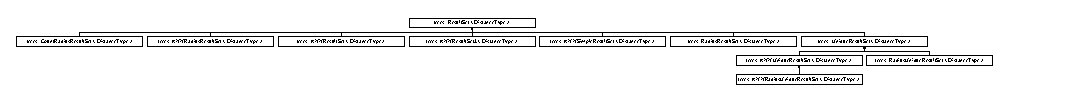
\includegraphics[height=0.906149cm]{classtrees_1_1_result_set}
\end{center}
\end{figure}
\subsection*{Public Member Functions}
\begin{DoxyCompactItemize}
\item 
\mbox{\Hypertarget{classtrees_1_1_result_set_afe172e3581433bcc46fecdbb156cde8b}\label{classtrees_1_1_result_set_afe172e3581433bcc46fecdbb156cde8b}} 
{\bfseries Result\+Set} (size\+\_\+t capacity\+\_\+)
\item 
\mbox{\Hypertarget{classtrees_1_1_result_set_ac35ee245b34f1f37fefbe994e85f5de5}\label{classtrees_1_1_result_set_ac35ee245b34f1f37fefbe994e85f5de5}} 
virtual bool {\bfseries full} () const =0
\item 
\mbox{\Hypertarget{classtrees_1_1_result_set_a168f89986f238cd4e43e8a5e80bec025}\label{classtrees_1_1_result_set_a168f89986f238cd4e43e8a5e80bec025}} 
virtual void {\bfseries add\+Point} (Distance\+Type dist, size\+\_\+t index)=0
\item 
\mbox{\Hypertarget{classtrees_1_1_result_set_a7e060d29f148a5d54cfb3e8ac63f8c18}\label{classtrees_1_1_result_set_a7e060d29f148a5d54cfb3e8ac63f8c18}} 
virtual Distance\+Type {\bfseries worst\+Dist} () const =0
\end{DoxyCompactItemize}
\subsection*{Public Attributes}
\begin{DoxyCompactItemize}
\item 
\mbox{\Hypertarget{classtrees_1_1_result_set_ab38709e3e9911c7ff7598ab368dfdba1}\label{classtrees_1_1_result_set_ab38709e3e9911c7ff7598ab368dfdba1}} 
size\+\_\+t {\bfseries capacity\+\_\+}
\end{DoxyCompactItemize}


The documentation for this class was generated from the following file\+:\begin{DoxyCompactItemize}
\item 
utils/result\+\_\+set.\+h\end{DoxyCompactItemize}

\hypertarget{structtrees_1_1anyimpl_1_1small__any__policy}{}\section{trees\+:\+:anyimpl\+:\+:small\+\_\+any\+\_\+policy$<$ T $>$ Struct Template Reference}
\label{structtrees_1_1anyimpl_1_1small__any__policy}\index{trees\+::anyimpl\+::small\+\_\+any\+\_\+policy$<$ T $>$@{trees\+::anyimpl\+::small\+\_\+any\+\_\+policy$<$ T $>$}}
Inheritance diagram for trees\+:\+:anyimpl\+:\+:small\+\_\+any\+\_\+policy$<$ T $>$\+:\begin{figure}[H]
\begin{center}
\leavevmode
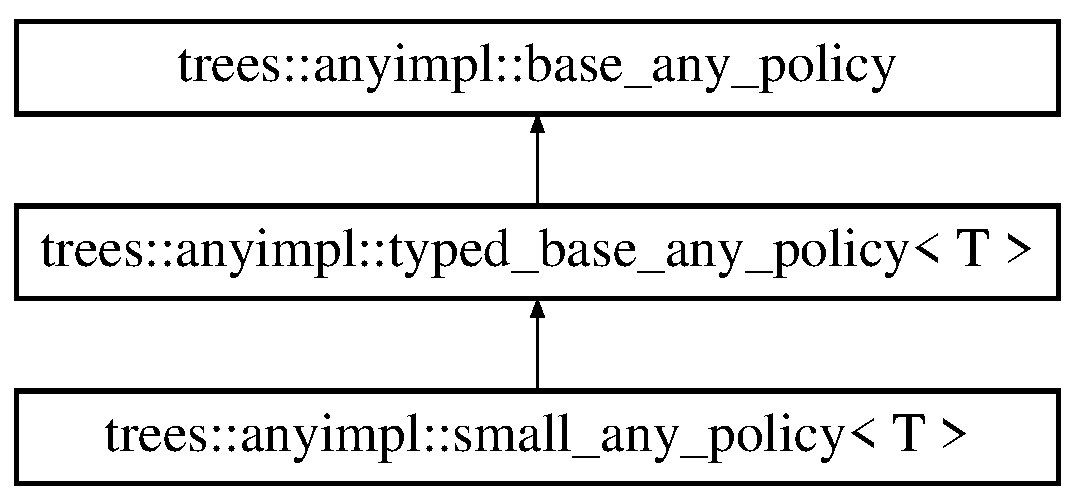
\includegraphics[height=3.000000cm]{structtrees_1_1anyimpl_1_1small__any__policy}
\end{center}
\end{figure}
\subsection*{Public Member Functions}
\begin{DoxyCompactItemize}
\item 
\mbox{\Hypertarget{structtrees_1_1anyimpl_1_1small__any__policy_a88ca9c077624b4396d47259e7ebc4e2a}\label{structtrees_1_1anyimpl_1_1small__any__policy_a88ca9c077624b4396d47259e7ebc4e2a}} 
virtual void {\bfseries static\+\_\+delete} (void $\ast$$\ast$)
\item 
\mbox{\Hypertarget{structtrees_1_1anyimpl_1_1small__any__policy_a44215871b9ab01baf4be240e87045f26}\label{structtrees_1_1anyimpl_1_1small__any__policy_a44215871b9ab01baf4be240e87045f26}} 
virtual void {\bfseries copy\+\_\+from\+\_\+value} (void const $\ast$src, void $\ast$$\ast$dest)
\item 
\mbox{\Hypertarget{structtrees_1_1anyimpl_1_1small__any__policy_ac6333d36ba39556ca71c71e40832adfb}\label{structtrees_1_1anyimpl_1_1small__any__policy_ac6333d36ba39556ca71c71e40832adfb}} 
virtual void {\bfseries clone} (void $\ast$const $\ast$src, void $\ast$$\ast$dest)
\item 
\mbox{\Hypertarget{structtrees_1_1anyimpl_1_1small__any__policy_acefd3b911628bab13d2c678a59025fba}\label{structtrees_1_1anyimpl_1_1small__any__policy_acefd3b911628bab13d2c678a59025fba}} 
virtual void {\bfseries move} (void $\ast$const $\ast$src, void $\ast$$\ast$dest)
\item 
\mbox{\Hypertarget{structtrees_1_1anyimpl_1_1small__any__policy_ae6cb7097f85171cef9c31088028e0793}\label{structtrees_1_1anyimpl_1_1small__any__policy_ae6cb7097f85171cef9c31088028e0793}} 
virtual void $\ast$ {\bfseries get\+\_\+value} (void $\ast$$\ast$src)
\item 
\mbox{\Hypertarget{structtrees_1_1anyimpl_1_1small__any__policy_a9c11969bd2dcc3337f47f1a061c4bcb5}\label{structtrees_1_1anyimpl_1_1small__any__policy_a9c11969bd2dcc3337f47f1a061c4bcb5}} 
virtual const void $\ast$ {\bfseries get\+\_\+value} (void $\ast$const $\ast$src)
\item 
\mbox{\Hypertarget{structtrees_1_1anyimpl_1_1small__any__policy_a2046f30eeae5653ae3d5fbd1d53e0ced}\label{structtrees_1_1anyimpl_1_1small__any__policy_a2046f30eeae5653ae3d5fbd1d53e0ced}} 
virtual void {\bfseries print} (std\+::ostream \&out, void $\ast$const $\ast$src)
\end{DoxyCompactItemize}


The documentation for this struct was generated from the following file\+:\begin{DoxyCompactItemize}
\item 
util/any.\+h\end{DoxyCompactItemize}

\hypertarget{classtrees_1_1_threadpool}{}\section{trees\+:\+:Threadpool Class Reference}
\label{classtrees_1_1_threadpool}\index{trees\+::\+Threadpool@{trees\+::\+Threadpool}}
\subsection*{Public Member Functions}
\begin{DoxyCompactItemize}
\item 
\hyperlink{classtrees_1_1_threadpool_a2ddeee4f43093bc52ff011213def07e4}{Threadpool} (std\+::size\+\_\+t pool\+\_\+)
\item 
\hyperlink{classtrees_1_1_threadpool_afb783a8a8b881f2f0be9cae58550d345}{$\sim$\+Threadpool} ()
\item 
void \hyperlink{classtrees_1_1_threadpool_a3d6488b730cc53472239f9c74e384d64}{shutdown} ()
\item 
{\footnotesize template$<$typename Task $>$ }\\bool \hyperlink{classtrees_1_1_threadpool_a5aa569f51cc6095e8017500c7e6b074d}{run\+Task} (Task task\+\_\+)
\item 
bool \hyperlink{classtrees_1_1_threadpool_a5675fede770bf61c78cdd2d0250acc93}{wait\+Tasks} ()
\end{DoxyCompactItemize}


\subsection{Constructor \& Destructor Documentation}
\mbox{\Hypertarget{classtrees_1_1_threadpool_a2ddeee4f43093bc52ff011213def07e4}\label{classtrees_1_1_threadpool_a2ddeee4f43093bc52ff011213def07e4}} 
\index{trees\+::\+Threadpool@{trees\+::\+Threadpool}!Threadpool@{Threadpool}}
\index{Threadpool@{Threadpool}!trees\+::\+Threadpool@{trees\+::\+Threadpool}}
\subsubsection{\texorpdfstring{Threadpool()}{Threadpool()}}
{\footnotesize\ttfamily trees\+::\+Threadpool\+::\+Threadpool (\begin{DoxyParamCaption}\item[{std\+::size\+\_\+t}]{pool\+\_\+ }\end{DoxyParamCaption})\hspace{0.3cm}{\ttfamily [inline]}}

Constructor


\begin{DoxyParams}[1]{Parameters}
\mbox{\tt in}  & {\em pool\+\_\+} & Number of active threads \\
\hline
\end{DoxyParams}
\mbox{\Hypertarget{classtrees_1_1_threadpool_afb783a8a8b881f2f0be9cae58550d345}\label{classtrees_1_1_threadpool_afb783a8a8b881f2f0be9cae58550d345}} 
\index{trees\+::\+Threadpool@{trees\+::\+Threadpool}!````~Threadpool@{$\sim$\+Threadpool}}
\index{````~Threadpool@{$\sim$\+Threadpool}!trees\+::\+Threadpool@{trees\+::\+Threadpool}}
\subsubsection{\texorpdfstring{$\sim$\+Threadpool()}{~Threadpool()}}
{\footnotesize\ttfamily trees\+::\+Threadpool\+::$\sim$\+Threadpool (\begin{DoxyParamCaption}{ }\end{DoxyParamCaption})\hspace{0.3cm}{\ttfamily [inline]}}

Destructor 

\subsection{Member Function Documentation}
\mbox{\Hypertarget{classtrees_1_1_threadpool_a5aa569f51cc6095e8017500c7e6b074d}\label{classtrees_1_1_threadpool_a5aa569f51cc6095e8017500c7e6b074d}} 
\index{trees\+::\+Threadpool@{trees\+::\+Threadpool}!run\+Task@{run\+Task}}
\index{run\+Task@{run\+Task}!trees\+::\+Threadpool@{trees\+::\+Threadpool}}
\subsubsection{\texorpdfstring{run\+Task()}{runTask()}}
{\footnotesize\ttfamily template$<$typename Task $>$ \\
bool trees\+::\+Threadpool\+::run\+Task (\begin{DoxyParamCaption}\item[{Task}]{task\+\_\+ }\end{DoxyParamCaption})\hspace{0.3cm}{\ttfamily [inline]}}

Start a thread with a specific task


\begin{DoxyParams}[1]{Parameters}
\mbox{\tt in}  & {\em task\+\_\+} & Function which will be invoked \\
\hline
\end{DoxyParams}
\begin{DoxyReturn}{Returns}
True if the function could be invoked 
\end{DoxyReturn}
\mbox{\Hypertarget{classtrees_1_1_threadpool_a3d6488b730cc53472239f9c74e384d64}\label{classtrees_1_1_threadpool_a3d6488b730cc53472239f9c74e384d64}} 
\index{trees\+::\+Threadpool@{trees\+::\+Threadpool}!shutdown@{shutdown}}
\index{shutdown@{shutdown}!trees\+::\+Threadpool@{trees\+::\+Threadpool}}
\subsubsection{\texorpdfstring{shutdown()}{shutdown()}}
{\footnotesize\ttfamily void trees\+::\+Threadpool\+::shutdown (\begin{DoxyParamCaption}{ }\end{DoxyParamCaption})\hspace{0.3cm}{\ttfamily [inline]}}

Terminates io\+\_\+service and threads \mbox{\Hypertarget{classtrees_1_1_threadpool_a5675fede770bf61c78cdd2d0250acc93}\label{classtrees_1_1_threadpool_a5675fede770bf61c78cdd2d0250acc93}} 
\index{trees\+::\+Threadpool@{trees\+::\+Threadpool}!wait\+Tasks@{wait\+Tasks}}
\index{wait\+Tasks@{wait\+Tasks}!trees\+::\+Threadpool@{trees\+::\+Threadpool}}
\subsubsection{\texorpdfstring{wait\+Tasks()}{waitTasks()}}
{\footnotesize\ttfamily bool trees\+::\+Threadpool\+::wait\+Tasks (\begin{DoxyParamCaption}{ }\end{DoxyParamCaption})\hspace{0.3cm}{\ttfamily [inline]}}

Waits until all threads has been finished

\begin{DoxyReturn}{Returns}
Return true if all tasks are completed 
\end{DoxyReturn}


The documentation for this class was generated from the following file\+:\begin{DoxyCompactItemize}
\item 
util/threadpool.\+h\end{DoxyCompactItemize}

\hypertarget{structtrees_1_1_tree_params}{}\section{trees\+:\+:Tree\+Params Struct Reference}
\label{structtrees_1_1_tree_params}\index{trees\+::\+Tree\+Params@{trees\+::\+Tree\+Params}}


{\ttfamily \#include $<$params.\+h$>$}

\subsection*{Public Member Functions}
\begin{DoxyCompactItemize}
\item 
\hyperlink{structtrees_1_1_tree_params_a0f5ed74837938da3ff41a8c95a6edfd8}{Tree\+Params} (int cores\+\_\+=1, float eps\+\_\+=std\+::numeric\+\_\+limits$<$ float $>$\+::epsilon())
\end{DoxyCompactItemize}
\subsection*{Public Attributes}
\begin{DoxyCompactItemize}
\item 
int \hyperlink{structtrees_1_1_tree_params_a5ef0f40ea5395de102678757741c65c6}{cores}
\item 
float \hyperlink{structtrees_1_1_tree_params_abeaacd2b7ddb9f7345595f90a3926176}{eps}
\end{DoxyCompactItemize}


\subsection{Detailed Description}
Structure which holds tree parameters 

\subsection{Constructor \& Destructor Documentation}
\mbox{\Hypertarget{structtrees_1_1_tree_params_a0f5ed74837938da3ff41a8c95a6edfd8}\label{structtrees_1_1_tree_params_a0f5ed74837938da3ff41a8c95a6edfd8}} 
\index{trees\+::\+Tree\+Params@{trees\+::\+Tree\+Params}!Tree\+Params@{Tree\+Params}}
\index{Tree\+Params@{Tree\+Params}!trees\+::\+Tree\+Params@{trees\+::\+Tree\+Params}}
\subsubsection{\texorpdfstring{Tree\+Params()}{TreeParams()}}
{\footnotesize\ttfamily trees\+::\+Tree\+Params\+::\+Tree\+Params (\begin{DoxyParamCaption}\item[{int}]{cores\+\_\+ = {\ttfamily 1},  }\item[{float}]{eps\+\_\+ = {\ttfamily std\+:\+:numeric\+\_\+limits$<$float$>$\+:\+:epsilon()} }\end{DoxyParamCaption})\hspace{0.3cm}{\ttfamily [inline]}}

Constructor


\begin{DoxyParams}[1]{Parameters}
\mbox{\tt in}  & {\em cores\+\_\+} & Number of cores \\
\hline
\mbox{\tt in}  & {\em eps\+\_\+} & Machine epsilon \\
\hline
\end{DoxyParams}


\subsection{Member Data Documentation}
\mbox{\Hypertarget{structtrees_1_1_tree_params_a5ef0f40ea5395de102678757741c65c6}\label{structtrees_1_1_tree_params_a5ef0f40ea5395de102678757741c65c6}} 
\index{trees\+::\+Tree\+Params@{trees\+::\+Tree\+Params}!cores@{cores}}
\index{cores@{cores}!trees\+::\+Tree\+Params@{trees\+::\+Tree\+Params}}
\subsubsection{\texorpdfstring{cores}{cores}}
{\footnotesize\ttfamily int trees\+::\+Tree\+Params\+::cores}

Number of cores \mbox{\Hypertarget{structtrees_1_1_tree_params_abeaacd2b7ddb9f7345595f90a3926176}\label{structtrees_1_1_tree_params_abeaacd2b7ddb9f7345595f90a3926176}} 
\index{trees\+::\+Tree\+Params@{trees\+::\+Tree\+Params}!eps@{eps}}
\index{eps@{eps}!trees\+::\+Tree\+Params@{trees\+::\+Tree\+Params}}
\subsubsection{\texorpdfstring{eps}{eps}}
{\footnotesize\ttfamily float trees\+::\+Tree\+Params\+::eps}

Machine epsilon 

The documentation for this struct was generated from the following file\+:\begin{DoxyCompactItemize}
\item 
utils/params.\+h\end{DoxyCompactItemize}

\hypertarget{structtrees_1_1anyimpl_1_1typed__base__any__policy}{}\section{trees\+:\+:anyimpl\+:\+:typed\+\_\+base\+\_\+any\+\_\+policy$<$ T $>$ Struct Template Reference}
\label{structtrees_1_1anyimpl_1_1typed__base__any__policy}\index{trees\+::anyimpl\+::typed\+\_\+base\+\_\+any\+\_\+policy$<$ T $>$@{trees\+::anyimpl\+::typed\+\_\+base\+\_\+any\+\_\+policy$<$ T $>$}}
Inheritance diagram for trees\+:\+:anyimpl\+:\+:typed\+\_\+base\+\_\+any\+\_\+policy$<$ T $>$\+:\begin{figure}[H]
\begin{center}
\leavevmode
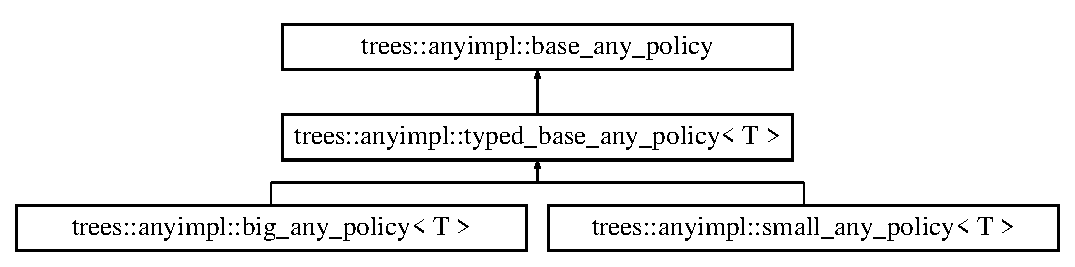
\includegraphics[height=3.000000cm]{structtrees_1_1anyimpl_1_1typed__base__any__policy}
\end{center}
\end{figure}
\subsection*{Public Member Functions}
\begin{DoxyCompactItemize}
\item 
\mbox{\Hypertarget{structtrees_1_1anyimpl_1_1typed__base__any__policy_a8d6c211c812bfa394a34125a09ea286b}\label{structtrees_1_1anyimpl_1_1typed__base__any__policy_a8d6c211c812bfa394a34125a09ea286b}} 
virtual \+::size\+\_\+t {\bfseries get\+\_\+size} ()
\item 
\mbox{\Hypertarget{structtrees_1_1anyimpl_1_1typed__base__any__policy_af9870525db7bb196331083b38552713d}\label{structtrees_1_1anyimpl_1_1typed__base__any__policy_af9870525db7bb196331083b38552713d}} 
virtual const std\+::type\+\_\+info \& {\bfseries type} ()
\end{DoxyCompactItemize}


The documentation for this struct was generated from the following file\+:\begin{DoxyCompactItemize}
\item 
util/any.\+h\end{DoxyCompactItemize}

\hypertarget{classtrees_1_1_unique_result_set}{}\section{trees\+:\+:Unique\+Result\+Set$<$ Distance\+Type $>$ Class Template Reference}
\label{classtrees_1_1_unique_result_set}\index{trees\+::\+Unique\+Result\+Set$<$ Distance\+Type $>$@{trees\+::\+Unique\+Result\+Set$<$ Distance\+Type $>$}}


{\ttfamily \#include $<$result\+\_\+set.\+h$>$}

Inheritance diagram for trees\+:\+:Unique\+Result\+Set$<$ Distance\+Type $>$\+:\begin{figure}[H]
\begin{center}
\leavevmode
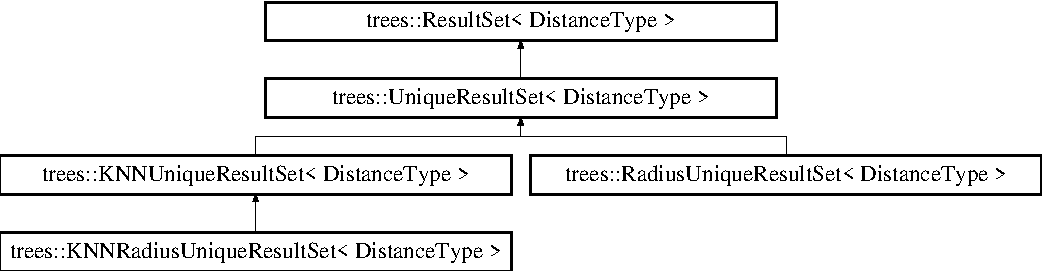
\includegraphics[height=3.624595cm]{classtrees_1_1_unique_result_set}
\end{center}
\end{figure}
\subsection*{Classes}
\begin{DoxyCompactItemize}
\item 
struct \hyperlink{structtrees_1_1_unique_result_set_1_1_dist_index}{Dist\+Index}
\end{DoxyCompactItemize}
\subsection*{Public Member Functions}
\begin{DoxyCompactItemize}
\item 
\hyperlink{classtrees_1_1_unique_result_set_ad1f538e2dcaa431612d537efefc6699e}{Unique\+Result\+Set} ()
\item 
bool \hyperlink{classtrees_1_1_unique_result_set_a6c10f8635c22eaecaa7e6fda3afea132}{full} () const
\item 
void \hyperlink{classtrees_1_1_unique_result_set_a81ab4a644430e524c37a1024628c6b02}{copy} (size\+\_\+t $\ast$indices, Distance\+Type $\ast$dist, int n\+\_\+neighbors, bool sorted=true)
\item 
size\+\_\+t \hyperlink{classtrees_1_1_unique_result_set_a3b0df0041064e4e255e8cc22d142eab8}{size} () const
\item 
Distance\+Type \hyperlink{classtrees_1_1_unique_result_set_a2301eba6dae87959cc50668dd2307d4d}{worst\+Dist} () const
\end{DoxyCompactItemize}
\subsection*{Protected Attributes}
\begin{DoxyCompactItemize}
\item 
bool \hyperlink{classtrees_1_1_unique_result_set_a4d9baa438af8d132f30676f25c5900b4}{is\+\_\+full\+\_\+}
\item 
Distance\+Type \hyperlink{classtrees_1_1_unique_result_set_acdfe562ad6f99ae5f68b7e8af3d68171}{worst\+\_\+distance\+\_\+}
\item 
std\+::set$<$ \hyperlink{structtrees_1_1_unique_result_set_1_1_dist_index}{Dist\+Index} $>$ \hyperlink{classtrees_1_1_unique_result_set_a3a3dd371f4861f0addcfabe8c68ec11c}{dist\+\_\+indices\+\_\+}
\end{DoxyCompactItemize}
\subsection*{Additional Inherited Members}


\subsection{Detailed Description}
\subsubsection*{template$<$typename Distance\+Type$>$\newline
class trees\+::\+Unique\+Result\+Set$<$ Distance\+Type $>$}

Class that holds the k NN neighbors 

\subsection{Constructor \& Destructor Documentation}
\mbox{\Hypertarget{classtrees_1_1_unique_result_set_ad1f538e2dcaa431612d537efefc6699e}\label{classtrees_1_1_unique_result_set_ad1f538e2dcaa431612d537efefc6699e}} 
\index{trees\+::\+Unique\+Result\+Set@{trees\+::\+Unique\+Result\+Set}!Unique\+Result\+Set@{Unique\+Result\+Set}}
\index{Unique\+Result\+Set@{Unique\+Result\+Set}!trees\+::\+Unique\+Result\+Set@{trees\+::\+Unique\+Result\+Set}}
\subsubsection{\texorpdfstring{Unique\+Result\+Set()}{UniqueResultSet()}}
{\footnotesize\ttfamily template$<$typename Distance\+Type $>$ \\
\hyperlink{classtrees_1_1_unique_result_set}{trees\+::\+Unique\+Result\+Set}$<$ Distance\+Type $>$\+::\hyperlink{classtrees_1_1_unique_result_set}{Unique\+Result\+Set} (\begin{DoxyParamCaption}{ }\end{DoxyParamCaption})\hspace{0.3cm}{\ttfamily [inline]}}

Default cosntructor 

\subsection{Member Function Documentation}
\mbox{\Hypertarget{classtrees_1_1_unique_result_set_a81ab4a644430e524c37a1024628c6b02}\label{classtrees_1_1_unique_result_set_a81ab4a644430e524c37a1024628c6b02}} 
\index{trees\+::\+Unique\+Result\+Set@{trees\+::\+Unique\+Result\+Set}!copy@{copy}}
\index{copy@{copy}!trees\+::\+Unique\+Result\+Set@{trees\+::\+Unique\+Result\+Set}}
\subsubsection{\texorpdfstring{copy()}{copy()}}
{\footnotesize\ttfamily template$<$typename Distance\+Type $>$ \\
void \hyperlink{classtrees_1_1_unique_result_set}{trees\+::\+Unique\+Result\+Set}$<$ Distance\+Type $>$\+::copy (\begin{DoxyParamCaption}\item[{size\+\_\+t $\ast$}]{indices,  }\item[{Distance\+Type $\ast$}]{dist,  }\item[{int}]{n\+\_\+neighbors,  }\item[{bool}]{sorted = {\ttfamily true} }\end{DoxyParamCaption})\hspace{0.3cm}{\ttfamily [inline]}}

Copy the set to two C arrays 
\begin{DoxyParams}{Parameters}
{\em indices} & pointer to a C array of indices \\
\hline
{\em dist} & pointer to a C array of distances \\
\hline
{\em n\+\_\+neighbors} & the number of neighbors to copy \\
\hline
\end{DoxyParams}
\mbox{\Hypertarget{classtrees_1_1_unique_result_set_a6c10f8635c22eaecaa7e6fda3afea132}\label{classtrees_1_1_unique_result_set_a6c10f8635c22eaecaa7e6fda3afea132}} 
\index{trees\+::\+Unique\+Result\+Set@{trees\+::\+Unique\+Result\+Set}!full@{full}}
\index{full@{full}!trees\+::\+Unique\+Result\+Set@{trees\+::\+Unique\+Result\+Set}}
\subsubsection{\texorpdfstring{full()}{full()}}
{\footnotesize\ttfamily template$<$typename Distance\+Type $>$ \\
bool \hyperlink{classtrees_1_1_unique_result_set}{trees\+::\+Unique\+Result\+Set}$<$ Distance\+Type $>$\+::full (\begin{DoxyParamCaption}{ }\end{DoxyParamCaption}) const\hspace{0.3cm}{\ttfamily [inline]}, {\ttfamily [virtual]}}

Check the status of the set \begin{DoxyReturn}{Returns}
true if we have k NN 
\end{DoxyReturn}


Implements \hyperlink{classtrees_1_1_result_set}{trees\+::\+Result\+Set$<$ Distance\+Type $>$}.



Reimplemented in \hyperlink{classtrees_1_1_radius_unique_result_set_a0a402d8fb16cfaa233d43bdcb5b3ab97}{trees\+::\+Radius\+Unique\+Result\+Set$<$ Distance\+Type $>$}.

\mbox{\Hypertarget{classtrees_1_1_unique_result_set_a3b0df0041064e4e255e8cc22d142eab8}\label{classtrees_1_1_unique_result_set_a3b0df0041064e4e255e8cc22d142eab8}} 
\index{trees\+::\+Unique\+Result\+Set@{trees\+::\+Unique\+Result\+Set}!size@{size}}
\index{size@{size}!trees\+::\+Unique\+Result\+Set@{trees\+::\+Unique\+Result\+Set}}
\subsubsection{\texorpdfstring{size()}{size()}}
{\footnotesize\ttfamily template$<$typename Distance\+Type $>$ \\
size\+\_\+t \hyperlink{classtrees_1_1_unique_result_set}{trees\+::\+Unique\+Result\+Set}$<$ Distance\+Type $>$\+::size (\begin{DoxyParamCaption}{ }\end{DoxyParamCaption}) const\hspace{0.3cm}{\ttfamily [inline]}}

The number of neighbors in the set \begin{DoxyReturn}{Returns}

\end{DoxyReturn}
\mbox{\Hypertarget{classtrees_1_1_unique_result_set_a2301eba6dae87959cc50668dd2307d4d}\label{classtrees_1_1_unique_result_set_a2301eba6dae87959cc50668dd2307d4d}} 
\index{trees\+::\+Unique\+Result\+Set@{trees\+::\+Unique\+Result\+Set}!worst\+Dist@{worst\+Dist}}
\index{worst\+Dist@{worst\+Dist}!trees\+::\+Unique\+Result\+Set@{trees\+::\+Unique\+Result\+Set}}
\subsubsection{\texorpdfstring{worst\+Dist()}{worstDist()}}
{\footnotesize\ttfamily template$<$typename Distance\+Type $>$ \\
Distance\+Type \hyperlink{classtrees_1_1_unique_result_set}{trees\+::\+Unique\+Result\+Set}$<$ Distance\+Type $>$\+::worst\+Dist (\begin{DoxyParamCaption}{ }\end{DoxyParamCaption}) const\hspace{0.3cm}{\ttfamily [inline]}, {\ttfamily [virtual]}}

The distance of the furthest neighbor If we don\textquotesingle{}t have enough neighbors, it returns the max possible value \begin{DoxyReturn}{Returns}

\end{DoxyReturn}


Implements \hyperlink{classtrees_1_1_result_set}{trees\+::\+Result\+Set$<$ Distance\+Type $>$}.



Reimplemented in \hyperlink{classtrees_1_1_radius_unique_result_set_af0f7ec26a6515cb085df64a43afe433c}{trees\+::\+Radius\+Unique\+Result\+Set$<$ Distance\+Type $>$}.



\subsection{Member Data Documentation}
\mbox{\Hypertarget{classtrees_1_1_unique_result_set_a3a3dd371f4861f0addcfabe8c68ec11c}\label{classtrees_1_1_unique_result_set_a3a3dd371f4861f0addcfabe8c68ec11c}} 
\index{trees\+::\+Unique\+Result\+Set@{trees\+::\+Unique\+Result\+Set}!dist\+\_\+indices\+\_\+@{dist\+\_\+indices\+\_\+}}
\index{dist\+\_\+indices\+\_\+@{dist\+\_\+indices\+\_\+}!trees\+::\+Unique\+Result\+Set@{trees\+::\+Unique\+Result\+Set}}
\subsubsection{\texorpdfstring{dist\+\_\+indices\+\_\+}{dist\_indices\_}}
{\footnotesize\ttfamily template$<$typename Distance\+Type $>$ \\
std\+::set$<$\hyperlink{structtrees_1_1_unique_result_set_1_1_dist_index}{Dist\+Index}$>$ \hyperlink{classtrees_1_1_unique_result_set}{trees\+::\+Unique\+Result\+Set}$<$ Distance\+Type $>$\+::dist\+\_\+indices\+\_\+\hspace{0.3cm}{\ttfamily [protected]}}

The best candidates so far \mbox{\Hypertarget{classtrees_1_1_unique_result_set_a4d9baa438af8d132f30676f25c5900b4}\label{classtrees_1_1_unique_result_set_a4d9baa438af8d132f30676f25c5900b4}} 
\index{trees\+::\+Unique\+Result\+Set@{trees\+::\+Unique\+Result\+Set}!is\+\_\+full\+\_\+@{is\+\_\+full\+\_\+}}
\index{is\+\_\+full\+\_\+@{is\+\_\+full\+\_\+}!trees\+::\+Unique\+Result\+Set@{trees\+::\+Unique\+Result\+Set}}
\subsubsection{\texorpdfstring{is\+\_\+full\+\_\+}{is\_full\_}}
{\footnotesize\ttfamily template$<$typename Distance\+Type $>$ \\
bool \hyperlink{classtrees_1_1_unique_result_set}{trees\+::\+Unique\+Result\+Set}$<$ Distance\+Type $>$\+::is\+\_\+full\+\_\+\hspace{0.3cm}{\ttfamily [protected]}}

Flag to say if the set is full \mbox{\Hypertarget{classtrees_1_1_unique_result_set_acdfe562ad6f99ae5f68b7e8af3d68171}\label{classtrees_1_1_unique_result_set_acdfe562ad6f99ae5f68b7e8af3d68171}} 
\index{trees\+::\+Unique\+Result\+Set@{trees\+::\+Unique\+Result\+Set}!worst\+\_\+distance\+\_\+@{worst\+\_\+distance\+\_\+}}
\index{worst\+\_\+distance\+\_\+@{worst\+\_\+distance\+\_\+}!trees\+::\+Unique\+Result\+Set@{trees\+::\+Unique\+Result\+Set}}
\subsubsection{\texorpdfstring{worst\+\_\+distance\+\_\+}{worst\_distance\_}}
{\footnotesize\ttfamily template$<$typename Distance\+Type $>$ \\
Distance\+Type \hyperlink{classtrees_1_1_unique_result_set}{trees\+::\+Unique\+Result\+Set}$<$ Distance\+Type $>$\+::worst\+\_\+distance\+\_\+\hspace{0.3cm}{\ttfamily [protected]}}

The worst distance found so far 

The documentation for this class was generated from the following file\+:\begin{DoxyCompactItemize}
\item 
utils/result\+\_\+set.\+h\end{DoxyCompactItemize}

%--- End generated contents ---

% Index
\backmatter
\newpage
\phantomsection
\clearemptydoublepage
\addcontentsline{toc}{chapter}{Index}
\printindex

\end{document}
